%\documentclass[journal]{vgtc}                % final (journal style)
%\documentclass[review,journal]{vgtc}         % review (journal style)
%\documentclass[widereview]{vgtc}             % wide-spaced review
%\documentclass[preprint,journal]{vgtc}       % preprint (journal style)
%\documentclass[electronic,journal]{vgtc}     % electronic version, journal
\documentclass[10pt,journal,cspaper,compsoc]{IEEEtran}

%% Uncomment one of the lines above depending on where your paper is
%% in the conference process. ``review'' and ``widereview'' are for review
%% submission, ``preprint'' is for pre-publication, and the final version
%% doesn't use a specific qualifier. Further, ``electronic'' includes
%% hyperreferences for more convenient online viewing.

%% Please use one of the ``review'' options in combination with the
%% assigned online id (see below) cONLY if your paper uses a double blind
%% review process. Some conferenes, like IEEE Vis and InfoVis, have NOT
%% in the past.

%% Please note that the use of figures other than the optional teaser is not permitted on the first page
%% of the journal version.  Figures should begin on the second page and be
%% in CMYK or Grey scale format, otherwise, colour shifting may occur
%% during the printing process.  Papers submitted with figures other than the optional teaser on the
%% first page will be refused.

%% These three lines bring in essential packages: ``mathptmx'' for Type 1
%% typefaces, ``graphicx'' for inclusion of EPS figures. and ``times''
%% for proper handling of the times font family.

\usepackage{mathptmx}
\usepackage{graphicx}
\usepackage{times}
\usepackage[lined,algonl,boxed]{algorithm2e}
%\usepackage{amsthm}
\usepackage{amssymb,amsmath}
\usepackage{multirow}
\usepackage{subfigure}
\usepackage{color}
\usepackage{paralist}
\usepackage{tikz}
\usepackage{multirow}
\usepackage{color}
\usepackage{ulem}
\usepackage{setspace}
\usepackage{microtype,hyphenat,balance}
\usepackage{stfloats}
\usepackage{array}
\usepackage{url}
\usepackage{bm}
\usepackage[singlelinecheck=false]{caption}
\usepackage{soul}
\raggedbottom
\normalem

\newcommand{\dup}[1]{\textcolor{black}{#1}}

%\newtheorem{problem}{Problem}

\newcommand{\cui}[1]{#1} %{\textcolor{green}{#1}}
\newcommand{\shixia}[1]{\textcolor{black}{#1}}
%\newcommand{\pei}[1]{\textcolor{red}{#1}}
\newcommand{\xiting}[1]{\textcolor{black}{#1}}
\newcommand{\jialun}[1]{\textcolor{black}{#1}}
\newcommand{\kg}[1]{\textcolor{black}{#1}}
\newcommand{\dc}[1]{\textcolor{black}{#1}}
\newcommand{\doc}[1]{#1} %{\textcolor{red}{#1}}
\newcommand{\docpr}[1]{\textcolor{black}{#1}}
\newcommand{\docat}[1]{\textcolor{black}{#1}}
\newcommand{\tvcgminor}[1]{\textcolor{black}{#1}}
\newcommand{\nop}[1]{}


%\newcommand{\wei}[1]{\textcolor{green}{#1}}
%\newcommand{\argmax}{\operatornamewithlimits{argmax}}
%\def\bmu{{\boldsymbol \mu}}
%\def\NN{{\mathcal{N}}}
%\def\RR{{\mathbf{R}}}
%\def\CC{{\mathbf{C}}}

%\newcommand{\shixia}[1]{\textcolor{blue}{#1}
%% We encourage the use of mathptmx for consistent usage of times font
%% throughout the proceedings. However, if you encounter conflicts
%% with other math-related packages, you may want to disable it.

%% This turns references into clickable hyperlinks.
%\usepackage[bookmarks,backref=true,linkcolor=black]{hyperref} %,colorlinks
%\hypersetup{
%  pdfauthor = {},
%  pdftitle = {TopicPanorama: a Full Picture of Events},
%  pdfsubject = {},
%  pdfkeywords = {Topic graph, graph matching, user interactions, level-of-detail.},
%  colorlinks=true,
%  linkcolor= black,
%  citecolor= black,
%  pageanchor=true,
%  urlcolor = black,
%  plainpages = false,
%  linktocpage
%}

%% If you are submitting a paper to a conference for review with a double
%% blind reviewing process, please replace the value ``0'' below with your
%% OnlineID. Otherwise, you may safely leave it at ``0''.
%\onlineid{xxx}

%% declare the category of your paper, only shown in review mode
%\vgtccategory{Research}

%% allow for this line if you want the electronic option to work properly
%\vgtcinsertpkg

%% In preprint mode you may define your own headline.
%\preprinttext{To appear in an IEEE VGTC sponsored conference.}

%% Paper title.

%\title{StoryFlow: Tracking the Evolving Co-occurrence Relationships among Entities}
%\title{StoryFlow: Tracking the Evolving Relationships between Entities}
%\title{How to Follow Your Heart in Text Streams}
\title{Online Visual Analytics of Text Streams}

\author{ Shixia Liu, Jialun Yin, Xiting Wang, Weiwei Cui, Kelei Cao, Jian Pei
%
\IEEEcompsocitemizethanks{
\IEEEcompsocthanksitem S. Liu is with School of Software, Tsinghua University.\protect\\
E-mail: shixia@tsinghua.edu.cn.
\IEEEcompsocthanksitem Jialun Yin, Xiting Wang, and Kelei Cao are with Tsinghua University.\protect\\
% note need leading \protect in front of \\ to get a newline within \thanks as
% \\ is fragile and will error, could use \hfil\break instead.
E-mail: \{yinjl14, wang-xt11, ckl13\}@mails.tsinghua.edu.cn.

\IEEEcompsocthanksitem Weiwei Cui is Microsoft Research.
E-mail: weiwei.cui@microsoft.com.

\IEEEcompsocthanksitem Jian Pei is with Simon Fraser University, Burnaby, BC Canada.\protect\\
E-mail: jpei@cs.sfu.ca.

}% <-this % stops a space

\thanks{}}
%other entries to be set up for journal
%\shortauthortitle{Firstauthor \MakeLowercase{\textit{et al.}}: Paper Title}
% \shortauthortitle{Wu \MakeLowercase{\textit{et al.}}: StoryFlow: Interactive Visualization of Large-Scale Storylines}

%% Abstract section.
\IEEEcompsoctitleabstractindextext{%
\begin{abstract}
%In many big data applications, it is important to survey and explore text streams with many hierarchical and evolving topics.
%\kg{Surveying and exploring text streams with} many hierarchical and evolving topics \kg{is important in many big data applications.}
%A core challenge is to connect big data with people, that is, to present interesting and evolving topics effectively to humans in an understandable and manageable manner.
%A core challenge is to connect big data with people, that is, to present interesting and evolving topics effectively in an understandable and manageable manner.
%In this paper, we report a concrete progress in this area.
%\kg{This paper reports} a concrete progress in this area.
%Technically, we learn a set of evolutionary tree cuts from the topic trees based on user-selected focus nodes.
We present an online visual analytics approach to helping users explore and understand hierarchical topic evolution in high-volume text streams.
%\dc{This paper introduces} an online visual analytics approach \dc{for} helping users explore and understand hierarchical topic evolution in high-volume text streams.
%The key idea behind this approach is to identify representative topics in the incoming documents and align them with the existing ones.
%The key idea behind this approach is to identify representative topics in the incoming documents and align them with existing representative \dc{topics} that they immediately follow along time.
%The key idea behind this approach is to identify representative topics in the incoming documents and align them with the existing representative topics that they immediately follow (in time).
The key idea behind this approach is to identify representative topics \docpr{in incoming} documents and align them with the existing representative topics that they immediately follow (in time).
To this end, we learn a set of streaming tree cuts from topic trees based on user-selected focus nodes.
%A posterior probability distribution is adopted to derive the optimal tree cuts in the tree(s) that the focus nodes belong to (seed tree cut).
%A posterior probability distribution is adopted to derive the optimal tree cut(s) in the tree(s) that the focus nodes belong to (seed tree cut).
%The hidden Markov model is developed to propagate the seed tree cuts to the new coming topic trees with the goal of balancing the fitness of each tree cut and the smoothness between adjacent tree cuts.
%The hidden Markov model is developed to propagate the seed tree cuts to the new coming topic trees \kg{to balance} the fitness of each tree cut and the smoothness between adjacent tree cuts.
%A dynamic Bayesian network model is developed to derive the tree cuts in the \dc{incoming} topic trees \kg{to balance} the fitness of each tree cut and the smoothness between adjacent tree cuts.
A dynamic Bayesian network model \docpr{has been} developed to derive the tree cuts in the \dc{incoming} topic trees \kg{to balance} the fitness of each tree cut and the smoothness between adjacent tree cuts.
%By connecting the corresponding topics at different times, we provide an overview of the evolving hierarchical topics.
By connecting the corresponding topics at different times, we \docpr{are able to} provide an overview of the evolving hierarchical topics.
%\kg{We} provide an overview of the evolving hierarchical topics \kg{by connecting the corresponding topics at different times.}
%A sedimentation-based visualization is designed to enable the interactive analysis of streaming text data from global patterns to local details.
A sedimentation-based visualization \dc{has been} designed to enable the interactive analysis of streaming text data from global patterns to local details.
%We evaluate our method on real-world news datasets and report the highly promising results.\looseness=-1
%We evaluate our method on real-world datasets and the results are generally favorable.
We \docpr{evaluated} our method on real-world datasets and the results are generally favorable.

%\dc{are promising}.\looseness=-1
%evolutionary topic trees are built from the different time windows of a text stream in a Bayesian online filtering framework.
%the results have been promising, especially in helping to analyze evolving hierarchical topics in text data.

\end{abstract}

\begin{keywords}
streaming text data, evolutionary tree clustering, streaming tree cut, streaming topic visualization.
\end{keywords}
} 

%% Keywords that describe your work. Will show as 'Index Terms' in journal
%% please capitalize first letter and insert punctuation after last keyword


%% ACM Computing Classification System (CCS).
%% See <http://www.acm.org/class/1998/> for details.
%% The ``\CCScat'' command takes four arguments.

% \CCScatlist{ % not used in journal version
 % \CCScat{K.6.1}{Management of Computing and Information Systems}%
% {Project and People Management}{Life Cycle};
 % \CCScat{K.7.m}{The Computing Profession}{Miscellaneous}{Ethics}
% }


%% Uncomment below to disable the manuscript note
%\renewcommand{\manuscriptnotetxt}{}

%% Copyright space is enabled by default as required by guidelines.
%% It is disabled by the 'review' option or via the following command:
% \nocopyrightspace

%%%%%%%%%%%%%%%%%%%%%%%%%%%%%%%%%%%%%%%%%%%%%%%%%%%%%%%%%%%%%%%%
%%%%%%%%%%%%%%%%%%%%%% START OF THE PAPER %%%%%%%%%%%%%%%%%%%%%%
%%%%%%%%%%%%%%%%%%%%%%%%%%%%%%%%%%%%%%%%%%%%%%%%%%%%%%%%%%%%%%%%%

\begin{document}
%\setlength{\parskip}{0.1pt}
%\setlength{\parskip}{3.1pt}

% \section{Related Work}
% \begin{itemize}
% 	\item Uncertainty Visualization
% 	\item Uncertainty Modeling
% 	\item Multivariate Visualization
% \end{itemize}
\maketitle
{
%\onecolumn
\fontsize{8}{8} %this command adjusts the fontsize of all the mathmatical symbols in the paper
% !TEX root = EvoTree-KDD.tex

\section{Introduction}
%%Text streams such as news stream and Twitter posts, are considered an important component of big data. In many big data applications, it is important to survey and explore text streams that contain many hierarchical and evolving topics~\cite{Chakrabarti2006,Wang2013}.
%%Text streams\kg{,} such as news stream and Twitter posts, are considered important component\kg{s} of big data.
%%Text streams\kg{,} such as news \dc{streams} and Twitter posts, are considered important component\kg{s} of big data~\cite{bonin2014unsupervised}.
%%\kg{Surveying and exploring text streams with} many hierarchical and evolving topics \kg{is important in many big data applications} ~\cite{Chakrabarti2006,Wang2013}.
%%Text streams such as blog posts, news articles, and twitter posts, are now widely available.
%%which provide analysts opportunities to better understand the topics of interest within these streams~\cite{cui2011}.
%\kg{Surveying and exploring text streams} \dc{that have} many hierarchical and evolving topics \dc{are important aspects of} \kg{many big data applications} ~\cite{Chakrabarti2006,Wang2013}.
%For example, such topic hierarchies can be used to detect and track new and emerging events in huge-volume of streaming news articles, blog posts or microblog posts.
%%Exciting progress, such as summarizing text streams, has been made in mining text streams.  Several related studies are reviewed in Sec.~\ref{sec:related-work} of this paper.  However, one problem remains, that is, how to effectively present interesting topics and their evolution over time to humans in an understandable and manageable manner so that user interactive exploration can be supported.  This is the core task of connecting big data with people.  To appreciate the challenge, let us consider an example.\looseness=-1
%Exciting progress, such as learning topics from text streams, has been made in mining text streams.
%Several related studies are reviewed in Sec.~\ref{sec:related-work} of this paper.
%%However, one problem remains, that is, effectively \kg{presenting} interesting topics and their evolution over time to in an understandable and manageable manner \kg{to support} user interactive exploration.
%However, one problem \dc{remains:} effectively \kg{presenting} interesting topics and tracking their evolution over time \dc{in a comprehensible} and manageable manner \kg{to support} user interactive exploration.
%%This task \kg{is the key in} connecting big data with people.
%This task \kg{is the key} \dc{to connect} big data with people.
%
%\kg{Let} us consider an example to understand \kg{this challenge}.
%%Suppose a user just reads a news article, ``Third U.S. Aid Worker Infected with Ebola Arrives in Nebraska'' on the Ebola outbreak.
%Suppose an analyst reads \kg{an} article \kg{entitled}, ``Third U.S. Aid Worker Infected with Ebola Arrives in Nebraska.''
%%He is interested in the ``Ebola-infected aid workers'' topic and wants to understand what will be discussed in the new coming news articles.
%\kg{The said analyst} is interested in topic ``Ebola-infected aid workers'' and wants to analyze \kg{the relevant discussions} in \kg{future} news articles that come in regularly (e.g., weekly).
%%In addition, he is also interested in how this topic is related to other relevant topics in the news stream as time evolves.
%In addition, s/he is interested in how this topic is related to other relevant topics in the news stream as time \kg{progresses}, especially the new generated topics.
%%A text stream, such as the above Ebola dataset, often contains a large number of topics that can be naturally organized in a tree, referred to as a topic tree~\cite{Blundell2010,Wang2013,Zhang2009}.
%A text stream, such as the \kg{aforementioned} Ebola dataset, often contains hundreds or even thousands of topics that can be naturally organized in a tree, \kg{which is called} a topic tree~\cite{Blundell2010,Wang2013,Zhang2009}.
%%A topic tree may change as new documents arrive.
%A topic tree may change as new documents arrive.
%%One can mine a sequence of coherent multi-branch topic trees~\cite{Wang2013} to represent the major topics in the text stream and their evolution over time.
%We can mine a sequence of coherent multi-branch topic trees to represent major topics in the text stream and their evolution over time~\cite{Wang2013}.
%%The question of whether such a sequence of topic trees is effective enough to understand and analyze a text stream remains.
%The question of how to effectively represent a sequence of topic trees in a text stream remains.
%%To solve this problem, some initial efforts have been made to help users explore the hierarchical topic evolution patterns in a document collection~\cite{cui2014,Dou2013}.
%%Cui et al.~\cite{cui2014} developed RoseRiver to explore the complex evolution patterns of hierarchical topics in a document collection with time-stamps \kg{to solve the aforementioned issue}.
%%This visual analytics system introduces the concept of evolutionary tree cuts and help analysts better understand large document collection with time-stamps.
%%This visual analytics system introduces the concept of evolutionary tree cuts and \kg{helps} analysts \kg{understand} large document collection with time-stamps.
%%However, it fails to provide a mechanism analyze the streaming data because a global evolutionary tree cut algorithm is employed.
%%However, it fails to provide a mechanism \kg{to} analyze streaming data because a global tree cut algorithm is employed.
%Recently, there are some efforts to reveal the hierarchical topic evolution patterns in a document collection~\cite{cui2014,Dou2013}.
%These techniques provides analysts opportunities to better understand the topics of interest within the collection, which contains many hierarchical topics.
%However, they fail to provide an effective mechanism \kg{to} understand the temporal characteristics of a text stream,
%namely, how the new documents are accumulated and aggregated into the existing ones.\looseness=-1
%% because a global tree cut algorithm is employed.
%
%%\begin{figure}[t]
%%\centering
%%  \includegraphics[width=\linewidth]{fig/ebola-nofilter-6trees}
%%    \vspace{-6mm}
%%  \caption{
%%%  \small
%%%  Five of the 11 topic trees that summarize the topics in academic publications (2000-2010) related to ``visualization'' (blue), ``data mining'' (orange),  and ``visual analytics'' (green).
%%\tvcgminor{Six of the 30 topic trees that summarize the topics in Ebola epidemic (Jul. 27, 2014 to Feb. 21, 2015) related to ``Ebola-infected aid workers'' (blue), ``Ebola outbreak in Africa'' (pink),  and ``Ebola patients and suspects outside Africa'' (yellow).}
%%  }
%%\vspace{-4mm}
%%\label{fig:treeview}
%%\end{figure}
%
%
%%One possible solution is to visualize the topic trees side-by-side with node-link diagrams and use lines to connect the correlated topics across different trees.
%
%%In Fig.~\ref{fig:treeview}, 5 of the 11 topic trees of a publication dataset are visualized side-by-side with node-link diagrams.
%%This dataset contains 3,860 papers collected from the conference proceedings of KDD, NIPS, IEEE VIS, and SIGGRAPH from 2000 to 2010.
%%\tvcgminor{
%%In Fig.~\ref{fig:treeview}, 6 of the 30 topic trees of the Ebola dataset are visualized side-by-side with node-link diagrams.
%%This dataset contains 207,406 news articles related to ``Ebola'' from Jul. 27, 2014 to Feb. 21, 2015. %and 15,565,532 tweets
%%}
%%The related topics across trees are connected by lines.
%%%After examining the tree sequence, the data mining researcher find it is hard for him to make the decision whether his research can get benefit from the visual analytics research.
%%Two difficult issues arise in the direct analysis of a sequence of streaming topic trees.
%%First, the burden for users to understand the evolving topics increases dramatically when the number of tree nodes and the complexity of the tree structures increase~\cite{Halford1998}.
%%For example, the topic alignments across trees in Fig.~\ref{fig:treeview} are difficult to follow, particularly when dozens or even hundreds of alignment lines exist across multiple trees.
%%Second, only a small number of trees and tree nodes can be visualized due to the limited size of the display area.
%%Thus, a user would experience difficulty in understanding how the new documents are accumulated and aggregated into the existing ones.
%%Moreover, s/he often fail to obtain a full picture of historical and new topics, as well as the relationships between them.\looseness=-1
%
%
%
%%One possible solution is to visualize the topic trees side-by-side with node-link diagrams and use lines to connect the correlated topics across different trees.
%
%%\begin{figure}[t]
%%\centering
%%  \includegraphics[width=\linewidth]{fig/5_trees}
%%    \vspace{-8mm}
%%  \caption{
%%%  \small
%%  Five of the 11 topic trees that summarize the topics in academic publications (2000-2010) related to ``visualization'' (blue), ``data mining'' (orange),  and ``visual analytics'' (green).
%%  }
%%\vspace{-4mm}
%%\label{fig:treeview}
%%\end{figure}
%
%
%
%%\begin{figure*}[t,h]
%%\centering
%%  \includegraphics[width=\linewidth]{fig/publication}
%%    \vspace{-3mm}
%%  \caption{
%%%  \small
%%  Overview of evolving hierarchical topics in academic publications (2000-2010) related to ``visualization,'' ``data mining,'' and ``visual analytics'' based on the selected focus nodes (nodes with black borders).
%%  }
%%\vspace{-3mm}
%%\label{fig:msoverview}
%%\end{figure*}
%
%
%To address this problem, we have developed a visual analytics system, \emph{\normalsize TopicStream}, to help users explore and understand hierarchical topic evolution in a text stream.
%%\kg{We} have developed a visual analytics toolkit, \emph{\normalsize TopicStream}, to help users explore and understand hierarchical topic evolution in a text stream.
%%Specifically, we extract the new tree cut of the new coming topic tree(s), based on a hidden Markov Model (HMM).
%Specifically, we incrementally extract \dc{a} new tree cut \dc{from} the \dc{incoming} topic tree, based on a dynamic Bayesian network (DBN) model.
%%As in~\cite{cui2014}, we also model the topics a user is interested in as proper tree cuts in a sequence of topic trees.
%\kg{We} model the topics \kg{that} a user is interested in as proper tree cuts in a sequence of topic trees \kg{similar to~\cite{cui2014}}.
%A tree cut is a set of tree nodes that describe the layer of topics that a user is interested in.
%%It divides the tree into two parts (Fig.~\ref{fig:treecutexample}): the upper part containing the general topics, and the lower part containing the specific details that may be explored further~\cite{cui2014}.
%%It divides the tree into two parts (Fig.~\ref{fig:treecutexample}): the upper part \kg{that contains} the general topics and the lower part \kg{that contains} the specific details that \kg{can} be explored further~\cite{cui2014}.
%It divides the tree into two parts (Fig.~\ref{fig:treecutexample}): the upper part \dc{contains} the general topics and the lower part \dc{contains} the specific details~\cite{cui2014}.
%% that \kg{can} be \dc{further} explored
%%A demo video is available at \shixia{\url{http://research.microsoft.com/en-us/um/people/shliu/RoseRiver.mp4}}.
%%Different from~~\cite{cui2014}, we model the optimal tree cuts in the tree(s) that the focus nodes belong to (seed tree cut) via a posterior probability distribution.
%%Unlike in~\cite{cui2014}, we model the optimal tree cuts in the tree(s) that the focus nodes belong to (seed tree cut) \kg{through} a posterior probability distribution.
%%The quantitative evaluation in Sec.~\ref{sec:evaluation} shows that this method performs better than the DOI-based method in~~\cite{cui2014}.
%%The quantitative evaluation in Sec.~\ref{sec:evaluation} shows that this method performs better than the \kg{degree-of-interest (DOI)-based} method in~\cite{cui2014}.
%%Most important of, to help users understand the topics of interest in the incoming data, we formulate the derivation of the tree cut in the new coming data as the HMM.
%%Most \kg{importantly}, we formulate the derivation of the tree cut in the \kg{incoming} data as the HMM \kg{to help users understand the topics of interest in incoming data.}
%In \emph{\normalsize TopicStream}, we formulate the derivation of the tree cut in the \kg{incoming} data as the DBN.
%%Next, a time-based visualization is developed to present the hierarchical clustering results and their alignment over time.
%\kg{A} time-based visualization is \kg{then} developed to present the hierarchical clustering results and their alignment over time.
%%Specifically, a customized visual sedimentation metaphor is adopted is visually illustrate how the new coming text streams are aggregating into the existing topic archive, including topic birth, death, merge and split~\cite{cui2011}.
%\kg{In particular}, a customized sedimentation metaphor is adopted \kg{to} visually illustrate how \kg{incoming} text streams are \kg{aggregated} into the existing document archive, including document entrance, suspension, accumulation and decay, as well as aggradation~\cite{Huron2013visual}.\looseness=-1
%
%%Continuing with the previous example, our system allows the user to examine the incoming topic trees easily in a text stream.
%%%\kg{In our example}, our system allows the user to examine incoming topic trees easily in a text stream.
%%The visualization is shown in Fig.~\ref{fig:msoverview}.
%%%As new news articles arrive, the ```Ebola-infected aid workers'' topic (blue) continues evolving but slightly decreases.
%%It can be seen that topic ``Ebola-infected aid workers'' (blue) continues \kg{to} evolve and slightly increases (Fig.~\ref{fig:msoverview}D).
%%%A smaller topic (Fig.~\ref{fig:msoverview}A) that is talking about the forth infected worker is split from the main topic and disappears one week later.
%%A small topic (Fig.~\ref{fig:msoverview}E) that talks about the \dc{fourth} infected worker is split from the main topic and disappears \kg{after a week}.
%%%The main topic talks about the first three infected aid workers, two doctors and one nurse, who are from the humanitarian organization.
%%The main topic talks about the first three infected aid workers (two doctors and one nurse) who \kg{belong to} a humanitarian organization.
%%%The identity or status of the forth infected aid worker is not released because the aid worker cited privacy restrictions.
%%%The identity or status of the fourth infected aid worker \kg{remains unreleased} because the aid worker \kg{requested for} privacy.
%%The identity or status of the fourth infected aid worker \kg{remains unreleased} because the aid worker \dc{requested} privacy.
%%%This is the major reason why this topic is split from the main topic.
%%This \kg{condition} is the \kg{primary} reason why the aforementioned small topic is split from the main topic.
%%%On the other hand, the ``Ebola patients/suspects outside Africa'' topic (yellow) increases steadily in the new coming news articles, which indicates Ebola is spread from Africa to other countries and more Ebola patients/suspects outside Africa are reported.
%%%In addition, topic ``Ebola patients/suspects outside Africa'' (yellow) increases steadily in \kg{incoming} news articles.
%%In addition, topic ``Ebola patients/suspects outside Africa'' (yellow) increases steadily in \kg{incoming} news articles (Fig.~\ref{fig:msoverview}G).
%%\kg{This trend} indicates Ebola has spread from Africa to other countries and \kg{the number of} Ebola patients/suspects \kg{is increasing} outside Africa.\looseness=-1
%
%
%%The topic merging and splitting relationships among ``visualization'' (blue), ``data mining'' (orange),  and ``visual analytics'' (green) as well as their sub-topics are clearly conveyed.
%
%%For example, the splitting and merging relationships between the blue and orange stripes indicate that the visualization and data mining areas do not yet share much common research interest.
%%However, visual analytics, which tightly integrates interactive visualization with data mining and machine learning techniques to help users consume huge amounts of information~\cite{Keim2010}, has strong relationships with both visualization and data mining since its emergence in 2006.
%%The proposed system provides rich interactions to help users examine the detailed content.
%%For example, if the user is interested in the nodes marked with dotted lines in 2008 and wants to know how visual analytics has benefited from data mining techniques, he or she can split the topic and identify three sub-topics.
%%Two of them are graph visualization (marked as A) and social network mining (marked as B).
%%The graph visualization topic involves visualizing large or dynamic graphs.
%%For example, one of the papers is ``On the Visualization of Social and Other Scale-Free Networks.''
%%This visual analytics technique exactly matches his research interest and he decide to further explore this area.
%%Accordingly, they can analyze the cause-effect relationships and level of influence between topics of interest.
%
%
%The technical contributions of this work are as \dc{follows:}
%\begin{compactitem}
%
%%\item \textbf{\normalsize An streaming evolutionary tree cut algorithm} is proposed, which smoothly aligns topics at new coming topic trees with the existing ones.
%%\item \textbf{\normalsize A streaming evolutionary tree cut algorithm} is proposed, which smoothly aligns topics \kg{in incoming} topic trees with existing ones.
%\item \textbf{\normalsize A streaming tree cut algorithm} is proposed to extract an optimal tree cut for \kg{an incoming} topic tree based on user interest.
%%, which smoothly aligns representative topics (topics on the tree cut) \kg{in incoming} topic trees with the existing representative \dc{topics} that they immediately follow (in time).
%    %The algorithm aims at extracting an optimal tree cut for the new coming topic tree based on user interest.
%%    This algorithm \kg{extracts} an optimal tree cut for \kg{an incoming} topic tree based on user interest.
%    %Moreover, it produces a set of representative topic sets for different topic trees, which smoothly evolve over time.
%    This algorithm produces a set of representative topic sets for different topic trees, which smoothly evolve\kg{s} over time.\looseness=-1
%
%%\item \textbf{\normalsize A sedimentation-based metaphor} is integrated with the river flow metaphor to help analysts quickly understand the incoming topics and connected them with the existing ones.
%    \item \textbf{\normalsize A sedimentation-based metaphor} is integrated \kg{into} the river flow metaphor to visually illustrate how the new documents are aggregated into the old documents.
%    It helps analysts \kg{immediately} track and understand incoming topics and connect them with existing ones.
%
%%\item \textbf{\normalsize A visual analytics toolkit} is built to integrate evolutionary hierarchical clustering~\cite{Wang2013} and streaming evolutionary tree cut techniques with interactive visualization.
%%\item \textbf{\normalsize A visual analytics toolkit} is built to integrate evolutionary hierarchical clustering~\cite{Wang2013} and streaming evolutionary tree cut techniques \kg{into} interactive visualization.
%\item \textbf{\normalsize A visual analytics system} is built to integrate evolutionary hierarchical clustering~\cite{Wang2013} and streaming tree cut techniques \kg{into} \dc{an} interactive visualization.
%    %The major feature is that it provides a coherent view of the evolving topics in text streams.\looseness=-1
%%    The major feature \kg{of this toolkit} is \kg{its capability to provide} a coherent view of evolving topics in text streams.\looseness=-1
%    The major feature \kg{of this system} is \kg{its \dc{ability} to provide} a coherent view of evolving topics in text streams.\looseness=-1
%\end{compactitem}

%\item \textbf{an evolutionary hierarchial clustering method} that generates a sequence of coherent multi-branch topic trees;
%\item \textbf{A time-based visualization} that allows users to better understand hierarchical clustering results at different levels of topic granularity is developed.

%The rest of the paper is organized as follows. We first review the related work in Section~\ref{sec:related-work}.
%Then we introduce evolutionary tree clustering in Section~\ref{sec:data}.
%Section~\ref{sec:tree-cut} describes the evolutionary tree cut algorithm.
%The visualization adopted in the proposed system is illustrated in Section~\ref{sec:vis}.
%We report the evaluation results and discuss some potential applications in Section~\ref{sec:evaluation} and Section~\ref{sec:application}, respectively.
%Section~\ref{sec:conclustion} concludes the paper.

Surveying and exploring text streams that have many hierarchical and evolving topics are important aspects of many big data applications~\cite{Chakrabarti2006,Wang2013}.
%For example, using such topic trees one may detect and track new and emerging events (e.g., Ebola outbreak) in a huge volume of streaming news articles and microblog posts.
For example, \docpr{the use of} such evolving hierarchical topics \docpr{allows for the detection} and \docpr{tracking of} new and emerging events (e.g., Ebola outbreak) in a huge volume of streaming news articles and microblog posts.
Exciting progress, such as learning topics from text streams, has been made in mining text streams~\cite{ Wang2013}.
However, one essential problem remains: how can we effectively present interesting topics and track their evolution over time in a comprehensible and manageable manner?
%This task is a key to connect big data with people.
This task is a key to \docpr{connecting} big data with people.\looseness=-1

Let us consider an example to understand this challenge.
%Suppose an analyst reads an article entitled “Third U.S. Aid Worker Infected with Ebola Arrives in Nebraska.”
Suppose an analyst reads an article entitled \docpr{``}Third U.S. Aid Worker Infected with Ebola Arrives in Nebraska.\docpr{''}
%The analyst is interested in the topic “Ebola-infected aid workers” and wants to analyze the relevant discussions in the subsequent incoming news articles that come in regularly (e.g., weekly).
\docat{\docpr{The analyst} is interested in the topic ``Ebola-infected aid workers'' and wants to analyze the relevant discussions in the \docpr{subsequent weekly} news \docpr{articles}.}
%In addition, s/he is interested in how this topic is related to the other topics in the news stream as time progresses, especially the newly generated topics.
In addition, s/he is interested in how this topic is related \docpr{to other} topics in the news stream as time progresses, especially the newly generated topics.
Such analysis helps the analyst understand the relationship between the severity of Ebola and the intensity of public opinion.
%Based on this relationship, s/he can suggest the government to take the right actions.
Based on this relationship, s/he can \docpr{make suggestions to the government}.

%A text stream, such as the aforementioned Ebola dataset, often contains hundreds or even thousands of topics that can be naturally organized in a tree, which is called a topic tree~\cite{Blundell2010,Wang2013,Zhang2009}.
A text stream, such as the aforementioned Ebola dataset, often contains hundreds or even thousands of topics that can be naturally organized in a tree, \docat{\docpr{known as} a topic tree~\cite{Blundell2010,Wang2013,Zhang2009}}.
A topic tree may change as new documents arrive.
We can mine a sequence of coherent topic trees to represent major topics in the text stream and their evolution over time~\cite{Wang2013}.
%In spite of the importance of analyzing and understanding such topic trees to track new events in a text stream,
%However, the question of how to effectively represent the topic trees remains.
%Recently, there are some efforts to visually reveal hierarchical topic evolution patterns in a document collection~\cite{cui2014,Dou2013}.
%However, the question of whether such a sequence of topic trees is effective enough to analyze and understand a text stream remains.
However, the question of whether such a sequence of topic trees is effective enough to analyze and understand \docat{a text stream \docpr{remains,}
%In particular, whether these topic trees can illustrate the accumulation and aggregation of the new documents into the existing topics.
\docpr{in} particular,} whether these topic trees can illustrate the accumulation and aggregation of the new documents into the existing topics.
%For example, how the new documents are accumulated and aggregated into the existing documents cannot be captured by these techniques, which is useful to provide users a consistent view of content transitions.


%These techniques provide analysts opportunities to better understand the topics of interest within the collection, which contains many hierarchical topics.
%However, they fail to provide an effective mechanism to understand the temporal characteristics of a text stream.
%For example, how the new documents are accumulated and aggregated into the existing documents cannot be captured by these techniques, which is useful to provide users a consistent view of content transitions.\looseness=-1

To address this problem, we have developed a visual analytics system, \emph{\normalsize TopicStream}, to help users explore and understand hierarchical topic evolution in a text stream.
Specifically, we incrementally extract a new tree cut from the incoming topic tree, based on a dynamic Bayesian network (DBN) model.
We model the topics that a user is interested in as proper tree cuts in a sequence of topic trees similar to~\cite{cui2014}.
A tree cut is a set of tree nodes describing the layer of topics that a user is interested in.
%In \emph{\normalsize TopicStream}, we employ the DBN model to derive the tree cut in an incoming topic tree.
In \emph{\normalsize TopicStream}, we employ the DBN model to derive the tree cut \docpr{from} an incoming topic tree.
A time-based visualization is then developed to present the hierarchical clustering results and their alignment over time.
%A time-based visualization \docat{is then \docpr{employed} to present} the hierarchical clustering results and their alignment over time.
%In particular, a customized sedimentation metaphor is adopted to visually illustrate how incoming text documents are aggregated over time into the existing document archive, including document entrance into the scene from an entrance point, suspension while falling to the topic, accumulation and decay on the topic, as well as aggradation with the topic over time~\cite{Wang2013}.
In particular, \docpr{we have adopted} a customized sedimentation \docpr{metaphor to} visually illustrate how incoming text documents are aggregated over time into the existing document archive, including document entrance into the scene from an entrance point, suspension while approaching to the topic, accumulation and decay on the topic, as well as aggradation with the topic over time~\cite{Wang2013}.

We make the following technical contributions in this work:\looseness=-1
\begin{compactitem}
\item \textbf{\normalsize A streaming tree cut algorithm} is proposed to extract an optimal tree cut for an incoming topic tree based on user interests. This algorithm produces a sequence of representative topic sets for different topic trees, which smoothly evolve over time.
\item \textbf{\normalsize A sedimentation-based metaphor} is integrated into the river flow metaphor to visually illustrate how new documents are aggregated into old documents. It helps analysts immediately track and understand incoming topics and connect those topics with existing ones.
\item \textbf{\normalsize A visual analytics system} is built to integrate evolutionary hierarchical clustering ~\cite{Wang2013} and the streaming tree cut techniques into an interactive visualization. The unique feature of this system is its ability to provide a coherent view of evolving topics in text streams.
\end{compactitem}



% !TEX root = EvoTree-KDD.tex

\section{Related Work}\label{sec:related-work}
%In this section, we briefly review the techniques that are most relevant to our work.
%In general, they can be grouped into two areas: evolutionary topic analysis and visual topic evolution.

\begin{figure*}[t]
  \centering

  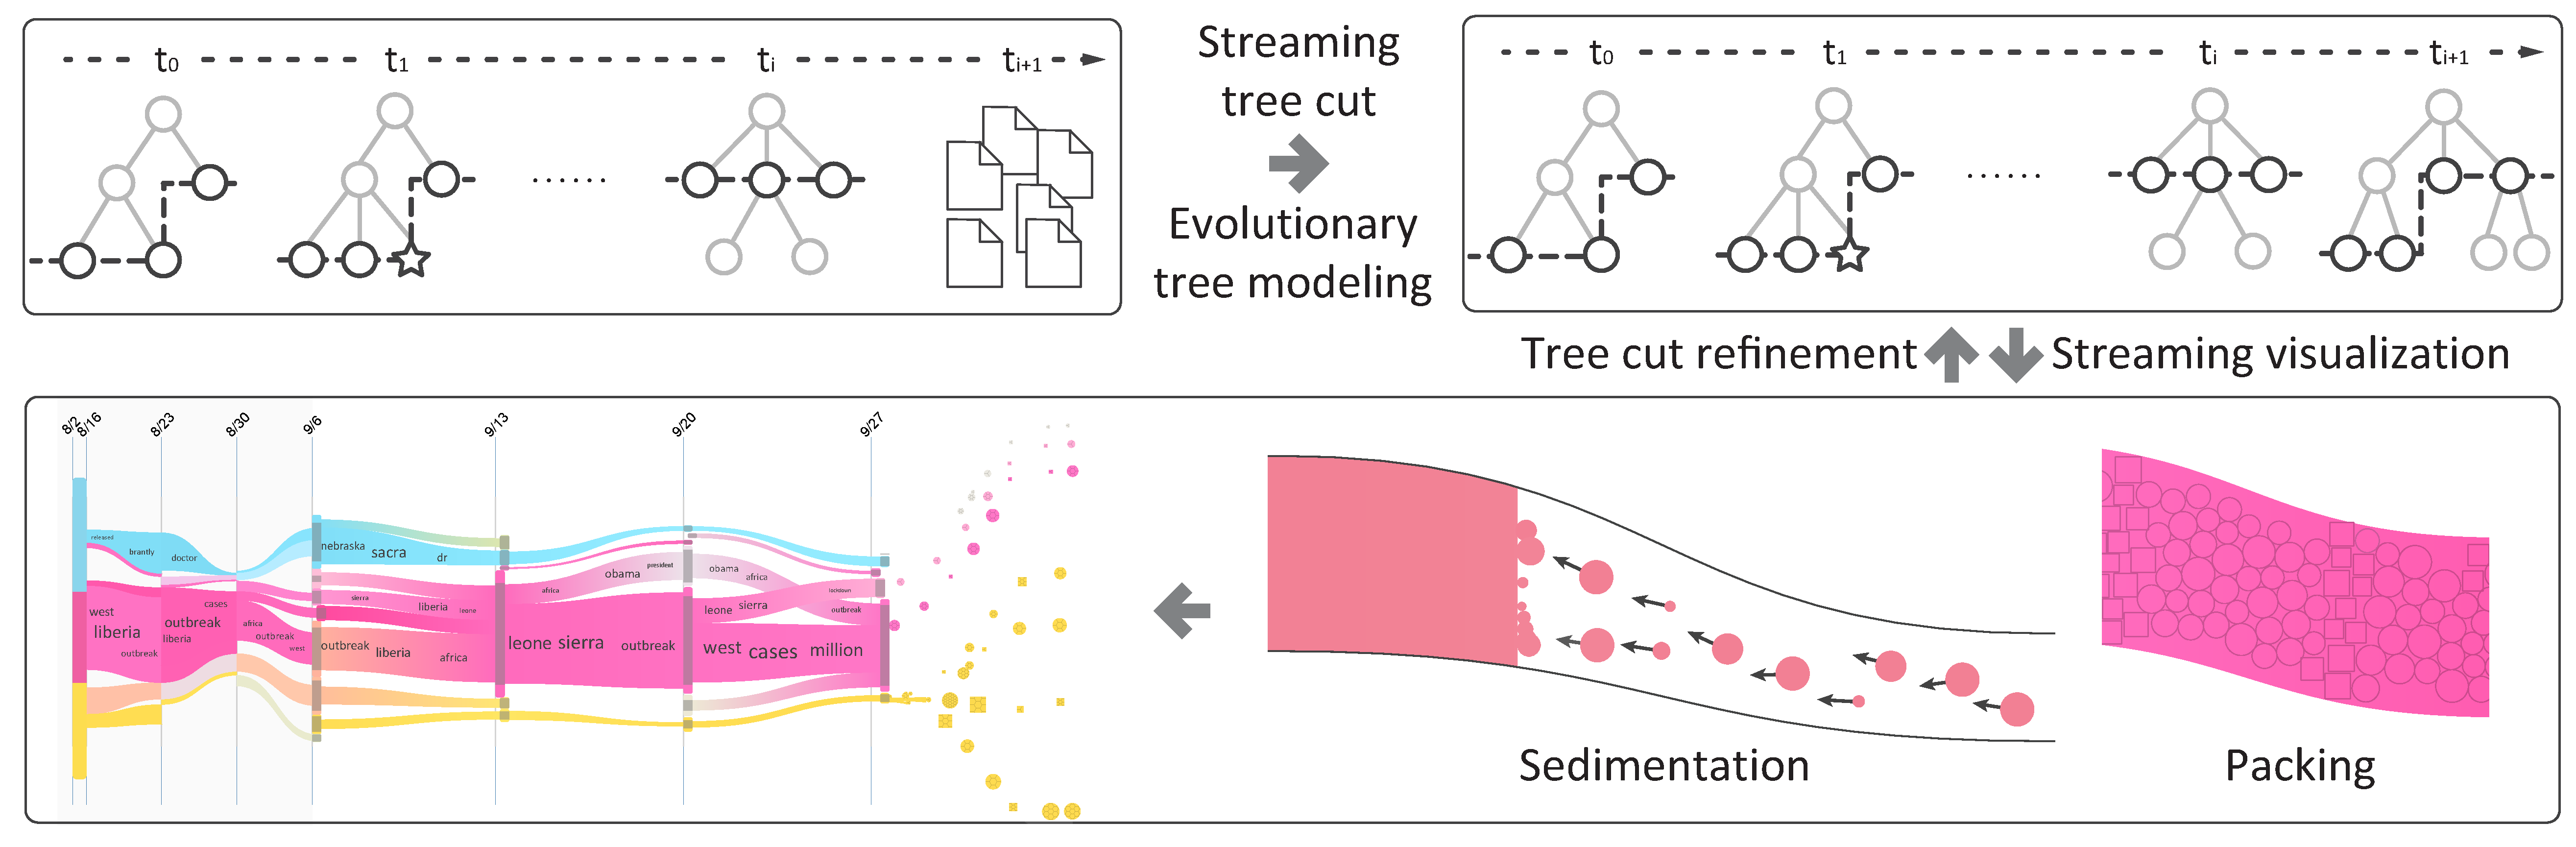
\includegraphics[width=\linewidth]{fig/system}
  \vspace{-5mm}
  \caption{\emph{\normalsize TopicStream} system consists of two modules: streaming tree cut and streaming visualization.}
  \label{fig:overview}
  \vspace{-2mm}
\end{figure*}

\subsection{Evolutionary Topic Analysis}
%Various generative-probabilistic-model-based machine learning algorithms, such as dynamic Latent Dirichlet Allocation (LDA)~\cite{Ahmed2010,blei2006,Blei2012} and hierarchical Dirichlet processes~\cite{Ahmed2008,Xu2008,Xu2008a,Zhang2010}, have been proposed to extract evolving topics from a text stream.
Various generative-probabilistic-model-based machine learning algorithms, such as dynamic Latent Dirichlet Allocation (LDA)~\cite{blei2006} and hierarchical Dirichlet processes~\cite{Ahmed2008,Ahmed2010,Xu2008a,Zhang2010}, have been proposed to extract evolving topics from a text stream.
%To effectively identify a large number of topics from millions of news articles, MemeTracker~\cite{Leskovec2009} was developed.
MemeTracker~\cite{Leskovec2009} was developed to effectively identify phrase-based topics from millions of news articles.
%It provides a coherent representation of the news cycle and  allows users to track the temporal behaviors of memes represented by short phrases.
%\kg{This tool} provides a coherent representation of the news cycle and  allows users to track the temporal \kg{behavior} of memes represented by short phrases.
In many applications, evolving topics may be related to or correspond to one another over time.
%Evolving topics \kg{in many applications can} be related to or correspond \kg{to} one another over time.
The most intuitive relationships are \emph{\normalsize topic correlation}~\cite{wang2007} and \emph{\normalsize common topics}~\cite{wang2009}.
%Recent efforts have also been extended to analyze topic evolution patterns in text data, including topic birth, death, splitting, and merging~\cite{Gao2011}.
Recent efforts have focused on the analysis of topic evolution patterns in text data, including topic birth, death, splitting, and merging~\cite{Gao2011}.
%Although the above-mentioned methods helped users understand a text corpus, none of them focuses on mining and understanding streaming hierarchical topics.
%Although the \kg{aforementioned} methods \kg{help} users understand a text corpus, none of \kg{these} focuses on mining and understanding streaming hierarchical topics.
Although the aforementioned methods help users understand a text corpus, none of them focus on mining and understanding streaming hierarchical topics.

%A previous study has shown that users can better understand and consume information if they are provided with hierarchical topic information over time~\cite{Zhang2009}.
%Some efforts have been exerted recently to mine hierarchical topics and their evolving patterns in temporal datasets efficiently and effectively.
Some efforts have also been exerted recently to mine hierarchical topics and their evolving patterns in temporal datasets.
 %efficiently and effectively.
%The evolutionary hierarchical clustering algorithm~\cite{Chakrabarti2006} aims at generating a sequence of hierarchical clusters.
The evolutionary hierarchical clustering algorithm~\cite{Chakrabarti2006} generates a sequence of hierarchical clusters.
%It aims to cluster data over time.
%The major feature of this algorithm is that clustering at any time fits the current data well.  Furthermore, the clustering does not shift dramatically from one time point to the next when the content is similar.
%The major feature of this algorithm is that clustering \kg{properly} fits current data \kg{at any time}. Furthermore, clustering does not shift dramatically from one time point to the next when \kg{contents} are similar.
The major feature of this algorithm is that clustering properly fits current data at any time (fitness). Furthermore, clustering does not shift dramatically from one time step to the next when content is similar (smoothness).
However, this algorithm can only generate evolving binary trees.
To tackle this issue, Wang et al.~\cite{Wang2013}
% proposed an evolutionary multi-branch tree clustering method.
%In this method, tree construction is formulated as an online posterior estimation problem that considers both the likelihood of the current tree and the conditional prior given the previous tree.
%In this method, tree construction \kg{was} formulated as an online posterior estimation problem that \kg{considered} both the likelihood of the current tree and the conditional prior given the previous tree.
formulated the multi-branch tree construction problem as  a Bayesian online filtering process.
 %that \dc{considers} both the fitness of the current tree and the conditional prior given the previous tree.
%Compared with the method proposed in~\cite{Wang2013}, our method addresses the problem of how to better understand and analyze a sequence of evolutionary multi-branch topic trees.
%\kg{Unlike} the method proposed in~\cite{Wang2013}, our method addresses the problem of \kg{better understanding} and analyze a sequence of evolutionary multi-branch topic trees.
Unlike the method proposed in~\cite{Wang2013}, our method addresses the problem of better understanding and analyzing a sequence of evolutionary multi-branch topic trees.
%Technically, we first learn a set of evolutionary tree cuts from the topic trees based on the user-selected focus nodes.
We first learn a set of evolutionary tree cuts from the topic trees based on the user-selected focus nodes.
%Then we design a time-based interactive visualization to allow users to examine hierarchical topic evolution from multiple perspectives.
Then we design a sedimentation-based interactive visualization to reveal hierarchical topic evolution from multiple perspectives.

%introduce two constraints, triples and fans, into the model to guarantee high smoothness between topic trees. In addition, we also choose the Bayesian rose tree~\cite{Blundell2010} as our base representation to discover multi-branch structures in text data instead of binary tree structures.\looseness=-1

\subsection{Visual Topic and Event Evolution}

The visual analysis of evolving topics in text corpora has been widely studied in recent years~\cite{cui2011,Havre2002,Liu2014survey,Sun2013survey}.
Many methods utilize a river metaphor (a stacked graph) to convey evolving topics over time.
For example, ThemeRiver~\cite{Havre2002} visually depicts how keyword strengths change over time in a text corpus through a river metaphor.
A layer represents a topic in this metaphor.
%The varying width of a layer represents the strength change over time.
The varying width of a layer represents \dc{strength} change over time.
%TIARA~\cite{Liu2009,Liu2012} tightly integrates interactive visualization with topic analysis techniques to help users better understand a document collection.
TIARA~\cite{Liu2009,Liu2012}
%tightly integrates interactive visualization with topic analysis techniques to help users \kg{understand} a document collection.
%In particular, it
%employs the LDA model~\cite{blei2003} to analyze a large text corpus and then
employs an enhanced stacked graph to illustrate how topics evolve over time.
%To model the relationships between evolving topics,
%ParallelTopics~\cite{Dou2011} utilizes ThemeRiver to illustrate topic evolution over time and parallel coordinate plots to reveal the probabilistic distribution of a document on different topics.
ParallelTopics~\cite{Dou2011} utilizes ThemeRiver to illustrate topic evolution over time and parallel coordinate plots to reveal the probabilistic distribution of a document on different topics.
TextFlow~\cite{cui2011} was developed to help analysts visually analyze topic merging and splitting relationships and track their evolution over time.
A visual analysis system was designed by Xu et al.~\cite{Xu2013} to allow analysts to interactively explore and understand the dynamic competition relationships among topics.
% and the influence of opinion leaders.
Recently, Sun et al.~\cite{GSun2014a} extended this work to study both the cooperation and competition relationships among topics.\looseness=-1
%TextFlow~\cite{cui2011} was developed to help analysts visually analyze \kg{the} merging and splitting relationships \kg{of topics} and track their evolution over time.

Several visualization techniques have been proposed recently to help users analyze temporal events and their evolving patterns~\cite{Dou2012,krstajic2013,Luo2012}.
EventRiver~\cite{Luo2012} assumes that clusters of news articles with similar content are adjacent in time and can be mapped to events.
%Thus, this method automatically detects important events and visually presents their impact over time.
Thus, this method automatically detects important events and visually presents their impact over time.
LifeFlow~\cite{Wongsuphasawat2011} and Outflow~\cite{Wongsuphasawat2012} help users explore temporal event sequences.
%\dup{They aggregate multiple event sequences into a tree and a directed acyclic graph, respectively.}
%Timeline visualization is then employed to display the aggregated event sequences from multiple aspects.
%Timeline visualization is then employed to display aggregated event sequences from multiple aspects.\looseness=-1

%In addition, several researchers have proposed word-based approaches to illustrate the content evolution of text data.
%By leveraging the advantages of both parallel coordinates and traditional tag clouds, Collins et al.~\cite{Collins2009} developed Parallel Tag Clouds to support faceted browsing of text corpora.
%Tightly integrating tag clouds with sparklines, SparkClouds~\cite{Lee2010} aimed to visually explain the temporal trend inside tag clouds. To achieve this, it tightly integrated tag clouds with sparklines.

%The above-mentioned approaches focus on the visual exploration of evolving topics/events with flat structures.
%The \kg{aforementioned} approaches focus on visual the visual exploration of evolving topics/events with flat structures.
The aforementioned approaches focus on the visual exploration of evolving topics/events with flat structures.
%Our work attempts to support the visual analysis of evolving hierarchical topics over time.
%\kg{By contrast,} our work attempts to support the visual analysis of evolving hierarchical topics over time.
By contrast, our method attempts to support the visual analysis of evolving hierarchical topics over time.

%HierarchicalTopics~\cite{Dou2013} hierarchically organizes the extracted topics by the BRT model~\cite{Blundell2010,Liu2012} and thus can represent a large number of topics without being cluttered.
HierarchicalTopics~\cite{Dou2013} hierarchically organizes topics using the BRT model~\cite{Blundell2010,Liu2012a}, which can then represent a large number of topics without being cluttered.
%However, this method utilizes one static tree to organize all the topics and cannot illustrate the splitting/merging relationships among topics.
However, this method utilizes one static tree to organize all topics and cannot illustrate splitting/merging relationships among topics.\looseness=-1

To solve this problem, Cui et al.~\cite{cui2014} developed \emph{\normalsize RoseRiver} to progressively explore and analyze the complex evolution patterns of hierarchical topics.
%Cui et al.~\cite{cui2014} made an initial effort to help users progressively explore and analyze the complex evolution patterns of hierarchical topics \kg{and solve the aforementioned problem}.
%This visual analytics system introduces the concept of evolutionary tree cuts and help analysts better understand large document collection with time-stamps.
This system introduces the concept of evolutionary tree cuts to help better understand large document collection with time-stamps.
%However, it fails to provide a mechanism analyze the streaming data because a global evolutionary tree cut algorithm is employed.
However, it fails to provide a mechanism to analyze streaming data because a global tree cut algorithm is employed.
%In addition, the authors used the degree-of-interest-based heuristic rule to derive the key tree cut, which may not be the optimal solution.
In addition, the authors used the DOI-based heuristic rule to derive the key tree cut, which may not be the optimal solution.

%Compared with this method, we employ a posterior probability to derive the optimal tree cut for a selected tree (seed tree cut).
Unlike the preceding method, we employ a-posterior-probability-based method to estimate the fitness of the tree cut.
%In order to help analysts understand the topics of interest in the incoming data, we formulate the derivation of the tree cut in incoming data as the HMM.
We then formulate the derivation of the tree cut in incoming data as a DBN.
% to help analysts understand the topics of interest in incoming data.
%The quantitative evaluation in Sec.~\ref{sec:evaluation} shows that the posterior probability method performs better than the DOI-based method in~\cite{cui2014} for deriving the seed tree cut.
%The quantitative evaluation in Sec.~\ref{sec:evaluation} shows that the posterior probability method performs better than the DOI-based method in~\cite{cui2014} \kg{in} deriving the seed tree cut.
The quantitative evaluation in Sec.~\ref{sec:quantitativeevaluation} shows that the posterior-probability-based method performs better than the DOI-based method in~\cite{cui2014} to fit the focus nodes and topic trees.
%The the performance of the HMM-based streaming evolutionary tree cut algorithm is comparable to that of the global evolutionary tree cut algorithm proposed in~\cite{cui2014}.
The performance of the DBN-based streaming tree cut algorithm is comparable with that of the global tree cut algorithm proposed in~\cite{cui2014}.
%This demonstrates the effectiveness of the proposed mining algorithms in handling the new coming datas in text streams.
%\kg{These observations} demonstrate the effectiveness of the proposed mining algorithms in handling \kg{incoming} data in text streams.
These observations demonstrate the effectiveness of the proposed mining algorithms at handling incoming data in text streams.
%An improved visual sedimentation metaphor~{Huron2013visual} is adopted is visually illustrate how the new coming text streams are aggregating into the existing topic archive.
%An improved visual sedimentation metaphor~\cite{Huron2013visual} is adopted to visually illustrate how \kg{incoming} text streams \kg{aggregate into} existing topics.
An improved visual sedimentation metaphor~\cite{Huron2013visual} has been adopted to visually illustrate how incoming text streams aggregate into existing topics.

%\pei{By saying this, do we mean there are some other methods "to support visual analysis of evolving hierarchical topics over time"?  If so, we have to review those methods.  If not, we need to move the word "among".}

%Inspired by XKCD's movie narrative charts~\cite{RMunroe}, a storyline visualization has been developed to illustrate the temporal interactions between characters in a story.
%Ogawa and Ma~\cite{Ogawa2010} developed a set of heuristic rules to quickly generate a storyline layout.
%Although this method can generate a storyline layout in real time, it may generate a layout with many line crossings and wiggles.
%To overcome this limitation, Tanahashi and Ma~\cite{YTanahashi2012a} formulated the storyline layout as an optimization problem.
%They leveraged spatial information to convey hierarchical relationships among characters.
%However, the hierarchical information was not considered in the layout algorithm but was added in the post-processing step.
%As a result, it cannot leverage the location hierarchy to handle a large number of character lines.
%Different from this method, our method aims to generate a set of evolving topic trees and use them to organize a large number of topics over time.
%To better present evolving hierarchical topics on limited screen real estate, an evolving tree cut algorithm is proposed to extract an appropriate number of topics for each tree, based on the user selected focus node(s).



\section{System Overview}

\emph{\normalsize TopicStream} is designed to track and understand the dynamic characteristics of text streams.
%Accordingly, it consists of two major modules: streaming tree cut and streaming visualization (Fig.~\ref{fig:overview}).
\kg{It} consists of two major modules: streaming tree cut and streaming visualization (Fig.~\ref{fig:overview}).\looseness=-1

%The input of the streaming tree cut is a set of topic trees with tree cuts as well as a set of new coming documents.
The input of the streaming tree cut is a set of topic trees with tree cuts \kg{and} a set of \kg{incoming} documents.
In \emph{\normalsize TopicStream}, the topic trees are derived by the evolutionary tree clustering method developed by Wang et al.~\cite{Wang2013}.
The basic idea of this method is to balance the fitness of a tree and the smoothness between trees by a Bayesian online filtering process.
We derive the tree cuts based on the user-selected focus node(s).
%This module first extracts a topic tree from the newly arrived documents by the evolutionary tree clustering model~\cite{Wang2013}.
This module \kg{initially} extracts a topic tree from the newly arrived documents \kg{using} the evolutionary tree clustering model~\cite{Wang2013}.
%Then a tree cut is derived from the new topic tree via the developed streaming tree cut algorithm.
\kg{A} tree cut is \kg{then} derived from the new topic tree \kg{through} the developed streaming tree cut algorithm.\looseness=-1

%Next, the streaming tree cuts are fed to the visualization module.
The streaming tree cuts are \kg{then} fed into the visualization module.
%We employ the visual sedimentation metaphor to reveal the merging process of newly arrived documents into the dominant center of the visualization, the river part.
We employ the visual sedimentation metaphor to reveal the merging process of newly arrived documents \kg{with} the dominant center of visualization.
% \kg{which is} the river part .
The circle packing algorithm is also developed to illustrate the relationships of document clusters within each topic stripe, including their similarity and temporal relationships~\cite{Wang2006visualization,ZhaoTVCG2014}.\looseness=-1

%% !TEX root = EvoTree-KDD.tex


\section{Evolutionary Tree Clustering}\label{sec:data}
%In this section, we briefly introduce evolutionary multi-branch tree clustering~\cite{Wang2013}, which is used to extract a sequence of multi-branch topic trees \{${T^t}$\} from text streams.
\kg{This section briefly introduces} evolutionary multi-branch tree clustering~\cite{Wang2013}, which is used to extract a sequence of multi-branch topic trees \{${T^t}$\} from text streams.
%To describe the quality of \{${T^t}$\}, two important measures, fitness and smoothness, are employed~\cite{Wang2013}.
Two important measures, \kg{namely,} fitness and smoothness, are employed~\cite{Wang2013} to describe the quality of \{${T^t}$\}.
%The fitness of a tree $T^t$ measures how well the documents at time $t$ are organized.
The fitness of a tree $T^t$ measures how well the documents are organized at time $t$.
%On the other hand, the smoothness ensures the structural similarity between $T^t$ and $T^{t-1}$, if the document content does not deviate much from $t-1$ to $t$.
\kg{Smoothness} ensures the structural similarity between $T^t$ and $T^{t-1}$ if document content does not deviate much from $t-1$ to $t$.
Wang et al.~\cite{Wang2013} formulated the fitness and smoothness in a Bayesian online filtering process \kg{as follows}:
%\dup{To capture both fitness and tree structure changes in the data, we formulated the learning procedure as a Bayesian online filtering process in our previous work~\cite{Wang2013}:}
\begin{equation}\label{eq:learningframework}
\small
\begin{split}
&p(T^t | \mathcal{D}^t, T^{t-1})  \propto  p(\mathcal{D}^t | T^t) p(T^t | T^{t-1}).  \\
%& = \frac{p(\mathcal{D}_m^t|T_m^t)}{p(\mathcal{D}_i^t|T_i^t)p(\mathcal{D}_j^t|T_j^t)} \cdot  \frac{1}{Z} \exp\Big(-\lambda V_{T^{t-1}}(\{T_i^t,T_j^t\} \rightarrow T_m^t)\Big).
\end{split}
\end{equation}
%The first term corresponds to the likelihood ratio of the original BRT algorithm~\cite{Blundell2010} (fitness), and the second term is the smoothness cost.
The first term corresponds to the likelihood ratio of the original BRT algorithm~\cite{Blundell2010} (fitness), whereas the second term \kg{denotes} the smoothness cost.
%This recursive objective function can be solved with a dynamic programming algorithm.
%With this formulation, the new tree $T^t$ depends on the likelihood of the current data $p(\mathcal{D}^t | T^t)$ and the conditional prior $p(T^t | T^{t-1})$ that measures the difference between $T^t$ and $T^{t-1}$.
\kg{Based on} this formulation, the new tree $T^t$ depends on the likelihood of the current data $p(\mathcal{D}^t | T^t)$ and the conditional prior $p(T^t | T^{t-1})$ that measures the difference between $T^t$ and $T^{t-1}$.

%In additional to \textbf{\normalsize a sequence of coherent topic trees \{${T^t}$\}}, the evolutionary tree model also outputs the following two types of information:
In \kg{addition} to \textbf{\normalsize a sequence of coherent topic trees \{${T^t}$\}}, the evolutionary tree model also outputs the following types of information:

\begin{compactitem}
%\item \dup{A sequence of evolving \textbf{topic trees}, where an interior node of a topic tree is a topic and a leaf node is a document.
%In postprocessing, the documents that directly belong to an interior node also form a topic whose parent is the interior node.}
%With this processing, each document is a leaf node.
%\vspace{1mm}
%\item \textbf{\normalsize Topic pairs:} For any adjacent topic trees $T^i$ and $T^{i+1}$, our model maps the related topics together to generate a set of topic pairs. Intuitively, the relations are induced from their document content or the splitting/merging operations taken during the tree generation process.
\item \textbf{\normalsize Topic pairs:} For any adjacent topic trees $T^i$ and $T^{i+1}$, our model maps the related topics \kg{collectively} to generate a set of topic pairs. \kg{The} relations are \kg{intuitively} induced from their document content or \kg{from} splitting/merging operations \kg{performed} during the tree generation process.
%\dup{For two adjacent topic trees, the clustering model maps the related topics, such as similar topics and topics with a splitting/merging relationship, together.}
%\dup{We call two mapped topics a topic pair.}
%\vspace{1mm}
%\item \textbf{\normalsize Document pairs:} For each topic pair between $T^i$ and $T^{i+1}$, our model also maps similar documents together to generate a set of document pairs.
\item \textbf{\normalsize Document pairs:} For each topic pair between $T^i$ and $T^{i+1}$, our model also maps similar documents \kg{collectively} to generate a set of document pairs.
\end{compactitem}


%%\subsection{Clustering Results}
%\dup{Given a text stream, evolutionary tree clustering generates the following outputs.} %\looseness=-1
%
%\begin{compactitem}
%\item \dup{A sequence of evolving \textbf{topic trees}, where an interior node of a topic tree is a topic and a leaf node is a document.
%In postprocessing, the documents that directly belong to an interior node also form a topic whose parent is the interior node.}
%With this processing, each document is a leaf node.
%%\vspace{1mm}
%\item \dup{A set of \textbf{topic pairs} between two adjacent topic trees.}
%\dup{For two adjacent topic trees, the clustering model maps the related topics, such as similar topics and topics with a splitting/merging relationship, together.}
%\dup{We call two mapped topics a topic pair.}
%%\vspace{1mm}
%\item \dup{A group of \textbf{document pairs} within each topic pair. The model also maps two similar documents together, each of which is from each of the topic pairs. These documents are referred to as a document pair.}
%\end{compactitem}

% !TEX root = EvoTree-KDD.tex
% !TEX root = EvoTree-KDD.tex


%\section{Evolutionary Tree Clustering}\label{sec:data}
%%In this section, we briefly introduce evolutionary multi-branch tree clustering~\cite{Wang2013}, which is used to extract a sequence of multi-branch topic trees \{${T^t}$\} from text streams.
%\kg{This section briefly introduces} evolutionary multi-branch tree clustering~\cite{Wang2013}, which is used to extract a sequence of multi-branch topic trees \{${T^t}$\} from text streams.
%%To describe the quality of \{${T^t}$\}, two important measures, fitness and smoothness, are employed~\cite{Wang2013}.
%Two important measures, fitness and smoothness, are employed~\cite{Wang2013} to describe the quality of \{${T^t}$\}.
%%The fitness of a tree $T^t$ measures how well the documents at time $t$ are organized.
%The fitness of a tree $T^t$ measures how well the documents are organized at time $t$.
%%On the other hand, the smoothness ensures the structural similarity between $T^t$ and $T^{t-1}$, if the document content does not deviate much from $t-1$ to $t$.
%\kg{Smoothness} ensures the structural similarity between $T^t$ and $T^{t-1}$ if document content does not deviate much from $t-1$ to $t$.
%Wang et al.~\cite{Wang2013} formulated the fitness and smoothness in a Bayesian online filtering process \kg{as follows}:
%%\dup{To capture both fitness and tree structure changes in the data, we formulated the learning procedure as a Bayesian online filtering process in our previous work~\cite{Wang2013}:}
%\begin{equation}\label{eq:learningframework}
%\small
%\begin{split}
%&p(T^t | \mathcal{D}^t, T^{t-1})  \propto  p(\mathcal{D}^t | T^t) p(T^t | T^{t-1}).  \\
%%& = \frac{p(\mathcal{D}_m^t|T_m^t)}{p(\mathcal{D}_i^t|T_i^t)p(\mathcal{D}_j^t|T_j^t)} \cdot  \frac{1}{Z} \exp\Big(-\lambda V_{T^{t-1}}(\{T_i^t,T_j^t\} \rightarrow T_m^t)\Big).
%\end{split}
%\end{equation}
%%The first term corresponds to the likelihood ratio of the original BRT algorithm~\cite{Blundell2010} (fitness), and the second term is the smoothness cost.
%The first term corresponds to the likelihood ratio of the original BRT algorithm~\cite{Blundell2010} (fitness), whereas the second term \kg{denotes} the smoothness cost.
%%This recursive objective function can be solved with a dynamic programming algorithm.
%%With this formulation, the new tree $T^t$ depends on the likelihood of the current data $p(\mathcal{D}^t | T^t)$ and the conditional prior $p(T^t | T^{t-1})$ that measures the difference between $T^t$ and $T^{t-1}$.
%\kg{Based on} this formulation, the new tree $T^t$ depends on the likelihood of the current data $p(\mathcal{D}^t | T^t)$ and the conditional prior $p(T^t | T^{t-1})$ that measures the difference between $T^t$ and $T^{t-1}$.

%In additional to \textbf{\normalsize a sequence of coherent topic trees \{${T^t}$\}}, the evolutionary tree model also outputs the following two types of information:
%In \kg{addition} to \textbf{\normalsize a sequence of coherent topic trees \{${T^t}$\}}, the evolutionary tree model also outputs the following types of information:
%
%\begin{compactitem}
%%\item \dup{A sequence of evolving \textbf{topic trees}, where an interior node of a topic tree is a topic and a leaf node is a document.
%%In postprocessing, the documents that directly belong to an interior node also form a topic whose parent is the interior node.}
%%With this processing, each document is a leaf node.
%%\vspace{1mm}
%%\item \textbf{\normalsize Topic pairs:} For any adjacent topic trees $T^i$ and $T^{i+1}$, our model maps the related topics together to generate a set of topic pairs. Intuitively, the relations are induced from their document content or the splitting/merging operations taken during the tree generation process.
%\item \textbf{\normalsize Topic pairs:} For any adjacent topic trees $T^i$ and $T^{i+1}$, our model maps the related topics \kg{collectively} to generate a set of topic pairs. \kg{The} relations are \kg{intuitively} induced from their document content or \kg{from} splitting/merging operations \kg{performed} during the tree generation process.
%%\dup{For two adjacent topic trees, the clustering model maps the related topics, such as similar topics and topics with a splitting/merging relationship, together.}
%%\dup{We call two mapped topics a topic pair.}
%%\vspace{1mm}
%%\item \textbf{\normalsize Document pairs:} For each topic pair between $T^i$ and $T^{i+1}$, our model also maps similar documents together to generate a set of document pairs.
%\item \textbf{\normalsize Document pairs:} For each topic pair between $T^i$ and $T^{i+1}$, our model also maps similar documents \kg{collectively} to generate a set of document pairs.
%\end{compactitem}




\section{Streaming Tree Cut}\label{sec:tree-cut}
%In this section, we introduce how to derive the new tree cut incrementally as new text data arrives.
\kg{This section explains} how \kg{a} new tree cut \kg{is} incrementally \kg{derived} as new text data arrives.

%In particular, the algorithm contains two parts: construction of evolving tree cuts and reorganization of the topics on each tree cut.

\subsection{Problem Formulation}

%As in~\cite{cui2014}, we use the tree cut to represent a topic tree based on the user's interest.
%\kg{We} use the tree cut to represent a topic tree based on the \kg{interest of the user, which is similar to~\cite{cui2014}}.
\kg{We} use \docpr{a} tree cut to represent a topic tree based on user interests, which is similar to~\cite{cui2014}.
%A \textbf{\normalsize tree cut} is a set of nodes wherein every path from the root of the tree to a leaf contains exactly one node from the cut.
%A \textbf{\normalsize tree cut} is a set of nodes \kg{where} every path from the root of the tree to a leaf contains exactly one node from the cut.
A \textbf{\normalsize tree cut} is a set of nodes \dc{in which} every path from the root of the tree to a leaf contains exactly one node from the cut.
%Naturally, each cut could be regarded as a clustering result for the documents at that time point.
Thus, each cut can be used as a set of representative topic nodes.
%In other words, a tree cut represents a level of topic granularity of a user's interest.
%\kg{That is}, a tree cut represents a level of topic granularity of a user's interest.
\kg{That is}, a tree cut represents a level of topic granularity of a user's \docpr{interests}.
Fig.~\ref{fig:treecutexample} represents an example of a tree cut.
%To facilitate the following discussion,
We refer to each node on the tree cut as a ``\textbf{\normalsize cut node}.''

%\pei{One may ask whether specifying a complete initial tree cut can be tedious and difficult for a user, since it requires EVERY path from the root to a leaf has a cut node.  If a tree has thousands of leaf nodes, a tree cut may contain hundreds of nodes.  Can we say something to comfort such a concern?  Section 4.1.2 seems to address this issue.  If so, we should assure readers and pu a pointer here to Section 4.1.2.}

%In the first step of data transformation, we design an algorithm to produce meaningful tree cut for each topic tree given a user focus topic.

\begin{figure}[t]
  \centering
  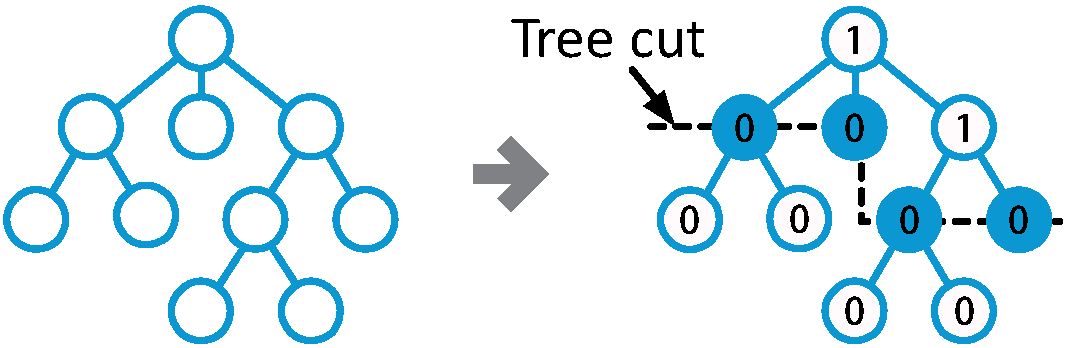
\includegraphics[width=2.5in]{fig/treecut}
  %\vspace{-mm}
  \caption{
%  \small
%  Tree cut example: the cut is denoted by the dotted line. Every node above the dotted line is labeled 1, while the rest are labeled 0.
Tree cut example: the cut is denoted by the dotted line. Every node above the dotted line is labeled 1, while the \docpr{others} are labeled 0.
}
  \label{fig:treecutexample}
  \vspace{-5mm}
\end{figure}



%The basic principle behind determining a set of optimal tree cuts is that each tree cut in the sequence should be similar to the one at the previous time point if the tree structures are similar (smoothness).
The basic principle \kg{to determine} a set of optimal tree cuts is that each tree cut in the sequence should be similar to the one at the previous time step if the tree structures are similar (smoothness).
%The tree cut must also adequately represent user interest and the topic tree at that time point (fitness).
The tree cut must also adequately represent user interests and the topic tree at that time step (fitness).
%Here the optimal tree cut is the cut that leads to the best similarity to the focus node(s) and the best representation for the tree (fitness).
%One straightforward method is to manually label all the tree cuts.
%Unfortunately, this method requires the user to examine every path from the root to a leaf to select a proper cut node.
%As a result, it \shixia{requires knowledge and skills and is very time-consuming,} especially when there are hundreds of topic trees and each of which contains hundreds of or even thousands of nodes.
%The global evolutionary tree cut algorithm developed in~\cite{cui2014} computes all the tree cuts together, based on the seed tree cut.
The global tree cut algorithm developed in~\cite{cui2014} computes all tree cuts \kg{simultaneously} based on the focused nodes.
%There are two problems when applying it to the text stream.
\kg{Two} problems arise when applying \kg{the aforementioned algorithm} to the text stream.
%First, it is very time consuming if we compute all the tree cut again when the new text data arrives.
First, it is very time consuming \docpr{to} compute all the tree \docpr{cuts each time} new text data arrives.
%First, \kg{computing} all the tree \kg{cuts once more} when new text data arrive \kg{is time-consuming}.
%Second, if the tree cuts are computed again with the new data, the existing tree cuts will be changed to some extent, which is difficult for analyst to maintain their visual momentum~\cite{Woods1984}.
%Second, if the tree cuts are computed again with new data, \kg{then} the existing tree cuts \kg{are} changed to \kg{a certain} extent, which \kg{makes maintaining the} visual momentum \kg{of analysts difficult}~\cite{Woods1984}.
%Second, if the tree cuts are computed again with \dc{the} new data, \kg{then} the existing tree cuts \kg{are} changed to \kg{a certain} extent, which \kg{makes maintaining the} visual momentum \dc{of analysts difficult}~\cite{Woods1984}.
Second, if the tree cuts are \docpr{recomputed along} with \dc{the} new data, \kg{then} the existing tree cuts \kg{are} changed to \kg{a certain} extent, which \kg{makes maintaining the} mental map \dc{of analysts difficult}~\cite{Woods1984}.


\begin{figure}[t]
  \centering
  % Requires \usepackage{graphicx}
  \includegraphics[width=2.1in]{fig/hmm2}
  \caption{
  %The dynamic Bayesian network for deriving streaming tree cuts.
  Dynamic Bayesian network for deriving streaming tree cuts. Here $T^t$ and ${\phi}^t$ are the topic tree and tree cut at \emph{t}.
  }\label{fig:hmm}
  \vspace {-5mm}
\end{figure}


\begin{table}[b]
\small
    \vspace{-5mm}

    \centering
    \scalebox{0.8}{

    \begin{tabular}{|c|c|}
    \hline
    %Data & Time span & N\_num & T\_num & Depth & I\_num \\
    \textbf{Notation} & \textbf{Definition} \\
   % Notation & Definition \\
    \hline
   %\multicolumn{2}{|c|}{Symbols} \\
   %\hline
   	$T^t$ & The topic tree at time $t$ \\
   \hline
	$\phi^t$ & The tree cut at time $t$ \\
	\hline
	$m$ & Number of focus nodes selected by the user \\
	\hline
	$T_{fi}$ &  The $i$th focus node \\
	\hline
	$\mathcal{D}_{fi}$ &  The document set of the $i$th focus node\\
	\hline	
	$ p({\phi}^t|{\phi}^{t-1},T^t)$ & The conditional distribution of $\phi^t$ according to DBN \\
	\hline
	$p({\phi}^t|T^t)$ & \tvcgminor{Fitness of tree cut ${\phi}^t$ to $T^t$} \\
	\hline
	$p({\phi}^t|{\phi}^{t-1})$ & Smoothness between adjacent tree cuts $\phi^t$ and $\phi^{t-1}$ \\
   \hline	
   	\tvcgminor{$p({\phi}^t|\mathcal{D}_{f0}, ..., \mathcal{D}_{fm})$} & The posterior probability of a tree cut ${\phi}^t$ \\
	\hline   	
	$E_1(T^t)$ & The similarity energy of the topic tree $T^t$ \\
   	\hline	
	$T_r$, $T_s$ &  A topic node (an internal node) in the topic tree \\
	\hline	   	
   	$\mathbf{S}(T_r,T_s)$ & The cosine similarity between topic nodes $T_r$ and $T_s$ \\
   	\hline	
	$l_s$ &  The label (0 or 1, see Fig.~\ref{fig:treecutexample}) of topic node $T_s$  \\
	\hline	
   	$E_2(\phi^{t}, \phi^{t-1})$ & The smoothness energy between tree cuts $\phi^t$ and $\phi^{t-1}$ \\
   	\hline	   	
	$\mathcal{D}_s$ &  The document set of topic node $T_s$\\
	\hline	
    $f_{DCM}(\mathcal{D})$  & The marginal distribution of document set $\mathcal{D}$ \\	
	\hline
	$\mathbf{WS}(T_c)$ &  Window size for $T_c$ in mean-shift clustering \\
	\hline
   %\multicolumn{2}{|c|}{Functions} \\
   %\hline
    \end{tabular}
    }
       \caption{
    \tvcgminor{Frequently used notations in the model.} %Sec.~\ref{sec:tree-cut}.}
    }
     \label{table:notations}
%   \vspace{-5mm}
\end{table}

%To solve these problems, we adopt a dynamic Bayesian network (DBN) to infer the tree cut for the incoming text data that is organized by a topic tree.
%To solve \kg{the aforementioned} problems, we adopt a dynamic Bayesian network (DBN) model to infer the tree cut for the incoming text data organized by a topic tree.
To solve \kg{the aforementioned} problems, we \docpr{have adopted} a dynamic Bayesian network (DBN) model to infer the tree cut for the incoming text data organized by a topic tree.
%Previous studies have shown that adopting overlapping successive views to support continuity across data sets is a frequently adopted principle for processing temporal data~\cite{Chakrabarti2006,Woods1984}.
Previous studies have shown that adopting overlapping successive views to support continuity across data sets is a frequently adopted principle \kg{to process} temporal data~\cite{Chakrabarti2006,Woods1984}.
%In our case, the new tree cut ${\phi}^t$ is relevant to the tree cuts adjacent to it in time as well as $T^t$ (Fig.~\ref{fig:hmm}).
In our case, the new tree cut ${\phi}^t$ is relevant to temporally \kg{adjacent} tree cuts as well as $T^t$ (Fig.~\ref{fig:hmm}).
%Specifically, topic mapping between adjacent trees is utilized as a constraint to smoothen the tree cut transitions over time.
\kg{In particular}, topic mapping between adjacent trees is utilized as a constraint to \dc{smooth} tree cut transitions over time.
%Based on this principle, we adopt  \looseness=-1
%The algorithm involves three steps: 1) users specify one or more topic nodes as the focus node(s); 2) the seed tree cut(s) is generated based on the user selected focus topic(s) and a posterior probability distribution; 3) a set of evolving tree cuts are derived based on the seed tree cut(s).

%For the sake of simplicity, we take one focus node as an example to illustrate the evolving tree cut algorithm.

\subsection{Model}

%In this section, we study the problem of identifying a set of coherent tree cuts in the topic trees given a small number of user-selected focus nodes.

%After deriving the seed tree cuts, we then propagate them to other topic trees, including the new coming topic trees, to generate a set of coherent tree cuts.
%The problem of tree cut propagation can be formulated as a labeling problem, in which the topic nodes above the tree cut are labeled 1 and the rest (including the cut nodes) are labeled 0 (Fig.~\ref{fig:treecutexample}).


\begin{figure*}[t]
\centering
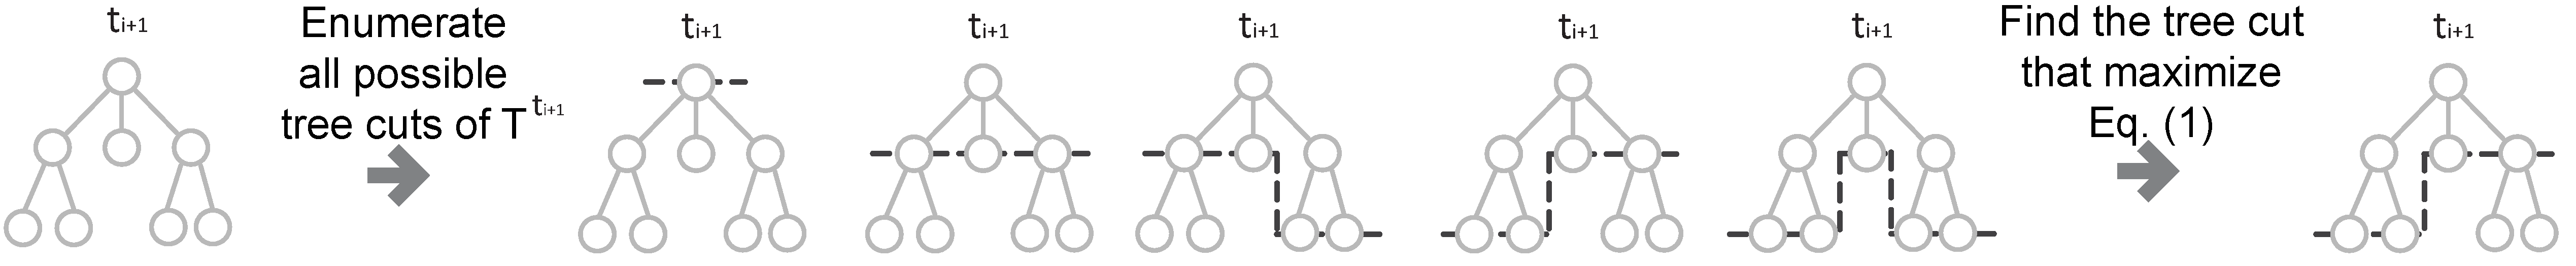
\includegraphics[width=0.9\textwidth]{fig/treecutalgorithm2}
\caption{\tvcgminor{Streaming tree cut algorithm: given the incoming topic tree $T^{t_{i+1}}$, we enumerate all possible tree cuts of $T^{t_{i+1}}$ and then pick the tree cut that maximizes Eq.~(\ref{eq:hmm1}).}}
\vspace{-5mm}
\label{fig:treecutalgorithm}
\end{figure*}


%Assume we already have a sequence of topic trees and the corresponding tree cuts based on users' interest, the problem of deriving the new tree cut in a text stream can be regarded as a labeling problem.
Assume \kg{that} we already have a sequence of topic trees and the corresponding tree cuts.
\kg{The} problem of deriving \kg{a} new tree cut in a text stream can \kg{then} be regarded as a labeling problem.
%In the labeling, the topic nodes above the tree cut are labeled 1 and the rest (including the cut nodes) are labeled 0 (Fig.~\ref{fig:treecutexample}).
\kg{The} topic nodes above the tree cut are labeled 1\kg{, whereas} the rest (including the cut nodes) are labeled 0 (Fig.~\ref{fig:treecutexample}).
We first introduce some frequently used notations in Table~\ref{table:notations}, which are useful for subsequent discussions.
%\tvcgminor{Table~\ref{table:notations} summarizes the notations commonly used in this section.}

%as an HMM.
%Given $m$ focus nodes \{${T_{fi}}$\} with document sets \{$\mathcal{D}_{fi}$\}, we aim to infer the tree cut ${\phi}^t$ in the new coming topic tree $T^t$.
%Given $m$ focus nodes \{${T_{fi}}$\} with document sets \{$\mathcal{D}_{fi}$\}, we infer the tree cut ${\phi}^t$ in the new coming topic tree $T^t$.
Given \emph{\normalsize m} focus nodes \{${T_{fi}}$\} with document sets \{$\mathcal{D}_{fi}$\}, we infer the tree cut ${\phi}^t$ in the \dc{incoming} topic tree $T^t$.
%In deriving the optimal tree cut, we consider both fitness (likelihood) and the expected node number that can be accommodated by the display area.
%As shown in Fig.~\ref{fig:hmm}, $T^t$ is an observation and ${\phi}^t$ is a hidden variable.
Fig.~\ref{fig:hmm} \kg{shows that} $T^t$ is an observation \kg{variable} and ${\phi}^t$ is a hidden variable.
%The relationship between ${\phi}^t$ and ${\phi}^{t-1}$ as well as $T^t$ can be modeled by DBN.
The relationship between ${\phi}^t$ and \docpr{${\phi}^{t-1}$, as well as $T^t$, can} be modeled by DBN.
Accordingly, the conditional distribution of ${\phi}^t$ is $p({\phi}^t|{\phi}^{t-1},T^t)$.
%On the other hand, ${\phi}^t$ is relevant to $\mathcal{D}_{f0},\mathcal{D}_{f1}, ..., \mathcal{D}_{fm}$ at each time $t$, we then formulate the inference of the new tree cut as
Since ${\phi}^t$ is relevant to $\mathcal{D}_{f0},\mathcal{D}_{f1}, ..., \mathcal{D}_{fm}$ at each time $t$, we formulate the inference of the new tree cut as:

\vspace{-5mm}
\begin{equation}
max\ p({\phi}^t,{\phi}^{t-1}, ...,{\phi}^0|\mathcal{D}_{f0},\mathcal{D}_{f1}, ..., \mathcal{D}_{fm})\cdot p({\phi}^t|{\phi}^{t-1},T^t).
\label{eq:hmm1}
\end{equation}


%\begin{figure*}
%\centering
%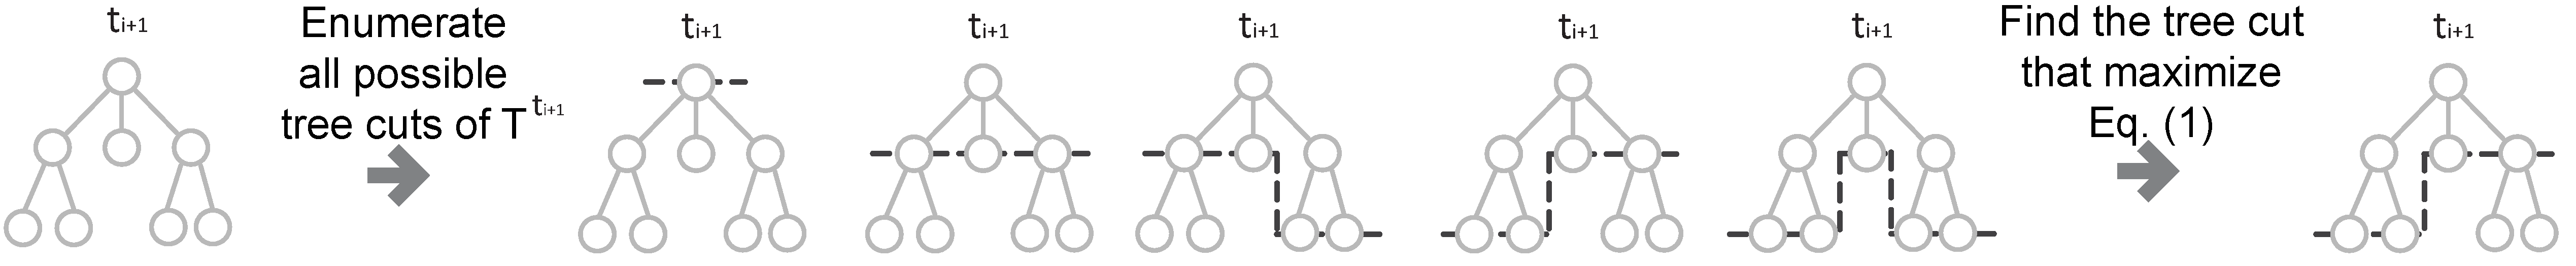
\includegraphics[width=0.9\textwidth]{fig/treecutalgorithm2}
%\caption{\tvcgminor{Streaming tree cut algorithm: given the incoming topic tree $T^{t_{i+1}}$, we enumerate all possible tree cuts of $T^{t_{i+1}}$ and then select the tree cut that maximizes Eq.~(\ref{eq:hmm1}).}}
%\vspace{-5mm}
%\end{figure*}

\tvcgminor{As shown in Fig.~\ref{fig:treecutalgorithm}, the goal is to find the tree cut that maximizes Eq.~(\ref{eq:hmm1}).
%Next, we describe how to calculate Eq.~(\ref{eq:hmm1}).
}

%Given $\mathcal{D}_{f0},\mathcal{D}_{f1}, ..., \mathcal{D}_{fm}$, ${\phi}^t, {\phi}^{t-1}, ..., {\phi}^0$ are conditionally independent, Eq.~\ref{eq:hmm1} can be rewritten as
%Given $\mathcal{D}_{f0},\mathcal{D}_{f1}, ..., \mathcal{D}_{fm}$, ${\phi}^t, {\phi}^{t-1}, ..., {\phi}^0$ are conditionally independent, Eq.~\ref{eq:hmm1} can be rewritten as
Since ${\phi}^t, {\phi}^{t-1}, ..., {\phi}^0$ are conditionally independent given $\mathcal{D}_{f0},\mathcal{D}_{f1}, ..., \mathcal{D}_{fm}$,
the first term is computed by $\prod\limits_{\tau=0}^{t}p({\phi}^\tau|\mathcal{D}_{f0},\mathcal{D}_{f1}, ..., \mathcal{D}_{fm})$.
According to the graphical model of DBN (Fig.~\ref{fig:hmm}), the second term is proportional to $p({\phi}^{t}|T^{t})p({\phi}^{t}|{\phi}^{t-1})$.
\xiting{Because} ${\phi}^{t-1},\ {\phi}^{t-2},...,\ {\phi}^{0}$ are known, Eq.~(\ref{eq:hmm1}) can be simplified as:
%\begin{equation}
%\small
%max\ \prod_{\tau=0}^{t}p({\phi}^{\tau}|\mathcal{D}_{f0},\mathcal{D}_{f1}, ..., \mathcal{D}_{fm})p({\phi}^{\tau}|T^{\tau})\prod_{\tau=1}^{t}p({\phi}^{\tau}|{\phi}^{\tau-1}).
%\label{eq:hmm1.5}
%\end{equation}
%%Here $p({\phi}^t|T^t)$ denotes how well the tree cut ${\phi}^t$ represents $T^t$, which is measured by the similarity energy $\mathbf{E}_1$:

\vspace{-4mm}
\begin{equation}
%\small
max\ p({\phi}^t|T^t)p({\phi}^{t}|{\phi}^{t-1})p({\phi}^{t}|\mathcal{D}_{f0},\mathcal{D}_{f1}, ..., \mathcal{D}_{fm}).
\label{eq:hmm2}
\end{equation}

$p({\phi}^t|T^t)$ denotes how well the tree cut ${\phi}^t$ represents $T^t$, which is measured by the similarity energy $\mathbf{E}_1$ in the form of $p({\phi}^t|T^t) = e^{-E_1(T^t)}$.
%$\mathbf{E}_1$ measures the content similarity of each topic $T_r$ in $T^t$ to the two topic sets, which are topic nodes sets labeled 0 and 1 respectively.
$\mathbf{E}_1$ measures the content similarity of each topic $T_r$ in $T^t$ \docpr{for} the two topic sets, which are topic \docpr{node} sets labeled 0 and \docpr{1, respectively}.
%It can be derived as follows:

\vspace{-3mm}
\begin{equation}
\small
E_1(T^t) = \sum_{T_r\in{\mathcal{N}^t}}\min_{T_s\in{\mathcal{N}^t},l_s=l_r}(-\log(\mathbf{S}(T_r,T_s))),
\end{equation}
where $l_r$ is the label (1 or 0) of topic node $T_r$, $\mathcal{N}^t$ is the set which contains all tree nodes in $T^t$.
%Similarity energy $\mathbf{E}_1$ measures the content similarity of topic $T_r$ to the two topic sets, \{1\} and \{0\}.
%\{1\} and \{0\} represent the nodes with fixed labels as 1 and 0.
%\{1\} and \{0\} represent \dc{nodes} with \dc{the} fixed labels \dc{1} and 0.
%At this step, they only contain the topic nodes in the key topic tree, as they are the only nodes with fixed labels.
%It measures the cost of node $r$ to the key label model built from the key tree cut.
%For a topic $T_r$, cosine similarity $\mathbf{S}(T_r,T_s)$ is used to compute the similarity value between $T_r$ and each topic $T_s$ in \{1\} or \{0\}.
For a topic $T_r$, \kg{the} cosine similarity $\mathbf{S}(T_r,T_s)$ is used to compute the similarity value between $T_r$ and $T_s$ with the same label.

$p({\phi}^t|{\phi}^{t-1})$ measures the smoothness cost between two adjacent tree cuts using the smoothness energy $\mathbf{E_2}$, which is defined as $p({\phi}^t|{\phi}^{t-1})= e^{-E_2(\phi^t,\phi^{t-1})}$. $\mathbf{E_2}$ measures the mapping similarity between $T^t$ and $T^{t-1}$:
\vspace{-3mm}
\begin{equation}
E_2(\phi^t,\phi^{t-1}) = \sum\limits_{T_r\in{\mathcal{N}^t},T_s\in{\mathcal{N}^{t-1}}}|l_r-l_s|\varphi(l_r,l_s),
\label{eq:hmm5}
\end{equation}
where $\varphi(l_r,l_s)$ denotes the mapping weight computed by the evolutionary tree clustering model.


%we calculate its similarity values to all the nodes in the key topic tree and treat the minimum one as its similarity value to the .
%Particularly, $\mathbf{E}_1(x_r)$ is defined as:
%\kg{In particular}, $\mathbf{E}_1(x_r)$ is defined as:
%
%\small
%\[
%\mathbf{E}_1(x_r)=
%    \begin{cases}
%    	0,     &\text{if  $T_r\in\{x_r\}$;}\\
%        \infty,&\text{if  $T_r\in\{1-x_r\}$;}\\
%        \min_{T_r\in\{x_r\}}(-\log(\mathbf{S}(T_r,T_s))), & \text{otherwise.}\\
%    \end{cases}
%\]
%\normalsize
%, $\mathcal{T}$ represents all the topics in the tree sequence,

%$p({\phi}^t|{\phi}^{t-1})$ measures the smoothness cost between two adjacent tree cuts.
%$p({\phi}^t|\mathcal{D}_{f0},\mathcal{D}_{f1}, ..., \mathcal{D}_{fm})$ is defined as a posterior probability of a tree cut ${\phi}^t$
$p({\phi}^t|\mathcal{D}_{f0},\mathcal{D}_{f1}, ..., \mathcal{D}_{fm})$ is defined as a posterior probability of a tree cut ${\phi}^t$\kg{. Thus,}
%and $p({\phi}^t)$ indicates the prior preference of the node number for the tree cut, which are defined as below.

%\subsubsection{Seed Tree Cut}
%we utilize a posterior probability to derive the optimal tree cut for a tree.
%Thus, we formulate the posterior probability of a tree cut $\phi$ as
\vspace{-5mm}
\begin{equation}
\label{eq:seed}
p({\phi}^t|\mathcal{D}_{f0}, \mathcal{D}_{f1}, ..., \mathcal{D}_{fm}) \propto p(\mathcal{D}_{f1}, \mathcal{D}_{f2}, ..., \mathcal{D}_{fm}|{\phi}^t) p({\phi}^t),
\end{equation}
where $p(\mathcal{D}_{f0}, \mathcal{D}_{f1}, ..., \mathcal{D}_{fm}|{\phi}^t)$ is the likelihood of the tree cut.
$p({\phi}^t)$ indicates the prior preference of the node number for the tree cut.
The tree cut that results in maximum posterior probability is the optimal tree cut.
%In our model, we derive the optimal tree cut(s) in the tree(s) that the focus node(s) belong to and regard them as the seed tree cut(s).
%We select such a tree cut because it can adequately represent the information needs of the user.

$p({\phi})$ is defined as $e^{-\lambda|\mathcal{C}_{{\phi}}|}$, where $\mathcal{C}_{{\phi}}$ is the set of topics in ${\phi}$, $|\mathcal{C}_{\phi}|$ is the node number in the tree cut, and $\lambda$ is the parameter that balances the
likelihood and expected node number.\looseness=-1

%We then illustrate how to calculate the likelihood of a tree cut.  for shixia
We then illustrate how the likelihood of a tree cut \kg{can be calculated}.
%We adopt a prediction model to estimate the likelihood of every possible tree cut.
We adopt a prediction model to estimate the likelihood of \kg{each} possible tree cut.
%For simplicity, we begin with one focus node. %with document set $\mathcal{D}_f$.
For simplicity\dc{'s sake}, we begin with one focus node. %with document set $\mathcal{D}_f$.
%\kg{We} begin with one focus node \kg{for simplicity}. %with document set $\mathcal{D}_f$.
%Given a focus node $T_f$ and its corresponding document set $\mathcal{D}_f$, the predictive probability of a tree cut $\phi$ is defined as
Given a focus node $T_f$ and its corresponding document set $\mathcal{D}_f$, the predictive probability of a tree cut $\phi$ is defined as: %\kg{follows:}
\begin{equation}
%\small
p(\mathcal{D}_f|\phi) = \sum_{T_s\in \mathcal{C}_{\phi}} \omega_s p(\mathcal{D}_f|\mathcal{D}_s),
\end{equation}
where $\mathcal{C}_{\phi}$ is the set of topics in $\phi$ and $\omega_s$ is the prior probability that all the documents in $\mathcal{D}_f$ belong to $\mathcal{D}_s$.
To calculate $\omega_s$, we assume that the probability of a set of documents belonging to a specific topic is proportional to the number of documents in that topic~\cite{Blundell2011}.
%\kg{We assume} that the probability of a set of documents \kg{belonging to} a specific topic is proportional to the number of documents in that topic \kg{to calculate $\omega_S$}~\cite{Blundell2011}.
Accordingly, we obtain $\omega_s = {|\mathcal{D}_s|}/{|\mathcal{D}_a|}$.
%$\mathcal{D}_a$ includes all documents in the tree.
$\mathcal{D}_a$ includes all documents in \kg{a} tree.
%$p(\mathcal{D}_f|\mathcal{D}_S)$ is the predictive distribution of the corresponding topic model
$p(\mathcal{D}_f|\mathcal{D}_s)$ is the predictive distribution of the corresponding \xiting{topic model.}
\begin{equation}
\small
p(\mathcal{D}_f|\mathcal{D}_s) = {f(\mathcal{D}_f \cup \mathcal{D}_s)}/{f(\mathcal{D}_s)},
\end{equation}
where $f(\mathcal{D})$ is the marginal probability of data $\mathcal{D}$.

%Dirichlet compound multinomial (DCM) distribution is derived based on multinomial and Dirichlet conjugate distributions~\cite{Liu2012, RasmusMadsen2005}.
\kg{The} Dirichlet compound multinomial (DCM) distribution is derived \kg{from} multinomial and Dirichlet conjugate distributions~\cite{Liu2012a}.
%Considering that DCM relies on hierarchical Bayesian modeling techniques, it is a more appropriate generative model than the traditional multinomial distribution for text documents.
%Considering that \kg{it} relies on hierarchical Bayesian modeling techniques, \kg{DCM} is a more appropriate generative model than the traditional multinomial distribution for text documents.
\dc{Because} \kg{it} relies on hierarchical Bayesian modeling techniques, \kg{DCM} is a more appropriate generative model than the traditional multinomial distribution for text documents.
%Thus, we utilize the DCM distribution to represent the marginal distribution $f(\mathcal{D})$ .
Thus, we utilize the DCM distribution to represent the marginal distribution $f(\mathcal{D})$ \kg{as follows:}
\begin{equation}
\label{eq:dcm}
%\small
f_{DCM}(\mathcal{D}) =  \prod_i^n \frac{(\sum_j^{|\mathcal{V}|}z_i^{(j)})!}{\prod_j^{|\mathcal{V}|} z_i^{(j)}!} \cdot \frac{\Delta({\bm \alpha}+\sum_i\bold{z}_i)}{\Delta({\bm \alpha})},
\end{equation}
where \xiting{$|\mathcal{V}|$ is the vocabulary size, $\bold{z}_i\in \mathcal{R}^{|\mathcal{V}|}$ is the word vector of the $i$th document, and $z_i^{(j)}$ is the frequency of the $j$th term.} % in the $i$th document
%${\bm \alpha} = (\alpha^{(1)},\alpha^{(2)},\ldots,\alpha^{(|\mathcal{V}|)})^T \in \mathcal{R}^{|\mathcal{V}|}$ is the parameter that controls the Dirichlet distribution, which is the prior of the multinomial distribution of each topic.
${\bm \alpha} = (\alpha^{(1)},\alpha^{(2)},\ldots,\alpha^{(|\mathcal{V}|)})^T \in \mathcal{R}^{|\mathcal{V}|}$ is the parameter that controls the Dirichlet distribution, which is the prior of the multinomial distribution of each topic.
$\Delta({\bm \alpha})$ is the Dirichlet delta function defined by $\Delta({\bm \alpha}) =\Gamma(\sum_{j=1}^{|\mathcal{V}|} \alpha^{(j)})/\prod_{j=1}^{|\mathcal{V}|} \Gamma(\alpha^{(j)})$.
%Here the Gamma function has the property $\Gamma(x+1) = x\Gamma(x)$.
\kg{The gamma} function has the property $\Gamma(\alpha+1) = \alpha\Gamma(\alpha)$.

We then extend the likelihood formulation to any number of focus nodes.
%When several focus nodes are selected, the predictive probability of a tree cut is
When several focus nodes are selected, the predictive probability of a tree cut is \kg{as follows:}
\begin{equation}
\small
p(\mathcal{D}_{f1}, \mathcal{D}_{f2}, ..., \mathcal{D}_{fm}|\phi) = \prod_{i\in [1, m]} p(\mathcal{D}_{fi}|\phi).
\end{equation}
%Directly maximizing the above predictive probability is intractable; thus, we adopt the tree pruning procedure of~\cite{He2003} for optimal tree cut selection.
Directly maximizing the \kg{aforementioned} predictive probability is intractable; thus, we adopt the tree pruning procedure \kg{presented in}~\cite{He2003} for optimal tree cut selection.



%\subsubsection{Streaming Tree Cut}

\subsection{Postprocessing}
%With the evolving tree cut algorithm, a set of representative topic nodes is selected to represent the topic tree at each time point.
\kg{A} set of representative topic nodes is selected to represent the topic tree at each time step.
\kg{using the evolving tree cut algorithm}.
However, two issues remain.
%First, the resulting tree cuts may still not ideally reflect the user's interests because a topic node could have any number of children.
First, the resulting tree cuts \kg{may not} ideally reflect \kg{user interests} because a topic node \kg{can} have any number of children.
%For example, a topic node that is highly related to the focus node may have many less related siblings.
For example, a topic node that is highly related to the focus node \kg{can} have many \kg{less-related} siblings.
%Considering that a tree cut cannot include the highly related node and its parent simultaneously, all its siblings have to be included in the tree cut as well.
Considering that a tree cut cannot \kg{simultaneously} include \kg{a} highly related node and its parent, all \kg{of} its siblings have to be included in the tree cut as well.
%This condition will result in showing less-related content with unnecessary details.
This condition \kg{results} in showing less-related content with unnecessary details.
%Second, in many cases, the number of representative topics at some time points is still too large to be displayed in the limited screen area.\looseness=-1
Second, the number of representative topics at \kg{several} time steps is still too large to be displayed in the limited screen area \kg{in many cases}.\looseness=-1


To address these issues, we propose a postprocessing approach to further reduce the topic number.
%\kg{We} propose a postprocessing approach to reduce the topic number \kg{further to address these issues}.
%It aims at (1) encouraging the merging of related siblings with similar content and less related to the focus nodes, (2) discouraging the merging of topics that highly related to the focus nodes, and (3) maintaining the smoothness between adjacent topic sets over time.\looseness=-1
%\kg{This approach} (1) \kg{encourages} the merging of related siblings with similar \kg{contents that are less} related to the focus nodes, (2) \kg{discourages} the merging of topics that \kg{are} highly related to the focus nodes, and (3) \kg{maintains} smoothness between adjacent topic sets over time.\looseness=-1
\kg{This approach} (1) \kg{encourages} the merging of related siblings with similar \dc{content that is less} related to the focus nodes, (2) \kg{discourages} the merging of topics that \kg{are} highly related to the focus nodes, and (3) \kg{maintains} smoothness between adjacent topic sets over time.\looseness=-1

To meet the aforementioned requirements, a clustering method is needed.
%\kg{A} clustering method is \kg{required to satisfy the aforementioned requirements}.
%Mean-shift clustering~\cite{comaniciu2002mean}, which automatically determines the cluster number, can easily be adapted to fulfill all the requirements.
Mean-shift clustering~\cite{comaniciu2002mean}, which automatically determines the cluster number, can \kg{be easily} adapted to fulfill all the requirements.
%The first requirement can be met by any clustering method. Thus, we focus on how to fulfill the others.\looseness=-1
The first requirement can be satisfied by any clustering method. Thus, we focus on how to fulfill the \kg{remaining requirements}.\looseness=-1

To meet the second requirement, an adaptive window size $\mathbf{WS}$ is defined for different clustering centers $T_c$.
%\kg{An} adaptive window size $\mathbf{WS}$ is defined for different clustering centers \kg{to satisfy the second requirement. That is,}
\begin{equation}
\small
	\mathbf{WS}(T_c)=
		\begin{cases}
			0 & \text{if } \mathbf{S}(\mathcal{D}_c, \mathcal{D}_f)\ge \gamma,\\
			{(\gamma-\mathbf{S}(\mathcal{D}_c, \mathcal{D}_f))w_{max}/\gamma} & \text{otherwise}.
		\end{cases}
\end{equation}
%$c$ is a non-focus node,
where $\gamma$ is the similarity threshold, $w_{max}$ is the maximum window size, and $\mathbf{S}(\mathcal{D}_c, \mathcal{D}_f)$ is the cosine similarity.
% between $\mathcal{D}_c$ and $\mathcal{D}_f$.\looseness=-1

To meet the third requirement, all the tree cuts are generated in temporal order.
%\kg{All} the tree cuts are generated in temporal order \kg{to satisfy the third requirement}.
Smoothness between adjacent topic sets is preserved by treating the previous clustering centers as the initial centers of the current cut node clustering.\looseness=-1
%\kg{The} smoothness between adjacent topic sets is preserved by using the previous clustering centers as the initial centers for clustering the current cut nodes.

%In this section, we demonstrate how to transform the data based on one single focus topic node.
%However, it can be easily extended to support multiple focus nodes.
%Briefly speaking, we run the whole algorithm for each focus node, and merge the results together.
%If there are conflicts between different results for the same topic tree, the finest cut nodes are chosen.
%Supporting multiple focus nodes is especially useful for comparing the topic evolution patterns between multiple topics users are interested in.


% !TEX root = EvoTree-KDD.tex

\section{Visualization}
\label{sec:vis}
%\begin{figure}[t]
%	\centering
%	\includegraphics[width=\columnwidth]{fig/visualcomponent}
%	\vspace{-7mm}
%	\caption{Visual components in \emph{RoseRiver} visualization.}
%	\label{fig:visualcomponent}
%\end{figure}



\subsection{Design Rationale}
\label{sec:rationale}
%We worked with three domain experts, two professors in media and communication (P1, P2) and one researcher who runs a visualization startup (R3), to design the \emph{\normalsize TopicStream} visualization iteratively.
%We designed the \emph{\normalsize TopicStream} visualization iteratively with three domain experts, including one professor in media and communication (P1), one professor majored in public opinion analysis on healthcare (P2), and one researcher who \kg{operates} a visualization \kg{start-up} (R3).
We designed the \emph{\normalsize TopicStream} visualization iteratively with three domain experts, including one professor in media and communication (P1), one professor \dc{who} majored in public opinion analysis \dc{in} healthcare (P2), and one researcher who \kg{operates} a visualization \kg{start-up} (S3).
%These experts are not the co-authors of this paper.
These experts are not co-authors of this paper.
We discussed with the experts about the analysis process and need in their work.
%We discussed the analysis process and \kg{work requirements with the experts.}
%Generally, they wanted a toolkit that provides a coherent view of the evolving topics in text streams and compares the new coming content with the old one.
%\kg{In general,} they \kg{want} a toolkit that provides a coherent view of the evolving topics in text streams and compares \kg{incoming} content with the \kg{previous} one.
\kg{In general,} they \dc{desire} a system that provides a coherent view of the evolving topics in text streams and compares \kg{incoming} content with \kg{previous} \dc{content}.
%Based on their feedback and previous relevant research, we derived the following design guidelines.
%We derived the following design guidelines \kg{based on their feedback and previous relevant research.}
We derived the following design guidelines \kg{based on their feedback and previous \dc{research}.}

\noindent \textbf{\normalsize R1 - Providing an overview of a text stream}.
%The experts requested an overview that summarizes older documents, recent ones, and new coming ones in the text stream.
The experts requested \kg{a summary of old, recent, and incoming documents} in the text stream.
%With this summarization, they can easily form a full picture of the text stream, including its major topics as well as their evolutionary patterns over time.
%With \kg{such summary}, they can easily form a full picture of the text stream, including its major topics \kg{and} their evolutionary patterns over time.
With \dc{such a summary}, they can easily form a full picture of the text stream, including its major topics \kg{and} their evolutionary patterns over time.
%In addition, this summary was also requested to provide historical and contextual information for the new coming documents.
In addition, \kg{a} summary was also requested to provide historical and contextual information for \kg{incoming} documents.
This is consistent with the design rationale of fisheye view~\cite{Furnas1986}.
%Expert R3 commented, ``smooth transition between the new data and old data is very helpful for me connecting them together.''
%Expert R3 commented that, ``smooth transition between new data and old data is very helpful for me \kg{to connect} them together.''
Expert S3 commented that, ``\dc{a} smooth transition between new data and old data is very helpful for me \dc{to find connections}.''\looseness=-1

\noindent \textbf{\normalsize R2 - Revealing how \kg{incoming} documents merge with existing ones}.
%Pervious research on visual sedimentation~\cite{Huron2013visual} has shown that the smooth transition between the focus (new data) and the context (older data) are very useful for users to understand the text stream.
%\kg{Previous} research on visual sedimentation~\cite{Huron2013visual} has shown that the smooth transition between the focus (new data) and the context (old data) \kg{is} useful for users to understand \kg{a} text stream.
\kg{Previous} research \dc{into} visual sedimentation~\cite{Huron2013visual} has shown that \dc{a} smooth transition between the focus (new data) and the context (old data) \dc{helps} users understand \kg{a} text stream.
%Our experts also confirmed that understanding how the new coming documents gradually merges with the historical documents is useful to their analysis tasks.
%\kg{The} experts \kg{have} also confirmed that understanding how \kg{incoming} documents gradually \kg{merge} with historical documents is useful \kg{in} their analysis.
\kg{The} experts also confirmed that understanding how \kg{incoming} documents \kg{merge} with historical documents is useful \kg{in} their analysis.
%For example, expert P1 said, ``examining the data coming speed, volume, and sequential order is very useful for the agenda setting study in my field.''
%For example, expert P1 said \kg{that}, ``\kg{Examining} the speed, volume, and sequential order \kg{of incoming data} is very useful \kg{to study} agenda setting study in my field.''
For example, P1 said \kg{that}, ``\kg{Examining} the speed, volume, and sequential order \kg{of incoming data} is very useful \kg{to study} \dc{agenda setting} in my field.''\looseness=-1

%In this section, we describe the design rationales of the \emph{TopicStream} visualization.
%These reflect the lessons learned from recent previous research and
%the usability study we conducted with the initial SketchStory design,
%which will be described in Section 5.1.

%\noindent \textbf{R3 - Comparing the document content at different times}.
\noindent \textbf{\normalsize R3 - Comparing document content at different times}.
%The experts often compare the content of new documents with that of old ones in their daily analysis tasks.
\kg{Experts frequently} compare the content of new documents with \kg{those} of old ones in their daily analysis.
%For example, expert P2 commented, ``in a multi-source text stream, one source may follows another to publish documents on a specific topic.
For example, expert P2 commented \kg{that}, ``\kg{In} a multi-source text stream, one source may \kg{follow} another to publish documents on a specific topic.
%I am interested in comparing this follower-followee relationships in the new time slot with that of other time points, so that I could have a clear understanding on who follows whom in a topic of interest.''
I am interested in comparing this follower-followee relationships in the new time slot with that of other time stpes, \kg{to obtain} a clear understanding \kg{of} who follows whom in a topic of interest.''
%As a result, the toolkit needs to facilitate the visual comparison of documents at different times.
\kg{Thus} the system \kg{should} facilitate the visual comparison of documents at different times.\looseness=-1

\begin{figure}[b]
	\centering
\vspace{-4mm}
	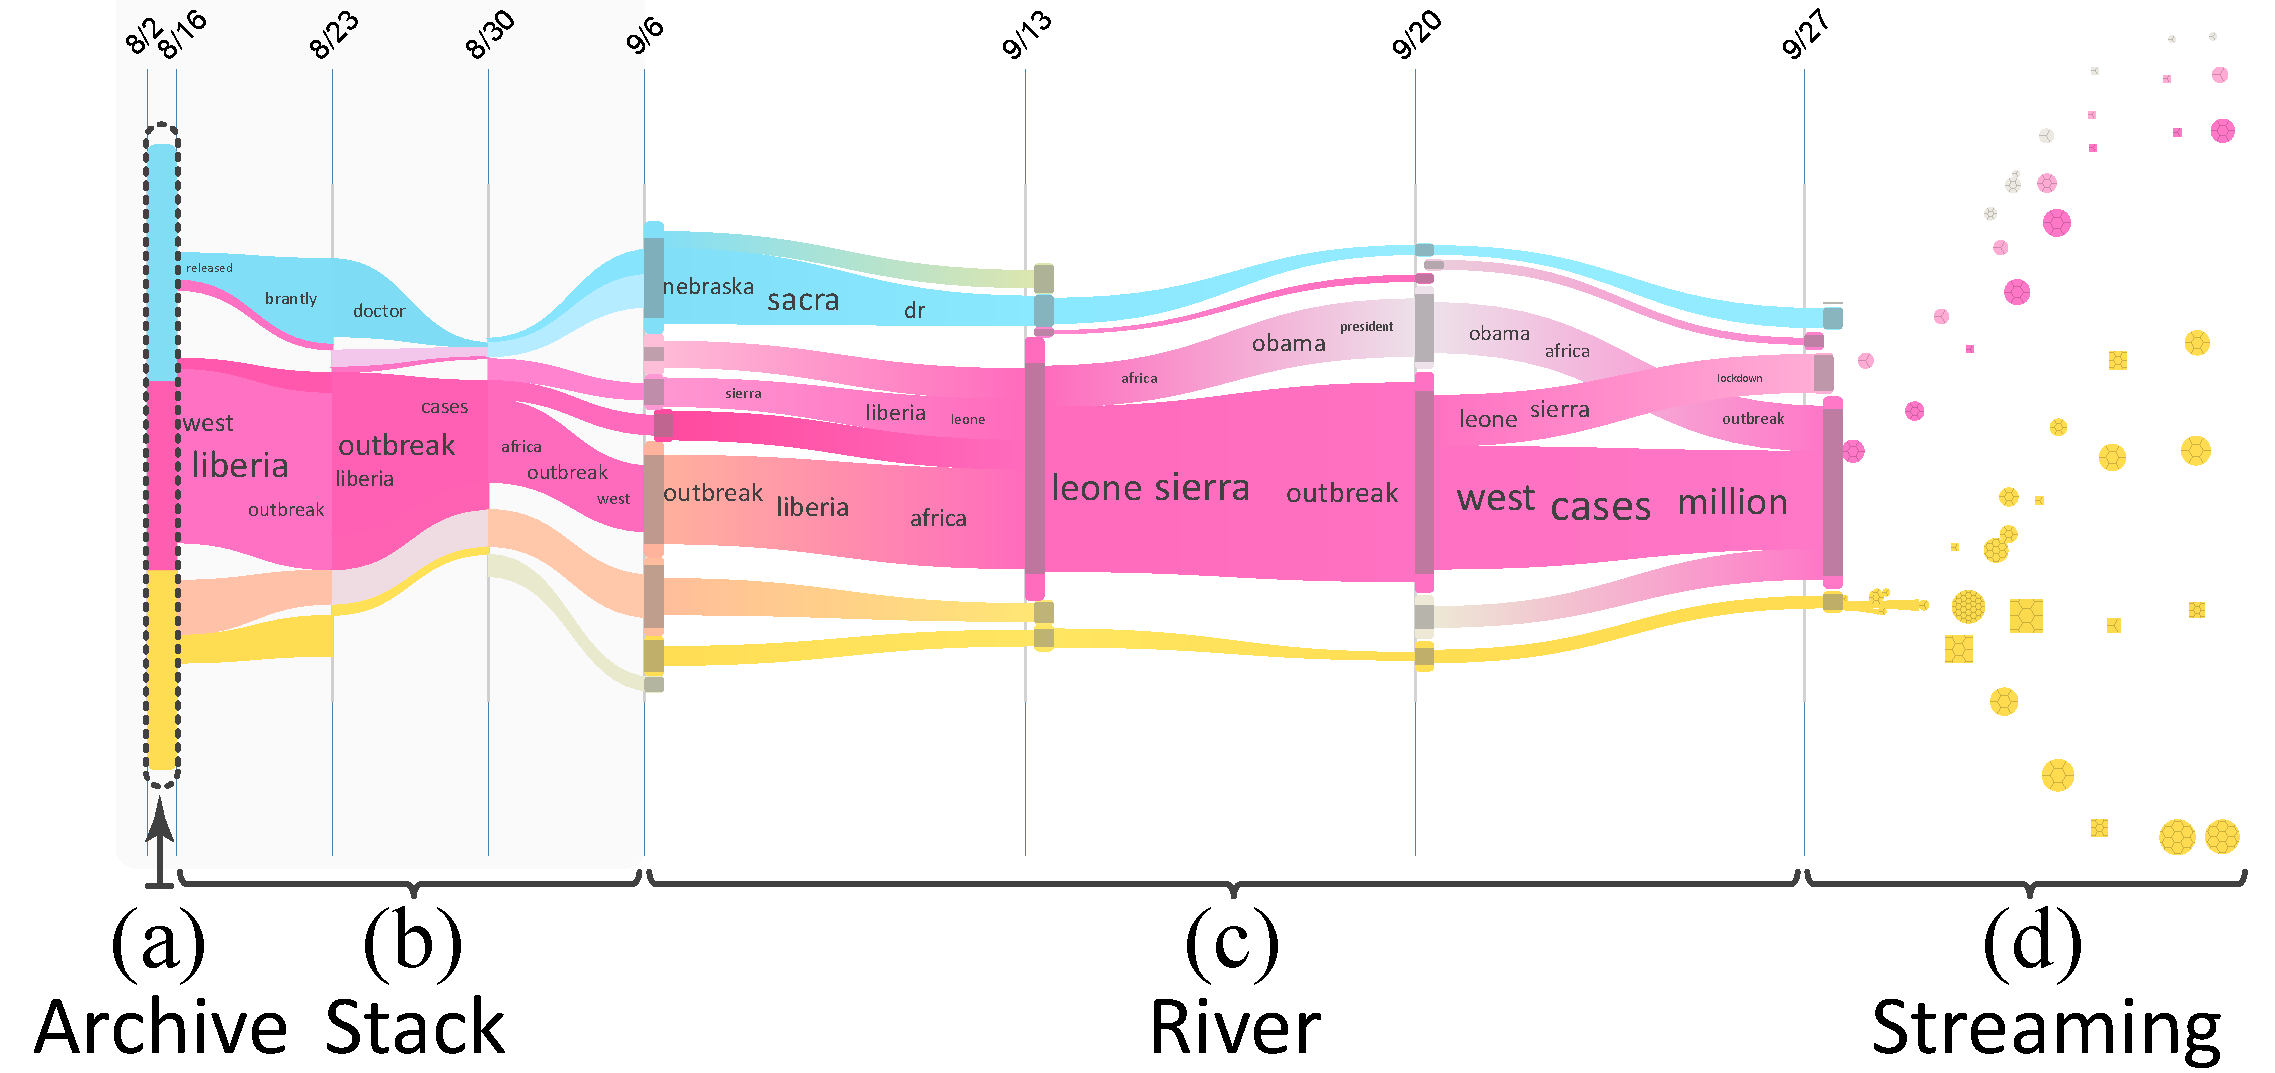
\includegraphics[width=\columnwidth]{fig/fourAreas}
	\vspace{-4mm}
	\caption{The visualization is divided into four areas: (a) archive; (b) stack; (c) river; (d) streaming.}
    %\vspace{-5mm}
	\label{fig:fourAreas}
\end{figure}

\subsection{Visualization Overview}

%Based on the guidelines described in Sec.~\ref{sec:rationale}, we design the \emph{\normalsize TopicStream} visualization (Fig.~\ref{fig:fourAreas}).
Based on the guidelines described in Sec.~\ref{sec:rationale}, we \dc{designed} the \emph{\normalsize TopicStream} visualization (Fig.~\ref{fig:fourAreas}).
%We design the \emph{\normalsize TopicStream} visualization, which is shown in Fig.~\ref{fig:fourAreas}, \kg{based on the guidelines described in Sec.~\ref{sec:rationale}, }.
The \emph{\normalsize x}-axis represents time.
The cut nodes are visualized as vertical bars at the corresponding time step.
The evolutionary relationship between cut nodes is represented by the stripes between the corresponding vertical bars.
%The flowing dots on the right side represents the newly arrived documents that are currently streaming in.
The flowing dots on the right side \kg{represent} the newly arrived documents that are currently streaming in.
%The different colors encodes different topics.
The different colors encode \kg{various} topics.\looseness=-1

%The core interest of our visualization is to help users track the dynamic characteristics of text streams.
The core \dc{intent} of our visualization is to help users track the dynamic characteristics of text streams.
%Every detail in our design is carefully crafted to cater for this purpose.
%Every detail in our design is carefully crafted to cater \kg{to} this purpose.
Every detail in our design \dc{was} carefully crafted to cater \kg{to} this purpose.
%For example, sedimentation animation is used to merge newly arrived documents into the dominant center of the visualization (\textbf{R2}).
%For example, sedimentation animation is used to merge newly arrived documents \kg{in} the dominant center of visualization (\textbf{R2}).
For example, sedimentation animation is used to merge newly arrived documents \kg{in} the dominant center of \dc{the} visualization (\textbf{\normalsize R2}).
% and gradually merge them with exiting topics.
%When more and more documents arrive, topic bars will gradually move to the other side of the display and leave more space for new topics (\textbf{R1}).
\kg{As the number of arriving documents increases}, topic bars gradually move to the other side of the display and leave \kg{a} space for new topics (\textbf{\normalsize R1}).
%With this mechanisms, users can more focus on the latest development of topics and find interesting patterns to conduct further analysis.
%With \kg{such} mechanisms, users can focus on the latest development of topics and \kg{identify} interesting patterns to conduct further analysis.
With \kg{such} mechanisms, users can focus on the latest development of topics and \kg{identify} interesting patterns to conduct further analysis.
%Specifically, the visualization consists of four regions (Fig.~\ref{fig:fourAreas}, \textbf{R1}):
\kg{In particular,} the visualization consists of four regions (Fig.~\ref{fig:fourAreas}, \textbf{\normalsize R1}):\looseness=-1
\begin{enumerate}
%\item \textbf{Stack}, which is next to the archive region and contains the older topics and documents that are compressed together due to the limited screen space;

\item \textbf{\normalsize Streaming}, which is on the rightmost side of \dc{the} visualization\kg{,} consists of newly streamed-in documents (e.g., the time period after Sep. 27  in Fig.~\ref{fig:fourAreas}(d)).

\item \textbf{\normalsize River}, which is the dominant region of \dc{the} visualization\kg{,} consists of recent topics \kg{along with} their splitting and merging relationships (e.g., Sep. 6 - 27 in Fig.~\ref{fig:fourAreas}(c)).

\item \textbf{\normalsize Stack}, which is to the left of the river region\kg{,} contains older topics and documents (e.g., Aug. 16 - Sep. 6 in Fig.~\ref{fig:fourAreas}(b)).
To reduce the visual complexity caused by the splitting and merging relationships, this region removes splitting/merging branches and only displays the mainstream of each topic.
Since users want to keep track of how the topics in this region connected with the topics in the river region, the white spaces between the topic stripes are not removed.
The width of each time step in this region is smaller than that in the river region to save space.\looseness=-1

\item \textbf{\normalsize Archive}, which is on the leftmost side, contains the oldest topics and documents (e.g., Aug. 2 - 16 in Fig.~\ref{fig:fourAreas}(a)).
 %that are compressed together \kg{because of} the limited screen space.
%Although the stacked region can save a certain amount of space, it is still cluttered for a text stream with tens or even hundreds of time steps.
Although the stacked region can \docpr{reduce the} amount of space \docpr{required}, it is still cluttered for a text stream with tens or even hundreds of time steps.
To solve this issue, we introduce the archive region,
which uses a stacked bar (Fig.~\ref{fig:fourAreas}(a)) to represent documents whose times are \emph{\normalsize k} time steps earlier than the newly streamed-in ones.
In \emph{\normalsize TopicStream}, \emph{\normalsize k} is specified by the user.
For example, \emph{\normalsize k} is set to 8 in the example of Fig.~\ref{fig:fourAreas}.
%To allocate more space for the recent documents as well as keep historical information in context, a bar region is used to encode documents whose times are \emph{\normalsize k} time steps earlier than the recent ones.
%In \emph{\normalsize TopicStream}, \emph{\normalsize k} is set by the user.
%For example, in the Ebola dataset, \emph{\normalsize k} is set to 7 by the expert.
To save space, the width of the bar is fixed no matter how many documents are archived.
Each bar item represents a topic.
Its height represents the average number of documents of each time step that belongs to this region.
%When a user examines the historically relevant documents, this region will be expanded as a stack graph with packed documents (Fig.~\ref{fig:dochighlight}).

%\item \textbf{River}, which is the dominant region of the visualization and consists of the recent topics and their splitting and merging relationships;
%\item \textbf{River}, which is the dominant region of visualization\kg{,} consists of recent topics \kg{along with} their splitting and merging relationships; \kg{and}

%\item \textbf{Streaming}, which is on the rightmost side of the visualization and consists of the newly streamed-in documents.
%\item \textbf{Streaming}, which is on the rightmost side of visualization\kg{,} consists of newly streamed-in documents.

\end{enumerate}
%The visual design of the archive and stack regions are quite straightforward. In this section, we will introduce the visual design of the river and streaming regions in detail.
%As described above, the archive and stack regions employ a bar and a stacked graph to show the corresponding topics.
%As described above, the visualization designs of a bar and a stacked graph are quite straightforward.
As described above, the visualization designs \docpr{for} a bar and a stacked graph are quite straightforward.
%We then introduce the visualization \kg{designs} of the river and streaming regions in detail.
We \docpr{will next} introduce the visualization \kg{designs} of the river and streaming regions in detail.

%The visual encodings used in our system are illustrated below.

\subsection{Visualization Design}
%\subsubsection{Tree Cut as River}
\subsubsection{Tree Cut as \kg{a} River}

\noindent\textbf{\normalsize Visual Encoding.}
%As in~\cite{cui2014}, each cut node is represented by a vertical bar (topic bar).
Each cut node is represented by a vertical bar (topic bar) \kg{similar to that presented in~\cite{cui2014}.}
The tree depth of a cut node is represented by the horizontal offset to the time step.
%The deeper a node in the tree, the further the corresponding topic bar moved to the right.
\kg{When} a node in the tree \kg{is deep}, the corresponding topic bar \kg{moves} to the right.

%The number of documents contained by a topic node is represented by the height of the topic bar.
The number of documents contained \kg{in} a topic node is represented by the height of the topic bar.
The width of the colored stripe between two topic bars indicates the number of document pairs between the two bars.
For example, the left width of the stripe represents the portion of documents mapped to the documents in the right topic bar.
%The dark region in the middle of a topic bar represents the portion of documents mapped to the documents both in the previous and next topic trees.
The dark region in the middle of a topic bar represents the portion of documents mapped to the documents both in the previous and \kg{the} next topic trees (Fig.~\ref{fig:fourAreas}).


\noindent\textbf{\normalsize Layout.}
%The basic representation of the visualization is a directed acyclic graph (DAG).
The basic representation of the visualization is a directed acyclic graph (DAG).
%A node represents a topic, and an edge between nodes encodes the evolutionary relationships between topics with mapping.
A node represents a topic and an edge between nodes encodes the evolutionary relationships between topics with mapping.
%When a new batch of documents are processed, we first run the DAG layout algorithm to find an optimal order for the new topic nodes.
When a new batch of documents \kg{is} processed, we first run the DAG layout algorithm to \kg{determine} an optimal order for the new topic nodes.
Once the topological structure is computed,  a force model is built to generate the sedimentation animation and merge new documents with existing topic bars.

\begin{figure}[t]
  \centering
  % \rule{2cm}{2cm}
 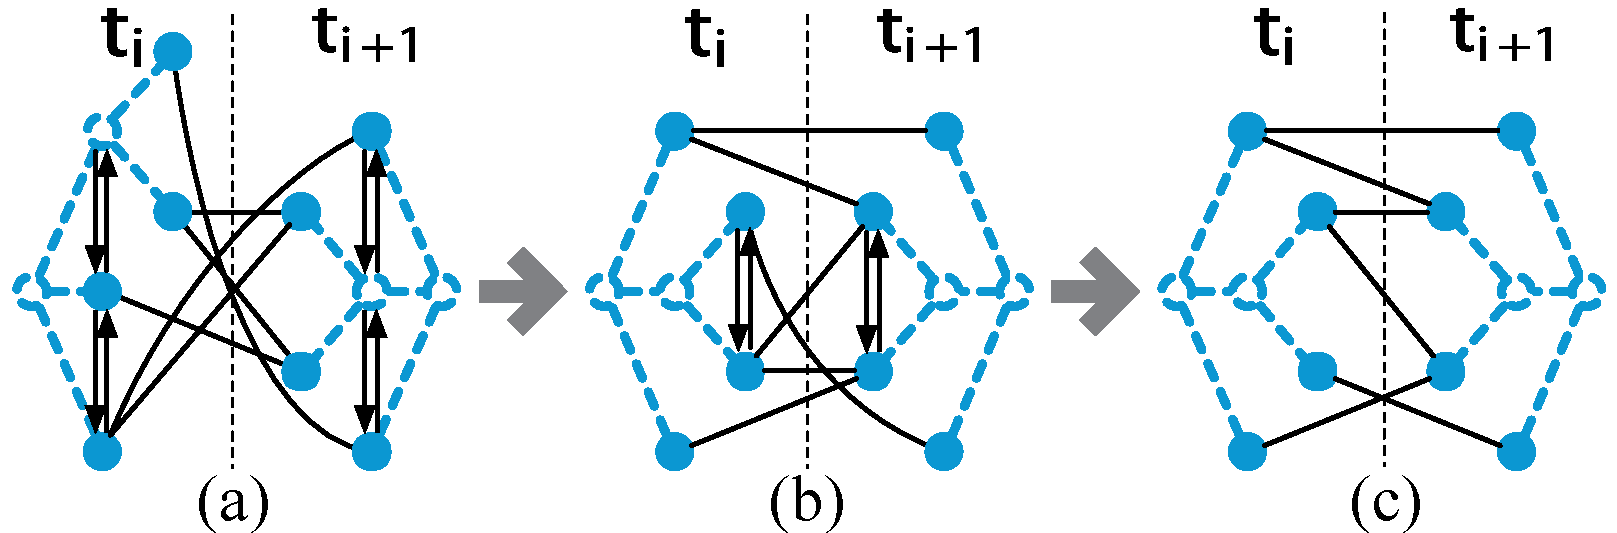
\includegraphics[width=\columnwidth]{fig/reorder}
 \vspace{-3mm}
  \caption{
%  \small
%  Example of reordering in levels: (a) reorder level one; (b) reorder level two; (c) result.
Reordering example: (a) reorder level one; (b) reorder level two; (c) result.
}
  \label{fig:reorder}
  \vspace{-1mm}
\end{figure}

\begin{figure}[t]
  \centering
  % \rule{2cm}{2cm}
 
\includegraphics[width=3in]{fig/route}
 %\vspace{-3mm}
  \caption{
  %Example of edge routing: (a) the stripe is hidden by the topic bar; (b) two more intermediate points are added; (c) a B\'{e}zier curve is utilized to improve the visual quality.
  Example of edge routing: (a) the stripe is hidden by the topic bar; (b) two intermediate points are added; (c) a B\'{e}zier curve is utilized to improve visual quality.
  }
  \label{fig:route}
  \vspace{-5mm}
\end{figure}


%\subsubsection{Reordering and Edge Routing}

%To generate a legible layout and better illustrate the evolving patterns, we first reorder the cut nodes at each time point to minimize edge crossings between neighboring time points, then route edges to avoid overlapping between nodes and edges, and finally representative documents on a selected stripe.
We \kg{initially} reorder the cut nodes at each time step to minimize edge crossings between neighboring time steps \kg{and generate a legible layout that illustrates the evolving patterns.} \kg{Edges are then routed} to avoid overlapping between nodes and edges. \kg{Finally}, representative documents \kg{are packed} on a selected stripe.

%\emph{\normalsize Reordering.} Sugiyama's heuristics~\cite{Sugiyama1981}, a well-known DAG layout algorithm, is employed to reorder the nodes at each time to minimize edge crossings.
\emph{\normalsize Reordering.} Sugiyama's heuristics~\cite{Sugiyama1981}, \kg{which is} a well-known DAG layout algorithm, is employed to reorder the nodes at each time step to minimize edge crossings.
%However, if we directly run the algorithm without constraints, the sibling nodes may be separated by other nodes.
However, if we directly run the algorithm without constraints, sibling nodes \kg{can} be separated by other nodes.
%To ensure that the sibling nodes stay together, we implement Sugiyama's heuristics from the top to the lowest level of the tree at each time.
%We implement Sugiyama's heuristics from \kg{highest} to the lowest \kg{levels} of the tree at each time \kg{to ensure that the sibling nodes stay together}
We implement Sugiyama's heuristics from \dc{the} \kg{highest} to the lowest \kg{levels} of the tree at each time \kg{to ensure that the sibling nodes stay together}\dc{.}
%The sibling nodes with the same parent are regarded as a compound node.
%At each level, we first reorder the sibling nodes inside each compound node, then sort the compound nodes accordingly.
Fig.~\ref{fig:reorder} provides an example generated by the reordering algorithm.

%\emph{\normalsize Edge Routing.} The stripes and topic bars may overlap because the topic nodes are offset to encode their depth (Fig.~\ref{fig:route}(a)).
\emph{\normalsize Edge Routing.} \kg{Stripes} and topic bars \kg{can} overlap because topic nodes are offset to encode their depth (Fig.~\ref{fig:route}(a)).
We employ the edge routing technique~\cite{Cui2008} to solve this problem.
Two additional intermediate points are introduced for each overlapping part to route the stripe.
%Two additional intermediate points are introduced for each overlapping \docpr{section} to route the stripe and avoid overlapping.
The B\'{e}zier curve is utilized to help users follow the striped path (Fig.~\ref{fig:route}).

\begin{figure}[t ]
  \centering
  % \rule{2cm}{2cm}
  \vspace{-3mm}
 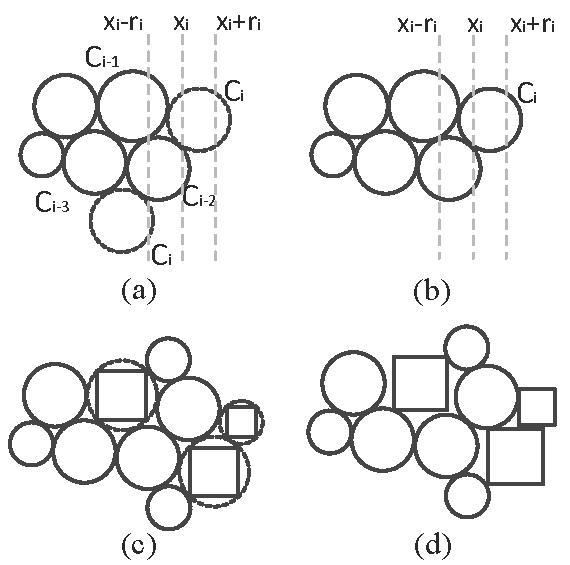
\includegraphics[width=0.7\linewidth]{fig/packing}
 \vspace{-1mm}
  \caption{
  %Illustration of the packing algorithm: (a) find possible placement positions of $C_i$; (b)set the position closest to ($x_i$, 0) as the placement position; (c) replace some circles by the corresponding rectangles; (d) reduce the gap with the size constraint and derive the final packing result.
  Illustration of the packing algorithm:
  (a) \kg{finding} possible placement positions of $C_i$;
  (b) \kg{setting} the position closest to ($x_i$, 0) as the placement position;
  (c) \kg{replacing several} circles \kg{with} the corresponding squares;
  %(d) \kg{reducing} the gap with the size constraint and \kg{deriving} the final packing result.\looseness=-1
  (d) \kg{reducing} the gap with the size \docpr{constraints} and \kg{deriving} the final packing result.\looseness=-1
  }
  \label{fig:packing}
  \vspace{-3mm}
\end{figure}

\begin{figure}[b]
  \centering
  \vspace{-3mm}
 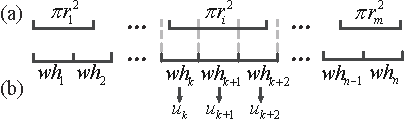
\includegraphics[width=2.6in]{fig/packposition3}
  \caption{
  %Derivation of the initial \emph{x} position.
  \kg{Deriving} the initial \emph{x} position:
  (a) align all the circles on a straight line based on their areas;
  (b) align all the stripe segments on a straight line based on their areas.
  %The dotted vertical lines indicate the overlapping relationship the area of the circle and that of the segmented stripes.
  The dotted vertical lines indicate the overlapping relationship \docpr{between} the area of the circle and that of the segmented stripes.
%Based on the relationship, $\normalsize x_i$ is approximated by $\normalsize average(u_k, u_{k+1}, u_{k+2})$.
  Based on \docpr{this} relationship, $\normalsize x_i$ is approximated \docpr{as an} $\normalsize average(u_k, u_{k+1}, u_{k+2})$.
  }
  \label{fig:xvalue}
\end{figure}

%\begin{figure}[t]
%  \centering
%  % \rule{2cm}{2cm}
%%  \vspace{-3mm}
% 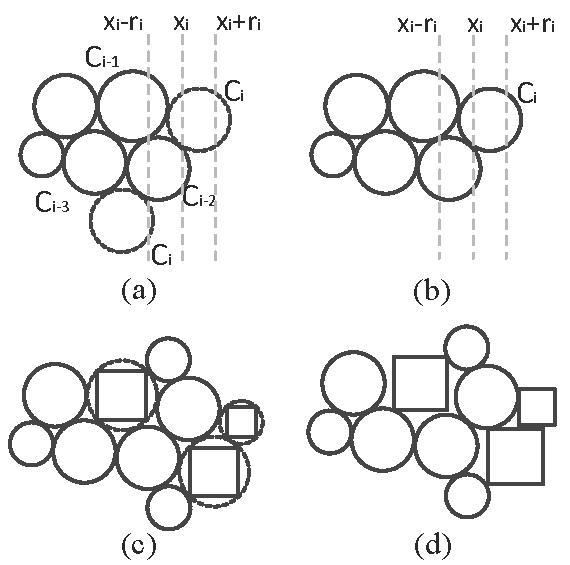
\includegraphics[width=0.7\linewidth]{fig/packing}
% \vspace{-2mm}
%  \caption{
%  %Illustration of the packing algorithm: (a) find possible placement positions of $C_i$; (b)set the position closest to ($x_i$, 0) as the placement position; (c) replace some circles by the corresponding rectangles; (d) reduce the gap with the size constraint and derive the final packing result.
%  Illustration of the packing algorithm: (a) \kg{finding} possible placement positions of $C_i$; (b) \kg{setting} the position closest to ($x_i$, 0) as the placement position; (c) \kg{replacing several} circles \kg{with} the corresponding rectangles; (d) \kg{reducing} the gap with the size constraint and \kg{deriving} the final packing result.}
%  \label{fig:packing}
%  \vspace{-3mm}
%\end{figure}



%\emph{\normalsize Packing}. To help users understand and compare the relationships between documents, including the coming order and similarity relationships, we pack them on the topic stripe (\textbf{R3}).
\emph{\normalsize Packing}. We pack \kg{the documents} on the topic stripe %(\textbf{\normalsize R3}) \kg{to help users understand and compare their relationships, including incoming order and similarity relationships.}
(\textbf{\normalsize R3}) \kg{to help users understand and compare their relationships, \docpr{including the incoming} order and similarity relationships.}
%In our visualization, each news article cluster is represented by a circle, while each Twitter cluster is represented by a rectangle.
Each news article is represented by a circle \kg{in our visualization}, \kg{whereas} each tweet is represented by a square.
%For simplicity, each rectangle is approximately represented by a circle whose center is that of the rectangle and whose radius is $\beta\cdot\sqrt{2}a$.
For \dc{the sake of} simplicity, each square is approximately represented by a circle whose center is \dc{the same as} the square\dc{'s} and whose radius is $\beta\cdot\sqrt{2}b$.
%Each rectangle is approximately represented by a circle whose center is \kg{that} of the rectangle and whose radius is $\beta\cdot\sqrt{2}a$ \kg{for simplicity}.
%Here $a$ is the side length of the rectangle and $\beta$ ($1\leq\beta\leq1/\sqrt{2}$) is a parameter to balance the intersection and gap between the elements (e.g., circles and rectangles) in the final packing result.
%$a$ is the side length of the rectangle and $\beta$ ($1\leq\beta\leq1/\sqrt{2}$) is a parameter \kg{that balances} intersection and gap\kg{s} between elements (e.g., circles and rectangles) in the final packing result.
%$b$ is the side length of the rectangle and $\beta$ ($1\leq\beta\leq1/\sqrt{2}$) is a parameter \kg{that balances} \dc{the} intersection and gap\kg{s} between elements (e.g., circles and rectangles) in the final packing result.
$\normalsize b$ is the side length of the square and $\beta$ ($1/\sqrt{2}\leq\beta\leq1$) is a parameter \kg{that balances} \dc{the} intersection and gap\kg{s} between elements (e.g., circles and squares) in the final packing result.
%The larger $\beta$ is, the more gap might be.
The larger $\beta$ is, the \dc{larger the} gap might be.
%This transformation preserves the area enclosed by the boundary.
%With this approximation, the packing problem is formulated as a circle packing problem.
The packing problem is formulated as a circle packing problem \kg{using this approximation}.
%We then employ a front-chain-based circle packing algorithm as in~\cite{Wang2006visualization,ZhaoTVCG2014} to tightly pack circles on the selected stripe.
%We then employ a front-chain-based circle packing algorithm as in~\cite{Wang2006visualization,ZhaoTVCG2014} to pack circles \kg{tightly} on the selected stripe.
We then employ a front-chain-based circle packing \docpr{algorithm, as in~\cite{Wang2006visualization,ZhaoTVCG2014}, to} pack circles \kg{tightly} on the selected stripe.
%Fig.~\ref{fig:packing} illustrate the basic idea of this packing algorithm.
Fig.~\ref{fig:packing} illustrate\kg{s} the basic idea of this packing algorithm.
%Fig.~\ref{fig:packing} illustrate\kg{s} the basic \docpr{concept} of this packing algorithm.

%Compared with the packing problem described in~\cite{ZhaoTVCG2014}, ours does not provide the initial \emph{x}-coordinate for each circle.
Compared with the packing problem described in~\cite{ZhaoTVCG2014}, our \kg{problem} does not provide the initial \emph{x} coordinate for each circle.
%In our packing problem, only the coming order of each circle is provided.
Only the incoming order of each circle is provided in our packing problem.
%Thus, we need to derive the initial \emph{x}-coordinate based on the order of circles.
Thus, we \kg{have} to derive the initial \emph{x} coordinate based on the order of \kg{the} circles.
%The basic idea is to find an approximate placement position of each circle, which is achieved by approximately mapping its area to the area of the segmented stripes in ascending order.
The basic idea is to \kg{determine} an approximate placement position \kg{for} each circle, which is achieved by approximately mapping its area to the area of the segmented stripes.
%Then the averaged x-coordinates of the corresponding segmented stripes is used to approximate the initial x-coordinate of the circle.
%The averaged \emph{x} coordinates of the corresponding segmented stripes is \kg{then} used to approximate the initial \emph{x} coordinate of the circle.
The average \dc{of the} \emph{x} coordinates of the corresponding segmented stripes is \kg{then} used to approximate the initial \emph{x} coordinate of the circle.
%Specifically, we align all the circles on a straight line based on their areas (Fig.~\ref{fig:xvalue}(a)).
\kg{In particular}, we align all the circles on a straight line based on their areas (Fig.~\ref{fig:xvalue}(a)).
The area of circle $C_i$ is $\pi{r_i}^2$.
%For simplicity, we denote it by ${r_i}^2$.
%Next, we divide the stripe into \emph{\normalsize n} uniform segments along its \emph{x}-axis.
We \kg{then} divide the stripe into \emph{\normalsize n} uniform segments along its \emph{x}-axis.
The height of the \emph{\normalsize k}-th segment is denoted as $h_k$ and its area is $wh_k$,
%Here $w$ is the width of each segment along the \emph{x}-axis.
\kg{where} $w$ is the width of each segment along the \emph{x}-axis.
All these segments are also aligned on a straight line based on their areas (Fig.~\ref{fig:xvalue}(b)).
%As shown in Fig.~\ref{fig:xvalue}, with these two straight lines, the overlapping relationship between the area of the circle and that of the segmented stripes can be discovered.
Fig.~\ref{fig:xvalue} \kg{shows that} the overlapping relationship between the area of the circle and that of the segmented stripes can be \kg{determined using two straight lines}.
%For example, in this figure, the initial $x_i$ is approximated by $average(x_k, x_{k+1}, x_{k+2})$.
%For example, the initial $x_i$ in this figure is approximated by $average(x_k, x_{k+1}, x_{k+2})$.
For example, the initial $x_i$ of circle \emph{\normalsize i} in this figure is approximated by $\normalsize average(u_k, u_{k+1}, u_{k+2})$.
Here $u_k$ is the \emph{x} coordinate of the center of \emph{\normalsize k}-th segment.

\noindent \textbf{\normalsize Interaction}.
%In addition to the interactions described in~\cite{cui2014}, such as details on demand, collapsing/expanding time points, splitting/merging topic bars, and changing focus, we also provide the following interactions to explore the complex evolutionary clustering results from multiple perspectives.
%We also provide the following interactions to explore the complex evolutionary clustering results from multiple perspectives \kg{aside from the interactions described in~\cite{cui2014} (e.g. details on demand, collapsing/expanding time points, splitting/merging topic bars, and changing focus).}
%We also provide the following interactions to explore the complex evolutionary clustering results from multiple perspectives \kg{aside from the interactions described in~\cite{cui2014} (e.g. details on demand, collapsing/expanding time steps, splitting/merging topic bars, and changing focus).}
We also provide the following interactions to explore the complex evolutionary clustering results from multiple perspectives \kg{\docpr{in addition to} the interactions described in~\cite{cui2014} (e.g. details on demand, collapsing/expanding time steps, splitting/merging topic bars, and changing focus).}

\emph{\normalsize Document Query}.
%Once the tokens have transformed into a colored stripe, we adopt voronoi treemap~\cite{} to encode the containing documents within the color stripe for further query and analysis.
Once the documents \kg{are} transformed into a colored stripe, we adopt \kg{circle packing} to encode the documents \kg{contained} within the color stripe for further query and analysis.
%In the example shown in  Fig.~\ref{fig:vtreemap}, users can click the stripe and turn it into a treemap, in which thicker borders indicate tokens while the thin borders indicate documents contained by each token.
%The example in  Fig.~\ref{fig:vtreemap} \kg{shows that} users can click the stripe and turn it into a circle/rectangle packing, in which a circle represents a news article \kg{whereas} the rectangle encodes a tweet.
The example in  Fig.~\ref{fig:vtreemap} \dc{shows how} users can click the stripe and turn it into a circle/square packing, in which a circle represents a news article \dc{and a} square encodes a tweet.
%From this figure, we can easily see the number of tokens that sediment to this topic and compare their relative size.
%\kg{This} figure \kg{shows} the number of tokens that sediment \kg{into} this topic and compare\kg{s} their relative size\kg{s}.
%Once the packing result is displayed, users can manually click one or more document to examine their content in detail.
Once the packing result is displayed, users can manually click one or more \dc{documents} to examine \dc{the} content in detail.

\emph{\normalsize Visual Comparison}.
%By leveraging circle packing algorithm, we allow users to compare the relationships among different time points.
%We allow users to compare the relationships among different time points \kg{by leveraging circle packing algorithm.}
We allow users to compare the relationships among different time steps by leveraging \dc{a} circle packing algorithm.
%For example, users can compare the incoming order and similarity relationships in Fig.~\ref{fig:ebola}(a) and in Fig.~\ref{fig:ebola}(b).
%For example, users can compare the incoming order and similarity relationships Fig.~\ref{fig:ebola}(a) and Fig.~\ref{fig:ebola}(b).
For example, users can compare the incoming order and similarity relationships\docpr{, as shown in} Fig.~\ref{fig:ebola}(a).
%One of our experts, professor P2 commented, ``Comparing the incoming order of documents help me easily discover who talk a topic first (set the agenda) and who follows immediately.
%One of our experts, P2, commented \kg{that}, ``Comparing the incoming order of documents \dc{helps} me easily discover who \kg{talked about} a topic first (\kg{that is, who} set the agenda) and who follow\kg{ed} immediately.
One of our experts, P2, commented \kg{that}, ``Comparing the incoming order of documents \dc{helps} me easily discover who \kg{talked about} a topic first (\kg{that is, who} set the agenda) and who \docpr{immediately follow\kg{ed}}.
%This \kg{feature} is useful \kg{to study} agenda setting in my field.''
This \kg{feature} \dc{can help me} \kg{study} agenda setting in my field.''

\subsubsection{Streaming Document as Sedimentation}

%\begin{figure}[t]
%  \centering
% 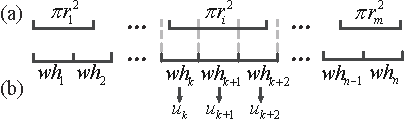
\includegraphics[width=2.6in]{fig/packposition3}
%  \caption{
%  %Derivation of the initial \emph{x} position.
%  \kg{Deriving} the initial \emph{x} position: (a) align all the circles on a straight line based on their areas; (b) align all the stripe segments on a straight line based on their areas. The dotted vertical lines indicate the overlapping relationship the area of the
%circle and that of the segmented stripes. Based on the relationship, $\normalsize x_i$ is approximated by $\normalsize average(u_k, u_{k+1}, u_{k+2})$.
%  }
% \vspace{-3mm}
%  \label{fig:xvalue}
%\end{figure}

\begin{figure}[b]
	\vspace{-3mm}
	\centering
	\includegraphics[width=\columnwidth]{fig/vtreemap}
	\vspace{-5mm}
	\caption{
	%Encode documents after sedimentation as a \kg{circle/square packing}.
	Encode documents after sedimentation \docpr{as \kg{circle/square packing}}.
	}
	\label{fig:vtreemap}
%	\vspace{-3mm}
\end{figure}


\noindent \textbf{\normalsize Visual Encoding}.
%Inspired by visual sedimentation~\cite{Huron2013visual}, we use the river sedimentation metaphor to encode the process of newly arrived text documents merging with existing topics (\textbf{R2}).
Inspired by visual sedimentation~\cite{Huron2013visual}, we use the river sedimentation metaphor to encode the process of newly arrived text documents \kg{that merge} with existing topics (\textbf{\normalsize R2}).
To quicken the sedimentation process of a high-volume text stream, a set of document clusters are derived from the incoming documents by using k-means clustering.
A token is a visual mark representing a document cluster.
%The generation process of the sedimentation metaphor consists four steps:
The generation process of the sedimentation metaphor consists \dc{of} four steps:

\emph{\normalsize Entrance}.
%Newly arrived documents are represented as circular or rectangular tokens (Fig.~\ref{fig:fourAreas}) and flying into the view from the right hand side.
Newly arrived documents are represented as circular or rectangular tokens (Fig.~\ref{fig:fourAreas}) \kg{that come} into view from the right side.
%To handle the scalability issue, documents of similar content are clustered into one token, the size of which indicates the document number.
Documents \kg{with} similar content are clustered into one token, the size of which indicates the \kg{number of} documents, \kg{to handle the scalability issue}.
The color of each token encodes the topic that it contains.

\emph{\normalsize Suspension}.
%Each token will fly towards (from right to left) the corresponding topic bars of the latest time point.
Each token \kg{moves toward} (from right to left) the corresponding topic bars of the latest time step.
%During the movement, the sizes of tokens will decrease gradually.
%\kg{Token sizes} decrease gradually \kg{during the movement}.
Token \dc{size} \dc{decreases} gradually \kg{during the movement}.

\emph{\normalsize Accumulation} and \emph{\normalsize decay}.
%Once tokens touch the corresponding topic bars or other tokens that have already settled, they will stop moving and begin to shrink (decay).
\kg{The tokens} will stop moving and start \kg{to} decay \kg{once they touch the corresponding topic bars or other tokens that have already settled.}
%The settled tokens will continue to .
The settled tokens continue to shrink and merge \kg{with} existing topics.

\emph{\normalsize Aggradation}.
%When the settled tokens resolve, the colored stripes continue to grow and indicates the latest development of news topics.
The colored stripes continue to grow and \kg{indicate} the latest development of topics \kg{when the settled tokens are resolved}.

%Once a batch of news documents (e.g., for a day) are all sedimented, corresponding topic bars will appear, and push older topic bars to the left hand side.
%Once a batch of news documents (e.g., for a day) are all sedimented, \kg{the} corresponding topic bars appear and push older topic bars to the hand side.
%Once a batch of documents (e.g., for a day) are all sedimented, \kg{the} corresponding topic bars appear and push older topic bars to the \dc{left-hand} side.
Once a batch of documents (e.g., for a day) \docpr{are sedimented}, \kg{the} corresponding topic bars appear and push older topic bars to the \dc{left-hand} side.
%The achieve and the stack regions will change accordingly.
The archive and stack regions \kg{then} change accordingly.

\begin{figure}[t]
	\centering
	\includegraphics[width=\columnwidth]{fig/docHighlight}
	\vspace{-4mm}
%	\caption{Relevant documents of cluster A are highlighted in both the river (B) and the archive (C) regions.\looseness=-1}
	\caption{
	%Relevant documents of cluster A are highlighted in both the river (B)\xiting{, the stack (C),} and the archive (\xiting{D}) regions.\looseness=-1
	Relevant documents of cluster A are highlighted \docpr{in the} river (B)\xiting{, the stack (C),} and the archive (\xiting{D}) regions.\looseness=-1
	}
\vspace{-5mm}
	\label{fig:dochighlight}
\end{figure}

\noindent \textbf{\normalsize Layout}.
%During the sedimentation process, each token is given a region based on the topological structure in the ``reordering and edge routing'' step.
Each token is \kg{assigned to} a region based on the topological structure in the ``reordering and edge routing'' step \kg{during the sedimentation process.}
%The token can only move within the given region, and cannot cross the border.
%The token can only move within the \kg{assigned to} region, and cannot cross the border.
The token can only move within the \dc{assigned region} and cannot cross the border.
%The moving speed of the token is controlled by two forces: 1) a universal gravity force and 2) an attractive force between the moving token and the tokens that are already sedimented.
%The moving speed of the token is controlled by two forces: 1) a universal gravity force and 2) an attractive force between the token and the \kg{sedimented} tokens.
The \dc{speed} of the token is controlled by two forces: 1) a universal gravity force and 2) an attractive force between the token and the \kg{sedimented} tokens.
%The gravity force provides each token a constant acceleration from right to left.
The gravity force provides each token \kg{with} constant acceleration from right to left.
%The attractive force ensures that similar documents will sediment close to each other.
The attractive force ensures that similar documents will sediment close to \kg{one another.}
Therefore, the total acceleration $a_k$ for a moving token $k$ is defined as
$$a_k=g+\sum_is_{ik}*{n_i}/{||p_i-p_k||^2},$$
%where $g$ is the constant gravity acceleration, $p_i$ is the location of token $i$ that is already sedimented, $p_k$ is the location of token $k$, $m_i$ is the number of documents in token $i$, and $s_{ik}$ is the content similarity between token $i$ and $k$.
where $g$ is the constant gravity acceleration, $p_i$ is the location of \kg{sedimented} token $i$, $p_k$ is the location of token $k$, $n_i$ is the number of documents in token $i$, and $s_{ik}$ is the content similarity between token\kg{s} $i$ and $k$.


%\noindent \textbf{\normalsize Interaction}
\noindent \textbf{\normalsize \xiting{Interaction.}}
%The sedimentation visualization also to allow users to interactively examine the content of new coming documents and compare them with the older documents.
%The sedimentation visualization also allow\kg{s} users to examine the content of \kg{incoming} documents \kg{interactively} and compare them with older documents.
The sedimentation visualization also allow\kg{s} users to examine the content of \docpr{the} \kg{incoming} documents \kg{interactively} and compare them with older documents.

\emph{\normalsize Document Link}.
%In many text stream analysis tasks, it is desired to quickly find related documents covering a long range of time period.
In many text stream analysis tasks, it is \dc{desirable} to quickly find related documents covering a long \dc{time} period.
%\kg{Finding} related documents \kg{that rapidly cover} a long range of period \kg{is the objective of many text stream analyses}.
%In our system, document highlight is supported for this need.
Document link is supported for this \kg{requirement of our system}.
%Document link is \docpr{therefore supported by} our system.
%For example, users may first explore the content in the streaming region, and find a document of interest.
For example, users \kg{can initially} explore the content in the streaming region and find a document/cluster of interest.
%Then, our system will automatically use the word vector in the given document, and locate the most similar documents in all three regions (i.e., streaming, stack, and achieve).
Our system \kg{then} automatically use\kg{s} the word vector in the given document and locate\kg{s} the most similar documents in all three regions (i.e., streaming, stack, and archive).
%Once the related documents are located, containing treemap cells or circular tokens will be automatically highlighted and connections will be displayed for users to further exploration.
Once the related documents/clusters are located, the connections \kg{are} displayed for users to \kg{explore further}.

%An example of document highlight is shown in Fig.~\ref{fig:dochighlight},
An example of document \dc{link} is shown in Fig.~\ref{fig:dochighlight},
%where a user explores the relevant documents of a new coming twitter cluster (Fig.~\ref{fig:dochighlight}A).
\kg{in which} a user explores relevant documents \kg{from an incoming Twitter} cluster (Fig.~\ref{fig:dochighlight}A).
%Relevant documents are found in both the river region (Fig.~\ref{fig:dochighlight}B)\xiting{, the stack region (Fig.~\ref{fig:dochighlight}C),} and archive region (Fig.~\ref{fig:dochighlight}\xiting{D}).
%Relevant documents are found in the river (Fig.~\ref{fig:dochighlight}B), stack (Fig.~\ref{fig:dochighlight}C), archive (Fig.~\ref{fig:dochighlight}D) \kg{regions}.
Relevant documents are found in the river (Fig.~\ref{fig:dochighlight}B), stack (Fig.~\ref{fig:dochighlight}C), \dc{and} archive (Fig.~\ref{fig:dochighlight}D) \kg{regions}.
%To felicitate the examination of the highlighted documents, the archive region is expanded accordingly.
The archive region is expanded accordingly \kg{to facilitate the examination of the relevant documents.}

%In addition, users can also click on a token while it is still in the suspension step, related documents will also be displayed for further examination.
\kg{Users} can also click on a token while it is still in the suspension step.
%Then related documents \kg{are} displayed for further examination.
\dc{Related} documents \kg{are} \dc{then} displayed for further examination.



%\section{Evaluation}\label{sec:evaluation}
%
%In this section, a quantitative evaluation of the proposed streaming tree cut algorithm is conducted.
%%The usefulness of our approach is then demonstrated with two case studies.
%The usefulness of \kg{the} approach is then demonstrated with two case studies.

%\subsection{Quantitative Evaluation}
\section{Quantitative Evaluation}
\label{sec:quantitativeevaluation}
%To assess the effectiveness of our streaming tree cut algorithm, we performed experiments on a number of different datasets.
In this section, a quantitative evaluation of the proposed streaming tree cut algorithm is conducted.

%\subsubsection{Criteria}

\subsection{Fitness and Smoothness}
%To assess the effectiveness of \kg{the} streaming tree cut algorithm, \kg{we conducted} experiments on \kg{several} datasets.
To assess the effectiveness of \kg{the} streaming tree cut algorithm, we \tvcgminor{compared our algorithm with a baseline algorithm in terms of fitness and smoothness.}

\subsubsection{Criteria}
%Fitness and smoothness were employed as two important criteria to evaluate the derived streaming tree cuts.
%The fitness measures how satisfactorily the topics on the tree cut represent the topic distribution within a topic tree.
Fitness and smoothness \kg{are} two important criteria to evaluate the derived streaming tree cuts.
\dc{Fitness} measures how satisfactorily the topics on the tree cut represent the topic distribution within a topic tree.
%The fitness measures \kg{the satisfactory representation of} the topic distribution within \kg{the topics on the tree cut}.

\noindent\textbf{\normalsize Fitness ($\bm{F}$)}:
We derived the measure from the proposed tree cut likelihood equation, $\bm{F}=p({\phi}^t|T^t)p(\mathcal{D}_{f}|{\phi}^t)$,
%\kg{The} metric from the proposed tree cut likelihood equation, $\bm{F}=p({\phi}^t|T^t)p(D_{f}|{\phi}^t)$, \kg{is derived,}
where the right side is defined in Eq.~(\ref{eq:hmm2}).
%$p({\phi}^t|T^t)$ describes how the tree cut fits the focus and $p(\mathcal{D}_{f}|{\phi}^t)$ describes how it fits the tree.
$p({\phi}^t|T^t)$ describes how the tree cut \xiting{fits} the tree and $p(\mathcal{D}_{f}|{\phi}^t)$ describes how it \xiting{fits} the focus.
%$p({\phi}^t|T^t)$ describes \kg{the fit of} the tree cut \kg{and} the focus. $p(D_{f}|{\phi}^t)$ describes \kg{the} fit \kg{of} the tree.
%The larger the $F$ value, the better the tree cut.
A larger  $F$ value \kg{indicates a} better tree cut.

%Accordingly, likelihood was utilized to measure the fitness of a tree.
%The following three metrics were introduced to assess the smoothness between adjacent tree cuts.
The following three measures \kg{assess} the smoothness between \kg{the} adjacent tree cuts.
%In our implementation, the larger the smoothness value, the smoother between two adjacent tree cuts.
In \kg{the} implementation, \kg{a} larger smoothness value \kg{means that} the two adjacent tree cuts \kg{are smoother}.



%\begin{table*}[t]
%
%\vspace{-3mm}
%    \caption{
%%    \small
%    Evaluation of the overall likelihood and smoothness.}
%    \vspace{-3mm}
%    $f_r(\cdot)=\frac{m_o-m_b}{m_b}*100\%$, where $m_b$ and $m_o$ are the measure values of the baseline method and our method.
%    \label{table:average}
%    \vspace{1mm}
%    \centering \scalebox{0.8}{
%    \begin{tabular}{|c|c|c|c|c|c|c|c|c|c|}
%
%    \hline
%    \multirow{2}{*}{Dataset}&{$f_r(\bm{F})$(\%)} & {$f_r(\bm{S_{map}})$(\%)}& \multicolumn{3}{c|}{$f_r(\bm{S_{NMI}})$(\%)} & \multicolumn{3}{c|}{$f_r(\bm{S_{dist}})$(\%)}\\
%    \cline{2-9}
%    &$F({\phi}^{t})$ & $S_{map}({\phi}^{t},{\phi}^{t-1})$ & $S_{NMI}({\phi}^{t},{\phi}^{t-1})$ & $S_{NMI}({\phi}^{t},{\phi}^{t-2})$ & $S_{NMI}({\phi}^{t},{\phi}^{t-3})$& $S_{dist}({\phi}^{t},{\phi}^{t-1})$ & $S_{dist}({\phi}^{t},{\phi}^{t-2})$&$S_{dist}({\phi}^{t},{\phi}^{t-3})$\\
%    %&$({\phi}^{t})$ & $({\phi}^{t},{\phi}^{t-1})$ & $({\phi}^{t},{\phi}^{t-1})$ & $({\phi}^{t},{\phi}^{t-2})$ & $({\phi}^{t},{\phi}^{t-3})$& $({\phi}^{t},{\phi}^{t-1})$ & $({\phi}^{t},{\phi}^{t-2})$&$({\phi}^{t},{\phi}^{t-3})$\\
%
%    \hline
%   \emph{A} & 4.5486 & 18.7873 & 7.6839 & -1.8875 & -2.6680 & 13.5781 & -1.5226 & -2.4843 \\
%    \emph{B} & 7.5084 & 26.4451 & 8.7131 & -3.1711 & -3.2452 & 13.1334 & -4.2689 & -5.4008 \\
%        \hline
%    \end{tabular}
%    }
%    \vspace{-5mm}
%\end{table*}


\noindent\textbf{\normalsize Tree mapping ($\bm{S_{map}}$)}:
%We derived the metric from the smoothness cost function of the streaming tree cut algorithm, $\bm{S_{map}}=-\sum\limits_{t}f(x_r,x_s)$,
\kg{The} measure \kg{is derived} from the smoothness cost function of the streaming tree cut algorithm, $\bm{S_{map}}(\phi^t,\phi^{t-1})=-E_2{(\phi^t,\phi^{t-1})}$,
where $E_2{(\phi^t,\phi^{t-1})}$ is defined in Eq.~(\ref{eq:hmm5}).
%The smaller the $\bm{S_{map}}$ value, the smoother between two adjacent trees.
%The following two criteria were then defined based on a metric of cluster quality and the tree structure.

%The following two criteria \kg{are} defined based on a metric of cluster quality and the tree structure.

\noindent\textbf{\normalsize Normalized Mutual Information (NMI) ($\bm{S_{NMI}}$)}:
%The NMI metric is defined as the mutual information between the cluster assignments and a pre-existing labeling.
%The NMI metric \kg{represents} the mutual information between the cluster assignments and a pre-existing \kg{label}.
The NMI measure \kg{represents} the mutual information \docpr{shared by both} the cluster assignments and a pre-existing \kg{label}.
%Hungarian algorithm~\cite{Steiglitz1982} was employed to find the optimal match between the document sets of the two tree cuts.
%Hungarian algorithm~\cite{Steiglitz1982} \kg{is} employed to find the optimal match between the document sets of the two tree cuts.
\dc{The} Hungarian algorithm~\cite{Steiglitz1982} \kg{is} employed to find the optimal match between the document sets of the two tree cuts.
%This metric assess the similarity between adjacent tree cuts.
This measure \kg{assesses} the similarity between adjacent tree cuts.
%The larger the $\bm{S_{NMI}}$ value, the smoother between two adjacent trees.


%\begin{figure*}[t]
%	\centering
%	\subfigure[Dataset \emph{A}]{\label{fig:likelihood_A}
%	\includegraphics[width=0.25\linewidth]{./fig/Likelihood_A.pdf}
%	}
%	\subfigure[Dataset \emph{B}]{\label{fig:Likelihood_B}
%\vspace{-2mm}
%	\includegraphics[width=0.25\linewidth]{./fig/Likelihood_B.pdf}
%	}
%    \subfigure[Dataset \emph{C}]{\label{fig:Likelihood_C}
%\vspace{-2mm}
%	\includegraphics[width=0.25\linewidth]{./fig/Likelihood_C.pdf}
%	}
%%\hspace{1mm}
%   \hspace{-8mm}
%   \subfigure[Legend]{\label{fig:legend}
%
%\vspace{-2mm}
%	\includegraphics[width=0.2\linewidth]{./fig/Likelihood_legend.pdf}
%	}
%%\vspace{-4mm}
%	\caption{
%%\small
%Comparison of likelihood.}\label{fig:likelihood}
%\vspace{-2mm}
%\end{figure*}




%\begin{figure*}[t]
%	\centering
%	\subfigure[Dataset \emph{A}]{\label{fig:tree_num}
%	\includegraphics[width=0.25\linewidth]{./fig/Likelihood_A.pdf}
%	}
%	\subfigure[Dataset \emph{B}]{\label{fig:Likelihood_B}
%\vspace{-2mm}
%	\includegraphics[width=0.25\linewidth]{./fig/Likelihood_B.pdf}
%	}
%    \subfigure[Dataset \emph{C}]{\label{fig:Likelihood_C}
%\vspace{-2mm}
%	\includegraphics[width=0.25\linewidth]{./fig/Likelihood_B.pdf}
%	}
%%\hspace{1mm}
%   \hspace{-8mm}
%   \subfigure[Legend]{\label{fig:legend}
%
%\vspace{-2mm}
%	\includegraphics[width=0.2\linewidth]{./fig/Likelihood_legend.pdf}
%	}
%\vspace{-4mm}
%	\caption{
%%\small
%Comparison of likelihood.}\label{fig:likelihood}
%\vspace{-2mm}
%\end{figure*}

%\begin{figure*}[b]
%\centerline
%{
%\includegraphics[width=0.235\linewidth]{./fig/Likelihood_A.pdf}
%\includegraphics[width=0.235\linewidth]{./fig/Likelihood_B.pdf}
%\includegraphics[width=0.235\linewidth]{./fig/Likelihood_B.pdf}
%\hspace{-6mm}
%\includegraphics[width=0.2\linewidth]{./fig/Likelihood_legend.pdf}
%}
%\centerline{
%Dataset \emph{A} \hspace{0.2\linewidth} Dataset \emph{B}  \hspace{0.2\linewidth} Dataset \emph{C} \hspace{0.2\linewidth} Dataset \emph{C}
%}
%\caption{Comparison of likelihood.}\label{fig:likelihood}
%\end{figure*}



\noindent\textbf{\normalsize Tree distance ($\bm{S_{dist}}$)}:
%We use this metric to measure the difference between tree cuts by aggregating the tree distance between two related cut nodes, $S_{Dist}=\log(p_{dist}(T^t|T^{k}))$ $(k=t-1, t-2, t-3)$.
%\kg{This} metric \kg{is used} to measure the difference between \kg{the} tree cuts by aggregating the tree distance between two related cut nodes, $S_{Dist}=\log(p_{dist}(T^t|T^{k}))$ $(k=t-1, t-2, t-3)$.
\kg{This} measure \kg{is used} to evaluate the difference between \kg{the} tree cuts by aggregating the tree distance between two related cut nodes \xiting{$T_s$ and $T_r$}, %\xiting{$T_s\in \mathcal{C}_{\phi^t}$ and $T_r\in \mathcal{C}_{\phi^k}$},
%$S_{Dist}=\log(p_{dist}(T^t|T^{k}))$ $(k=t-1, t-2, t-3)$.
%Here $\log p_{dist}(T^t|T^{k})$ is defined by
%\xiting{The tree distance is defined as~\cite{Wang2013}}
\xiting{
\begin{eqnarray}
\small
%\log p_{dist}(T^t|T^{k}) \triangleq  - E_{T_r,T_s\in leaves(T^t) \atop r\ne s}(D_{T^t}(T_r,T_s)-D_{\tilde{T}^t}(T_r,T_s))^2,
%S_{Dist} \triangleq  - E_{T_r,T_s}(D_{T^t}(T_r,T_s)-D_{T^k}(\tilde{T}_r,\tilde{T}_s))^2,
S_{dist}(\phi^t,\phi^{k}) =  -\left( Avg_{T_r,T_s\in \mathcal{C}_{\phi^t}}(D_{T^t}(T_r,T_s)-D_{T^k}(T_r,T_s))^2\right. \nonumber\\
+\left. Avg_{T_r,T_s\in \mathcal{C}_{\phi^k}}(D_{T^k}(T_r,T_s)-D_{T^t}(T_r,T_s))^2\right) /2,
%|\mathcal{C}_{\phi^k}||\mathcal{C}_{\phi^t}|
\label{eq:distancemesaure}
\vspace{-1mm}
\end{eqnarray}
}
%where $D_T(T_r,T_s)$ is the tree distance between cut nodes $T_r$ and $T_s$.
where $D_T(T_r,T_s)$ is the tree distance \xiting{between $T_r$ and $T_s$ under $T$.
If $T_r$ and $T_s$ are not in $T$, they are mapped to $T$}.
%\xiting{and $\tilde{T}^t$ is generated by mapping the leaves of $T^k$ to $T^t$.} % and $l(T^t)$ denotes $(T^t)$.
%The smaller the $\bm{S_{dist}}$ value, the smoother between two adjacent trees.




%\subsubsection{Results}\label{sec:results}

\subsubsection{Experimental Settings}
%We implemented a baseline system according to the DOI-based tree cut generation method~\cite{cui2014}.
%\kg{A} baseline system \kg{was implemented} according to the DOI-based tree cut generation method~\cite{cui2014}.
\kg{A} baseline system \kg{was implemented} according to the DOI-based tree cut generation method~\cite{cui2014}.
%Specifically, seed tree cuts were first derived and propagated to the others by the global tree cut energy function in the baseline method.
%Specifically, seed tree cuts were first derived and propagated \dc{among} the others \dc{using} the global tree cut energy function in the baseline method.
% and treated them as the baseline tree cuts.
%To compare the fitness and smoothness of our methods to the baseline, we conducted experiments on the following two datasets.
To compare the fitness and smoothness of \kg{the proposed} methods to the baseline, we conducted experiments on the following two datasets.

\begin{compactitem}
%\item \textbf{an evolutionary hierarchial clustering method} that generates a sequence of coherent multi-branch topic trees;
%\item \textbf{News dataset \emph{A}} that contains 207,405 news articles and 15,565,532 tweets related to ``Ebola'' (Jul. 27, 2014 to Feb. 21, 2015).
\item \textbf{\normalsize Dataset \emph{A}} \kg{contains} 207,406 news articles and 15,565,532 tweets related to ``Ebola'' (\kg{from} Jul. 27, 2014 to Feb. 21, 2015).
The articles were organized into 30 topic trees by week.
%The tree depths varied from 3 to 5, the total node numbers changed from 34 to 223.
%The tree depth, the total node number, and the first-level node number of the trees varied from 3 to 5, 34 to 223, and 10 to 33, respectively.
The tree depth, total node number, and first-level node number of the trees varied from 3 to 5, 34 to 223, and 10 to 33, respectively.
%\item \textbf{News dataset \emph{B}} that contains 543,114 news articles containing ``Obama''  (Oct. 14, 2012 to Feb. 21, 2015).
\item \textbf{\normalsize Dataset \emph{B}} \kg{contains} 543,114 news articles related to ``Obama''  (\kg{from} Oct. 14, 2012 to Feb. 21, 2015).
%The articles were organized into 62 topic trees by 2 weeks.
The articles were organized into 62 topic trees by every \kg{two} weeks.
%\docat{The articles were organized into 62 topic trees by every \kg{two} weeks.}
The tree depths varied from 4 to 11, the total node numbers changed from 246 to 471, and the node number of the first level ranged from 18 to 79.\looseness=-1
%\item \textbf{A news dataset \emph{C}} that contains 1,200,011 news articles.
\end{compactitem}



%\begin{figure*}[t]
%	\centering
%	\subfigure[Dataset \emph{A}]{\label{fig:NMI_1A}
%	\includegraphics[width=0.235\linewidth]{./fig/Likelihood_A.pdf}
%	}
%	\subfigure[Dataset \emph{B}]{\label{fig:NMI_2A}
%\vspace{-2mm}
%	\includegraphics[width=0.235\linewidth]{./fig/Likelihood_A.pdf}
%	}
%    \subfigure[Dataset \emph{C}]{\label{fig:NMI_2A}
%\vspace{-2mm}
%	\includegraphics[width=0.235\linewidth]{./fig/Likelihood_A.pdf}
%	}
%\vspace{-4mm}
%	\caption{Comparison of tree number.}\label{fig:likelihood}
%\vspace{-2mm}
%\end{figure*}


%\begin{figure*}[t]
%  \centering
%  \includegraphics[width=0.95\linewidth]{fig/obama}
%  \vspace{-3mm}
%  \caption{
%%  \small
%  (a) Overview of Obama data; (b) ``Tax'' and ''Debate'' related topics; (c) ``Iran'' and ''Debate'' related topics; (d) child topics in the ``Gun Control'' topic; (e) more child topics in the ``Gun Control'' topic.}
%  \vspace{-3mm}
%  \label{fig:obama}
%\end{figure*}
\begin{table*}[t]

\vspace{-3mm}
    \caption{
%    \small
    Evaluation of the overall likelihood and smoothness.}
    \vspace{-3mm}
    $f_r(\cdot)=\frac{m_o-m_b}{m_b}*100\%$, where $m_b$ and $m_o$ are the measure values of the baseline method and our method.
    \label{table:average}
    \vspace{1mm}
    \centering \scalebox{0.8}{
    \begin{tabular}{|c|c|c|c|c|c|c|c|c|c|}

    \hline
    \multirow{2}{*}{Dataset}&{$f_r(\bm{F})$(\%)} & {$f_r(\bm{S_{map}})$(\%)}& \multicolumn{3}{c|}{$f_r(\bm{S_{NMI}})$(\%)} & \multicolumn{3}{c|}{$f_r(\bm{S_{dist}})$(\%)}\\
    \cline{2-9}
    &$F({\phi}^{t})$ & $S_{map}({\phi}^{t},{\phi}^{t-1})$ & $S_{NMI}({\phi}^{t},{\phi}^{t-1})$ & $S_{NMI}({\phi}^{t},{\phi}^{t-2})$ & $S_{NMI}({\phi}^{t},{\phi}^{t-3})$& $S_{dist}({\phi}^{t},{\phi}^{t-1})$ & $S_{dist}({\phi}^{t},{\phi}^{t-2})$&$S_{dist}({\phi}^{t},{\phi}^{t-3})$\\
    %&$({\phi}^{t})$ & $({\phi}^{t},{\phi}^{t-1})$ & $({\phi}^{t},{\phi}^{t-1})$ & $({\phi}^{t},{\phi}^{t-2})$ & $({\phi}^{t},{\phi}^{t-3})$& $({\phi}^{t},{\phi}^{t-1})$ & $({\phi}^{t},{\phi}^{t-2})$&$({\phi}^{t},{\phi}^{t-3})$\\

    \hline
   \emph{A} & 4.5486 & 18.7873 & 7.6839 & -1.8875 & -2.6680 & 13.5781 & -1.5226 & -2.4843 \\
    \emph{B} & 7.5084 & 26.4451 & 8.7131 & -3.1711 & -3.2452 & 13.1334 & -4.2689 & -5.4008 \\
        \hline
    \end{tabular}
    }
    \vspace{-5mm}
\end{table*}

\begin{figure}[t]
  \vspace{-1mm}
  \centering
  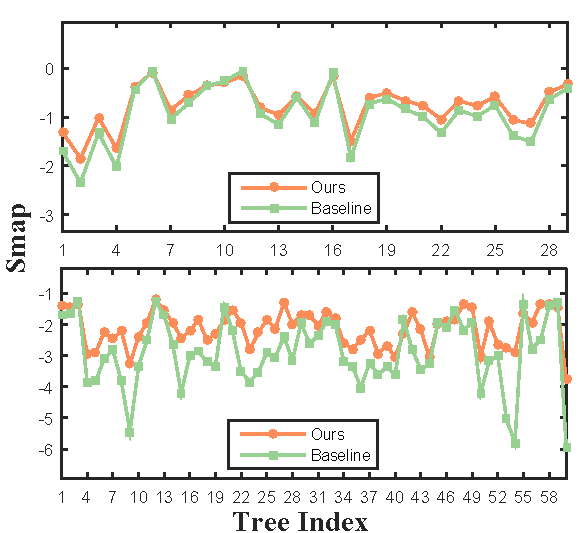
\includegraphics[width=0.7\columnwidth]{fig/v2-Smap-treeindex}
  \vspace{-1mm}
  \caption{
%  \small
  Comparison of tree mapping smoothness.}
  \vspace{-5mm}
  \label{fig:smap}
\end{figure}

\begin{figure*}[b]
	\centering
\vspace{-5mm}
    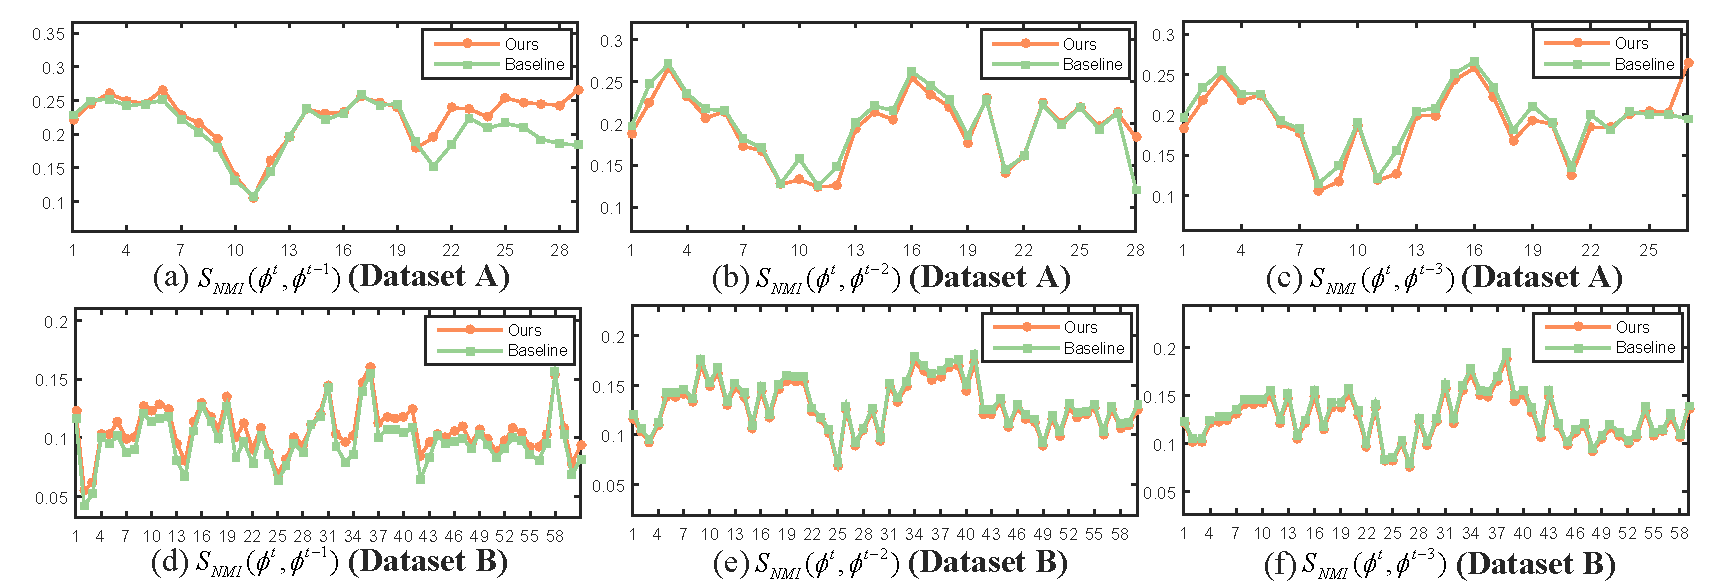
\includegraphics[width=\linewidth]{fig/v2-nmi-treeindex.pdf}
\vspace{-5mm}
	\caption{
%Comparison of NMI smoothness. x-axis represents tree index and y-axis encodes NMI smoothness.
Comparison of NMI smoothness. \kg{X}-axis represents tree index and \kg{Y}-axis encodes NMI smoothness.
}\label{fig:NMI}
\vspace{-3mm}
\end{figure*}

\begin{figure*}[b]
	\centering
    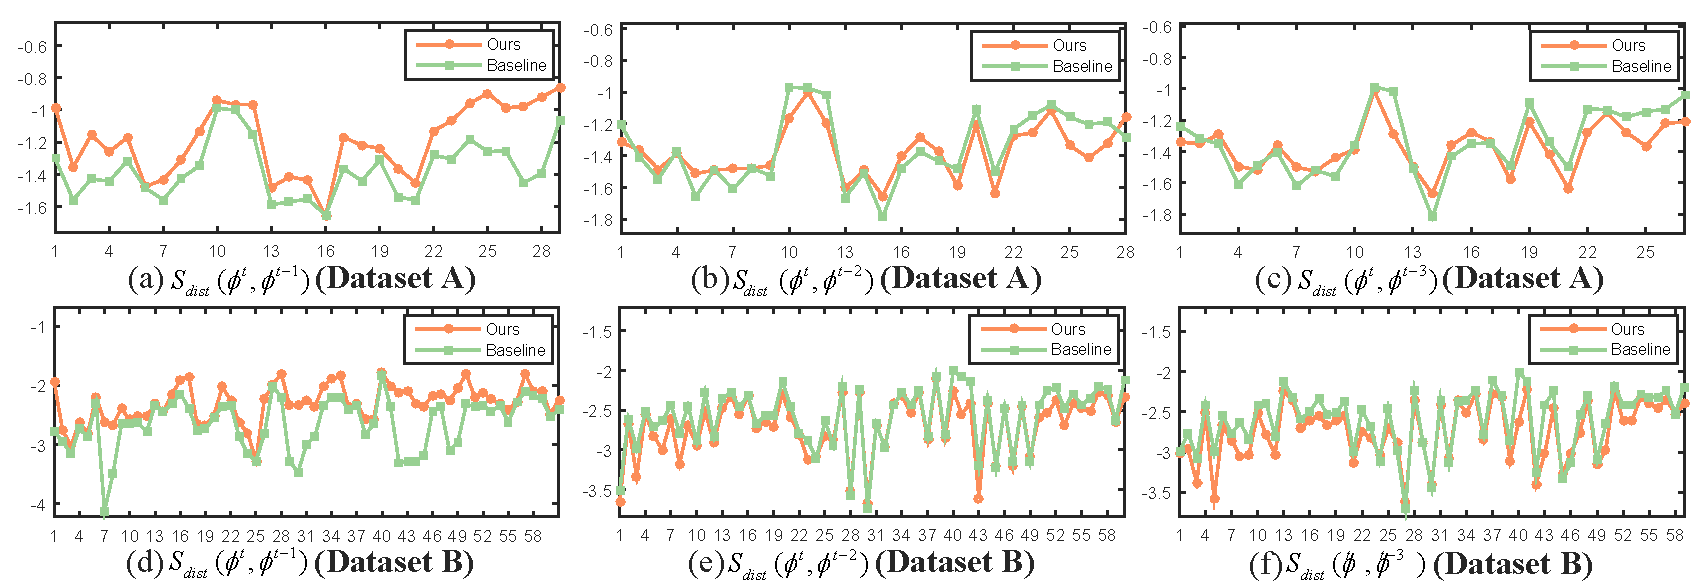
\includegraphics[width=\linewidth]{fig/v2-treedis-treeindex.pdf}
\vspace{-5mm}
	\caption{
%Comparison of tree distance smoothness. y-axis encodes tree distance smoothness.\looseness=-1
Comparison of tree distance smoothness. \kg{Y}-axis encodes tree distance smoothness.\looseness=-1
}\label{fig:distance}
%\vspace{-3mm}
\end{figure*}


%To eliminate the bias caused by the focus node selection, we randomly selected the same number of focus nodes fifty times and ran the experiments fifty times.
To eliminate bias caused by the focus node selection, the same number of focus nodes \kg{was randomly selected 50} times and the experiments \kg{were repeated 50} times.
%At each time, we computed  ${F}$ for each tree cut.
At each time, ${F}$ for each tree cut \kg{was computed}.
%Since the metric ${S_{map}}$ was defined on adjacent tree cuts, we only compute ${S_{map}}$ between adjacent tree cuts.
Since the measure ${S_{map}}$ was defined on adjacent tree cuts, we only \dc{computed} ${S_{map}}$ between adjacent tree cuts.
%\kg{Only} ${S_{map}}$ between adjacent tree cuts \kg{was computed because the metric ${S_{map}}$ was defined on adjacent tree cuts}.
%To demonstrate the global smoothness of our algorithm, ${S_{NMI}}$ and  ${S_{dist}}$ were computed between ${\phi}^t$ and each of ${\phi}^{t-1}$, ${\phi}^{t-2}$, ${\phi}^{t-3}$.
To demonstrate the global smoothness of \kg{the proposed} algorithm, ${S_{NMI}}$ and  ${S_{dist}}$, were computed between ${\phi}^t$ and each of ${\phi}^{t-1}$, ${\phi}^{t-2}$, \kg{and} ${\phi}^{t-3}$.
The results were computed by averaging the 50 trials.



\subsubsection{Results}
\label{sec:results}

%We compared the overall fitness and smoothness with the baseline.
\kg{The} overall fitness and smoothness \kg{were compared} with the baseline.
%As shown in Table~\ref{table:average}, our method can generate a much smoother structure than the baseline while maintaining a larger fitness between ${\phi}^t$ and ${\phi}^{t-1}$.
%As shown in Table~\ref{table:average}, \kg{the proposed} method can generate a much smoother structure than the baseline while maintaining a larger fitness.
As shown in Table~\ref{table:average}, \kg{the proposed} method \docpr{generates} a much smoother structure than the baseline while maintaining \docpr{greater} fitness.
% between ${\phi}^t$ and ${\phi}^{t-1}$.
%When comparing the smoothness between non adjacent tree cuts, our method is a little bit worse.
%When the smoothness between non\kg{-}adjacent tree cuts \kg{were compared}, \kg{the proposed} method \kg{performed slightly} worse\kg{,}
When the smoothness between non\kg{-}adjacent tree cuts \kg{\docpr{was} compared}, \kg{the proposed} method \kg{performed slightly} worse\kg{,}
%This is because our method only considers the adjacent tree cuts to improve the performance for streaming data.
%because \kg{the} method only \kg{considered} the adjacent tree cuts to improve the performance \kg{of data stream}.
because \kg{the} method only \kg{considered} the adjacent tree cuts to improve the performance \dc{of the data stream}.
%focus on streaming data and consider a lot about the treecuts next each other.
%Thus the global smoothness is not maintained to some extent.
Thus\kg{,} the global smoothness \kg{was} not maintained to \kg{a certain} extent.


We further compared the smoothness of our method with the baseline between trees under these measures.
%\kg{The} smoothness of \kg{the} method \kg{was further compared} with the baseline between trees under under these metrics.
%As shown in  Fig.~\ref{fig:smap}, Fig.~\ref{fig:NMI}, and Fig.~\ref{fig:distance}, the proposed streaming algorithm works as well as the baseline under the three metrics for adjacent tree cuts.
%As shown in  Fig.~\ref{fig:smap}, \ref{fig:NMI}, and \ref{fig:distance}, the proposed streaming algorithm works as well as the baseline under the three metrics for adjacent tree cuts.
As shown in  \dc{Figs}.~\ref{fig:smap}, \ref{fig:NMI}, and \ref{fig:distance}, the proposed streaming algorithm worked as well as the baseline under the three measures for adjacent tree cuts.
%For non-adjacent tree cuts, the smoothness of our algorithm is a little bit worse under the metrics ${S_{NMI}}$ and  ${S_{dist}}$.
%commonly used metrics, NMI and tree distance between trees next to each other.
%For non-adjacent tree cuts, the smoothness of \kg{the proposed} algorithm is \kg{slightly} worse under the commonly used metrics NMI and tree distance.
For non-adjacent tree cuts, the smoothness of \kg{the proposed} algorithm \dc{was} \kg{slightly} worse under the commonly used measures NMI and tree distance.
%The fitness of our algorithm at each tree was also evaluated.
The fitness of \kg{the proposed} algorithm at each tree was also evaluated.
%As shown in Fig.~\ref{fig:sf}, our algorithm is much better than the baseline at each time in all the datasets.
%As shown in Fig.~\ref{fig:sf}, \kg{the proposed} algorithm is \kg{more effective} than the baseline at each time in all the datasets.
As shown in Fig.~\ref{fig:sf}, \kg{the proposed} algorithm \dc{was} \kg{more effective} than the baseline at each time in all the datasets.
%This findings demonstrate that our algorithm can preserve the smoothness between adjacent trees as well as the fitness without sacrificing much global smoothness.
%\kg{These} findings demonstrate that \kg{the proposed} algorithm \kg{could} preserve the smoothness between \kg{the} adjacent trees as well as the fitness without sacrificing global smoothness. %\looseness=-1
\kg{These} findings demonstrate that \kg{the proposed} algorithm \docpr{can} preserve the smoothness between \kg{the} adjacent trees as well as the fitness without sacrificing global smoothness. %\looseness=-1

%We compared the overall likelihood and smoothness with the baseline.
%As shown in Table~\ref{table:average}, our method can generate a much smoother structure than the baseline while maintaining a larger likelihood.
%Besides having very good performance under the metric of $\bm{S_{map}}$, our algorithm also achieved a comparable performance under the metrics of $\bm{S_{NMI}}$ and $\bm{S_{dist}}$.
%
%
%Since the metric $\bm{S_{map}}$ is a global smoothness metric, so we further compared our method with the baseline between trees under the metrics $\bm{S_{NMI}}$ and $\bm{S_{dist}}$.
%%First, we assessed the smoothness of our evolutionary tree cut algorithm based on the three different smoothness metrics.
%As shown in Figs.~\ref{fig:NMI} and \ref{fig:distance}, the proposed evolutionary algorithm works pretty well under the commonly used metrics, NMI and tree distance.
%The fitness of our algorithm at each tree was also evaluated.
%As shown in Fig.~\ref{fig:likelihood}, the likelihood of our algorithm is as good as the baseline at each time in all the datasets.
%This findings demonstrate that our algorithm can preserve the smoothness between trees without sacrificing the likelihood of each tree.
%Finally, we demonstrated that the performance of our algorithm consistently improved with the number of focus nodes.
%From Table~\ref{table:average}, we can see that the average likelihood difference decreases with the number of focus nodes, while the average smoothness difference increases with the number of focus nodes.
%This indicates that our algorithm works better when more focus nodes are selected.

\subsection{Scalability}


\begin{figure}[t]
	%\vspace{-2mm}
	\centering
	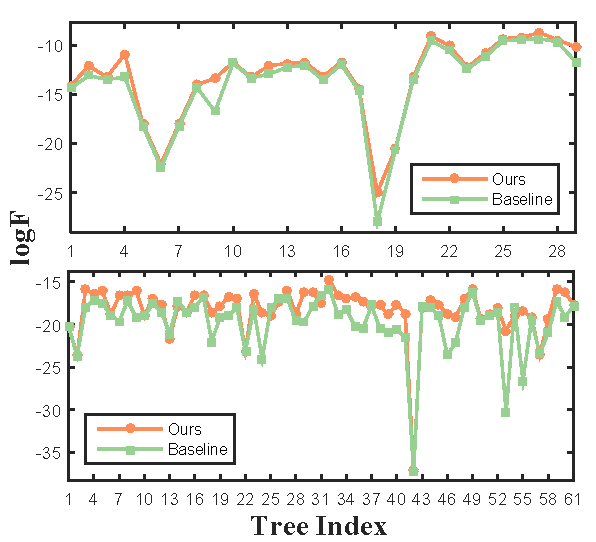
\includegraphics[width=0.7\columnwidth]{fig/v2-Sf-treeindex}
	\vspace{-1mm}
	\caption{
		%  \small
		Comparison of fitness at each tree.}
	\vspace{-6mm}
	\label{fig:sf}
\end{figure}



%In this experiment, we investigate the scalability of our algorithm.
We conducted two experiments to evaluate the scalability of our algorithm.
In the first experiment, we investigated the ability of our algorithm to handle topic trees with a large number of internal nodes ($I_{num}$).
%In the second experiment, we tested the ability of our algorithm to process long sequences of topic trees.
In the \docpr{second, we} tested the ability of our algorithm to process long sequences of topic trees.
%($P_{num}$)

%\tvcgminor{To evaluate the scalability of our algorithm, we investigate how the running time of our algorithm increases with topic tree size and number of topic trees processed.}

%\tvcgminor{\subsubsection{Criteria}}

\subsubsection{Experimental Settings}

%To assess how the running time of our algorithm increases with topic tree size, we generated
%We generated topic trees with different $I_{num}$ by copying the first ten topic trees of Dataset A different times.
%The dataset used in the first experiment was generated by copying the first ten trees in Dataset A by $s$ times ($s\in \{1,3,...,15\}$).
The dataset used in the first experiment was generated by copying the first ten trees in Dataset \docpr{A \emph{\normalsize s}} times ($s\in \{1,3,...,15\}$).
%To generate topic trees with different $I_{num}$, we copied the first ten trees generated using Dataset A by $s$ times ($s\in \{1,3,...,15\}$). %resulting in topic trees with an average $I_{num}$ of $\{118, 354, ..., 1770\}$.
As a result, we obtained eight groups of topic trees with varied $I_{num}$ ($I_{num}\in\{118, 354, ..., 1770\}$). % with the average $I_{num}$ per tree range from 118 to 1770. %of each set range from 118 to 1770. %$\{118, 354, ..., 1770\}$ internal nodes for each tree on average. % internal nodes on average.
For each group of topic trees, we treated the first five trees as old trees and evaluated the average time to process the 6th to 10th trees. %last five topic trees. %the
In our experiments, focus nodes were randomly selected to avoid any biased conditions.
To eliminate randomness caused by the focus node selection, we randomly selected the given number $m$ ($m\in\{1,3,5\}$) of focus nodes 50 times and ran the experiment 50 times.
Results were computed by averaging the 50 trials.

%we randomly selected 50 sets of focus nodes for the same number of focus nodes $m$ ($m\in\{1,3,5\}$).
%The results were calculated by averaging the 50 trials.
%we evaluated the running time under different numbers of focus nodes ($m\in\{1,3,5\}$) and randomly selected 50 sets of focus nodes for each $m$.



In the second experiment, we used the 30 topic trees in Dataset A.
%To assess how the running time of our algorithm increases with $P_{num}$, the 30 topic trees of Dataset A were used.
Specifically, we regarded the first $P_{num}$ ($P_{num}\in \{7,9,...29\}$) trees as old trees, and evaluated the time to process the $(P_{num}+1)$-th tree.
%To eliminate the bias caused by the number of internal nodes in the $(P_{num}+1)$th tree, we normalized the running time by multiplying it with $I_{max}/I_{cur}$
%Other settings are same as the first experiment.
\docpr{All other settings were the} same as the first experiment.
%Similar to the first experiment, we randomly selected 50 sets of focus nodes for each $m\in\{1,3,5\}$ and calculated the results by averaging the 50 trials.\looseness=-1 %repeated the experiments 50 times.



The experiments were run on a workstation with an Intel Xeon E5-2630 CPU (2.4 GHz) and 64GB Memory.


\subsubsection{Results}

As shown in Fig.~\ref{fig:exp-time-Inum}, the running time of our algorithm increases at an approximate quadratic rate with the increase of $I_{num}$.
%our algorithm is able to deal with large topic trees.
%scale well with $I_{num}$.
%For $m=5$, our algorithm can process topic trees with 1770 internal nodes in 66 seconds.
For $m=5$, our algorithm can process topic trees with \docpr{1,770} internal nodes in 66 seconds.
This demonstrates that our algorithm can handle large topic trees.
% shows how the running time increases with $I_{num}$ under different $m$.


%Next, we demonstrate the scalability of our algorithm in regards to $P_{num}$ under different $m$.
Next, we \docpr{demonstrated} the scalability of our algorithm in regards to $P_{num}$ under different \emph{\normalsize m}.
%Here we used normalized running time to eliminate bias caused by different sizes of the topic trees.
\docpr{We} used \docpr{a} normalized running time to eliminate \docpr{any} bias caused by different sizes of the topic trees.
Normalized running time is calculated by multiplying real running time with $(I_{avg}/I_{cur})^2$.
%Here $I_{avg}$ is computing by averaging $I_{num}$ of all trees and $I_{cur}$ is $I_{num}$ of the $(P_{num}+1)$-th topic tree.
Here $I_{avg}$ is \docpr{computed} by averaging $I_{num}$ of all trees and $I_{cur}$ is $I_{num}$ of the $(P_{num}+1)$-th topic tree.
As shown in Fig.~\ref{fig:exp-time-Pnum}, the normalized running time increases slowly with the increase of $P_{num}$ and the results are consistent across different $m$.
This indicates that our algorithm can process long sequences of topic trees efficiently.\looseness=-1

\begin{figure}[t]
%\vspace{-2mm}
\centering
{
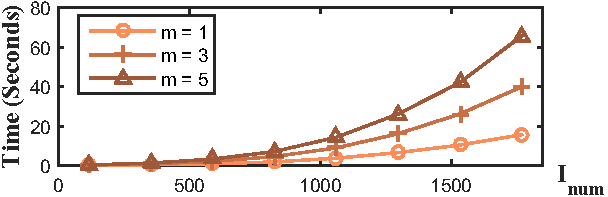
\includegraphics[width=0.36\textwidth]{fig/TotalTime-TopicNumber.pdf}
}
\caption{Running time vs. number of internal nodes in the topic tree ($I_{num}$) vs. number of focus nodes ($m$).}
\label{fig:exp-time-Inum}
\vspace{-1mm}
\end{figure}


\begin{figure}[t]
%\vspace{-2mm}
\centering
{
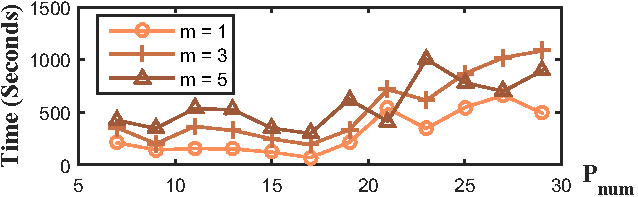
\includegraphics[width=0.36\textwidth]{fig/TotalTime-TreeCount.pdf}
}
\caption{Normalized running time vs. number of topic trees processed ($P_{num}$) vs. number of focus nodes ($m$).}
\label{fig:exp-time-Pnum}
\vspace{-5mm}
\end{figure}


\section{Case Study}
%This section highlights how the system helps analyze large text streams by applying it to the news dataset \emph{B} (Section~\ref{sec:results}).
%This section highlights the system \kg{analysis of} large text streams \kg{applied} to the news dataset \emph{B} (Section~\ref{sec:results}).
%\kg{In this section, we demonstrate the usage scenarios of our approach in real-world news/Twitter datasets.}
In this section, we demonstrate the usage scenarios of our approach \dc{using} real-world datasets.


%, Obama data.
%444,432 news articles that contain the keyword ``Obama,'' were collected from Sep. 1, 2012 to Jan. 14, 2013.
%Grouped by week, the articles were organized into 18 topic trees. %(Fig.~\ref{fig:obamatree}).
%%The average number of the first level nodes is 41, and the tree depth is 5($\pm 1$).
%The tree depths varied from 4 to 5, the total node numbers changed from 144 to 297, and the node
%number of the first level ranged from 18 to 79.
%\begin{figure}[ht]
%  \centering
%  \includegraphics[width=\columnwidth]{fig/obamatree}
%  \caption{Example topic tree for Obama data.}
%  \label{fig:obamatree}
%\end{figure}
\begin{figure*}[t]
\centering
%\vspace{-3mm}
\centering
  \includegraphics[width=\linewidth]{fig/Teaser}
    \vspace{-3mm}
  \caption{
%  \small
  %Overview of streaming hierarchical topics .
  %It provides an
%  Comparative analysis between the severity of epidemic and the intensity of public opinion in the Ebola dataset.
  Comparative analysis between the severity of \dc{the} epidemic and the intensity of public opinion in the Ebola dataset.
  %(a) Before Sep. 27, the most severe region, Africa, is the key focus of the public opinion.
  (a)  \kg{The region with the most severe cases (i.e., Africa)} was the key focus of public opinion \kg{before Sep. 27, 2014}.
  %During this period, the severity of epidemic is consistent with the intensity of public opinion.
  \kg{Epidemic severity during this period} was consistent with \kg{public opinion intensity.}
  %(b) After Sep. 27, there is an explosive growth of public discussion on the non-Africa regions.
  %(b) An explosive growth of public discussion on non-African regions \kg{occurred after Sep. 27.}
  (b) An explosive growth of public discussion \docpr{in} non-African regions \kg{occurred after Sep. 27.}
  %During this period, the intensity of public opinion is different with the severity of epidemic.
  \kg{Public opinion intensity during this period was inconsistent with epidemic severity.}
  }
%\vspace{-4mm}
\label{fig:msoverview}
\vspace{-5mm}
\end{figure*}
\subsection{Ebola Data}

%Ebola is a disease of humans and other primates caused by ebolaviruses.
%The largest outbreak of Ebola is the ongoing epidemic in West Africa.
%By Mar. 31, 2015, this outbreak has 25,263 reported cases resulting in 10,477 deaths.
%\kg{As of} Mar. 31, 2015, this outbreak \kg{had} 25,263 reported cases \kg{that resulted} in 10,477 deaths.
%We conducted the case study with a professor (P2) majored in public opinion analysis on healthcare.
%\kg{The} case study \kg{was conducted} with a professor (P2) \kg{who} majored in public opinion analysis on healthcare.
\kg{The} case study \kg{was conducted} with a professor (P2) \kg{who} majored in public opinion analysis \dc{in} healthcare.
%This case study aims at illustrating how TopicStream helps the expert examine the relationship between the severity of epidemic and the intensity of public opinion.
%This case study aims \kg{to illustrate} how TopicStream helps the expert examine the relationship between the severity of \kg{an} epidemic and the intensity of public opinion.
In this case study, we illustrate how TopicStream helps an expert examine the relationship between the severity of an epidemic (e.g., Ebola) and the intensity of public opinion.
%The severity of epidemic is measured by the reported case and death counts.
%The severity of \kg{the} epidemic is measured by the reported \kg{number of cases} and \kg{deaths}.
The severity of \kg{the} epidemic \docpr{was} measured by the reported \kg{number of cases} and \kg{deaths}.
%The intensity of public opinion is represented by the number of news articles and tweets at that time step (the width of the topic stripe).
The intensity of public opinion \docpr{was} represented by the number of news articles and tweets at that time step (the width of the topic stripe).
A wider stripe indicated more intense public opinion (Fig.~\ref{fig:msoverview}).\looseness=-1
%\kg{Fig.~\ref{fig:msoverview} shows that a} wider stripe \kg{indicated the intenser} public opinion.
%Moreover, it also demonstrates the capability of our tool in facilitating the expert to discover the major causes and the government's guidance on the opinion development.
%Moreover, it also demonstrates the \kg{ability} of our tool \kg{to enable} the expert to discover the major causes \kg{of} and the \kg{government} guidance on opinion development.

%A dataset that contains both news articles and tweets is used, which is collected by using keyword ``Ebola.''
%A dataset that contains both news articles and tweets collected by using keyword ``Ebola'' \kg{was used} (Dataset A).
A dataset that contains both news articles and tweets collected by using \docpr{the} keyword ``Ebola'' \kg{was used} (Dataset A).
Table~\ref{table:ebola} shows the statistics of the dataset.
\begin{table}[h]

\vspace{-3mm}
    \vspace{1mm}

    \centering
    \scalebox{0.8}{

    \begin{tabular}{|c|c|c|c|c|c|}

    \hline
    %Data & Time span & N\_num & T\_num & Depth & I\_num \\
    Data & Time span & $N_{num}$ & $T_{num}$ & \xiting{$h$} & $I_{num}$ \\
    \hline
   \emph{Old} & 7/27/2014-9/27/2014 & 51,318 & 7,161 & 3-4 & 77-150\\
   \hline
    \emph{New} & 9/28/2014-2/21/2015 & 156,088 & 15,558,371 & 3-5 & 34-223\\
   \hline
    \end{tabular}
    }
%        \vspace{-2mm}
    \caption{
%    \small
%The statistics of the Ebola dataset.
\kg{Statistics} of the Ebola dataset. \xiting{Here $N_{num}$ denotes the number of news articles, $T_{num}$ represents the number of tweets, $h$ is the tree depth, and $I_{num}$ denotes the number of internal nodes in the tree.}
}
\vspace{-5mm}
    \label{table:ebola}
\end{table}



\noindent \textbf{\normalsize Spread of Ebola outbreak.}
We first provided the professor (P2) with an overview of the old Ebola data.
%\kg{P2 was first provided} with an overview of the old Ebola data.
%The old data (before Sep. 27, 2014) is shown in Fig.~\ref{fig:msoverview}(a).
The old data (before Sep. 27, 2014) is shown in Fig.~\ref{fig:msoverview}(a).
%The news articles from Sep. 28 to Oct. 4 come in a streaming way Fig.~\ref{fig:msoverview}(b).
The news articles from Sep. 28 to Oct. 4 \kg{appeared in a streaming manner, as shown in} Fig.~\ref{fig:msoverview}(b).
%Based on topic keywords and corresponding news articles in Fig.~\ref{fig:msoverview}(a), the professor immediately identified the major topics in the news stream.
\kg{Using} topic keywords and corresponding news articles in Fig.~\ref{fig:msoverview}(a), %\kg{P2} immediately identified the major topics in the news stream, which are encoded by blue, pink, and yellow colors.
\kg{P2} immediately identified the major topics in the news stream, which \docpr{were} encoded \docpr{as} blue, pink, and \docpr{yellow.}
As in~\cite{cui2014}, we used the mean-shift clustering algorithm to cluster the topic at the first level since it is the most abstract level and can represent the topic tree very well.
For each cluster, we chose the topic closest to the cluster center as one focus topic.
%In this dataset, three focus topics encoded by blue, pink, and yellow colors, are automatically extracted by this method.
%, including ``Ebola-infected aid workers'' (blue), ``Ebola outbreak in Africa'' (pink), and ``Ebola patients and suspects outside Africa'' (yellow).


%By examining the incoming news articles on the pink topic stripe, ``Ebola outbreak in Africa'' (Fig.~\ref{fig:msoverview}A), she found that the epidemic is very serious in Africa.
By examining the incoming news articles on the pink topic stripe, ``Ebola outbreak in Africa'' (Fig.~\ref{fig:msoverview}A), \kg{P2} found that the epidemic \kg{was extremely} serious in Africa.
%It not only has the high death number (``Ebola: Killer virus death toll passes 3,000,'' Fig.~\ref{fig:msoverview}A1), but also the rapid growth of infections.
%It not only has the high death number (``Ebola: Killer virus death toll passes 3,000,'' Fig.~\ref{fig:msoverview}A1), but also the rapid growth of infections.
%\kg{The epidemic caused a large number of deaths} (``Ebola: Killer virus death toll passes 3,000,'' Fig.~\ref{fig:msoverview}A1) \kg{and the} growth of infections \kg{was rapid}.
\kg{The epidemic caused a large number of deaths} (Fig.~\ref{fig:msoverview}A1) \kg{and the} \dc{spread} of infections \kg{was rapid}.
%For example, in the news article ``Ebola could hit up to 1.4 mln West Africans by January: U.S. CDC,'' it is said ``Reported cases in Liberia are doubling every 15 to 20 days, and those in Sierra Leone are doubling every 30 to 40 days'' (Fig.~\ref{fig:msoverview}A2).
%For example, news article ``CDC worst case scenario for Ebola: 1.4 million cases'' mentioned that reported cases in Liberia are doubling every 15 to 20 days and those in Sierra Leone are doubling every 30 to 40 days (Fig.~\ref{fig:msoverview}A2).
For example, \docpr{the} news article \docpr{entitled} ``CDC worst case scenario for Ebola: 1.4 million cases'' mentioned that reported cases in Liberia \docpr{were} doubling every 15 to 20 days and those in Sierra Leone \docpr{were} doubling every 30 to 40 days (Fig.~\ref{fig:msoverview}A2).
%The blue topic stripe containing keywords ``dr,'' ``sacra,'' etc. talks about ``Ebola-infected aid workers''.
The blue topic stripe \kg{contains} keywords ``dr,'' ``sacra,'' \kg{and} talks about ``Ebola-infected aid workers.''
%``sacra'' is the last name of one of the aid workers, Dr. Rick Sacra.
\kg{``Sacra''} is the last name of \kg{Dr. Rick Sacra}, one of the aid workers.
%By examining the news articles in the archive area (Fig.~\ref{fig:msoverview}B), professor P2 learned that there are two aid workers returned to the U.S. for the treatment (``Second American health worker with Ebola arrives in U.S.'').
By examining the news articles in the archive area (Fig.~\ref{fig:msoverview}B), \kg{P2} learned that two aid workers returned to the U.S. for \kg{treatment}.
% (``Second American health worker with Ebola arrives in U.S.'').
%The increased width in the stack area (Fig.~\ref{fig:msoverview}C) talked about their recovery (``2 American Ebola patients released from hospital'').
The increased width in the stack area (Fig.~\ref{fig:msoverview}C) \kg{discussed} their recovery.
% (``2 American Ebola patients released from hospital'').
%Fig.~\ref{fig:msoverview}D and Fig.~\ref{fig:msoverview}E in the river area are about the third and fourth infected aid workers.
%Figs.~\ref{fig:msoverview}D and \kg{\ref{fig:msoverview}E} in the river area are about the third and fourth infected aid workers.
Figs.~\ref{fig:msoverview}D and \kg{\ref{fig:msoverview}E} in the river area are \dc{related to} the third and fourth infected aid workers.
%From the above exploration, she concluded that there are several infected aid workers, however, the situation is not serious.
From the \kg{preceding} exploration, \kg{P2} concluded that several aid workers \kg{had been infected;} however, the situation \kg{was} not serious.
%From the word cloud ( Fig.~\ref{fig:msoverview}F ) of the yellow topic stripe, professor P2 observed keywords like ``suspected,'' ``tested,'' ``york,'' ``sinai'' etc.
%From the word cloud ( Fig.~\ref{fig:msoverview}F ) of the yellow topic stripe, \kg{P2} observed keywords \kg{such as} ``suspected,'' ``tested,'' ``york,'' ``sinai.''
%From the word cloud ( Fig.~\ref{fig:msoverview}F ) of the yellow topic stripe, \kg{P2} observed keywords \kg{such as} ``suspected,'' ``york,'' \dc{and} ``sinai.''
From keywords ``suspected,'' ``york,'' \dc{and} ``sinai'' in the word cloud of the yellow topic stripe (Fig.~\ref{fig:msoverview}F)),  
%She found this topic is about ``Ebola patients and suspects outside Africa.''
\kg{P2} concluded \kg{that} this topic \kg{was} about ``Ebola patients and suspects outside Africa.''
%After reading the corresponding news articles before before Sep. 27, she concluded that there are only several suspects outside Africa and the situation is not serious.
After reading the corresponding news articles before Sep. 27, \kg{P2} concluded that only \kg{a few} suspects \kg{were} outside Africa and the situation \kg{was} not serious.\looseness=-1

\begin{figure*}[t]
	\centering
	\vspace{-2mm}
	\centering
	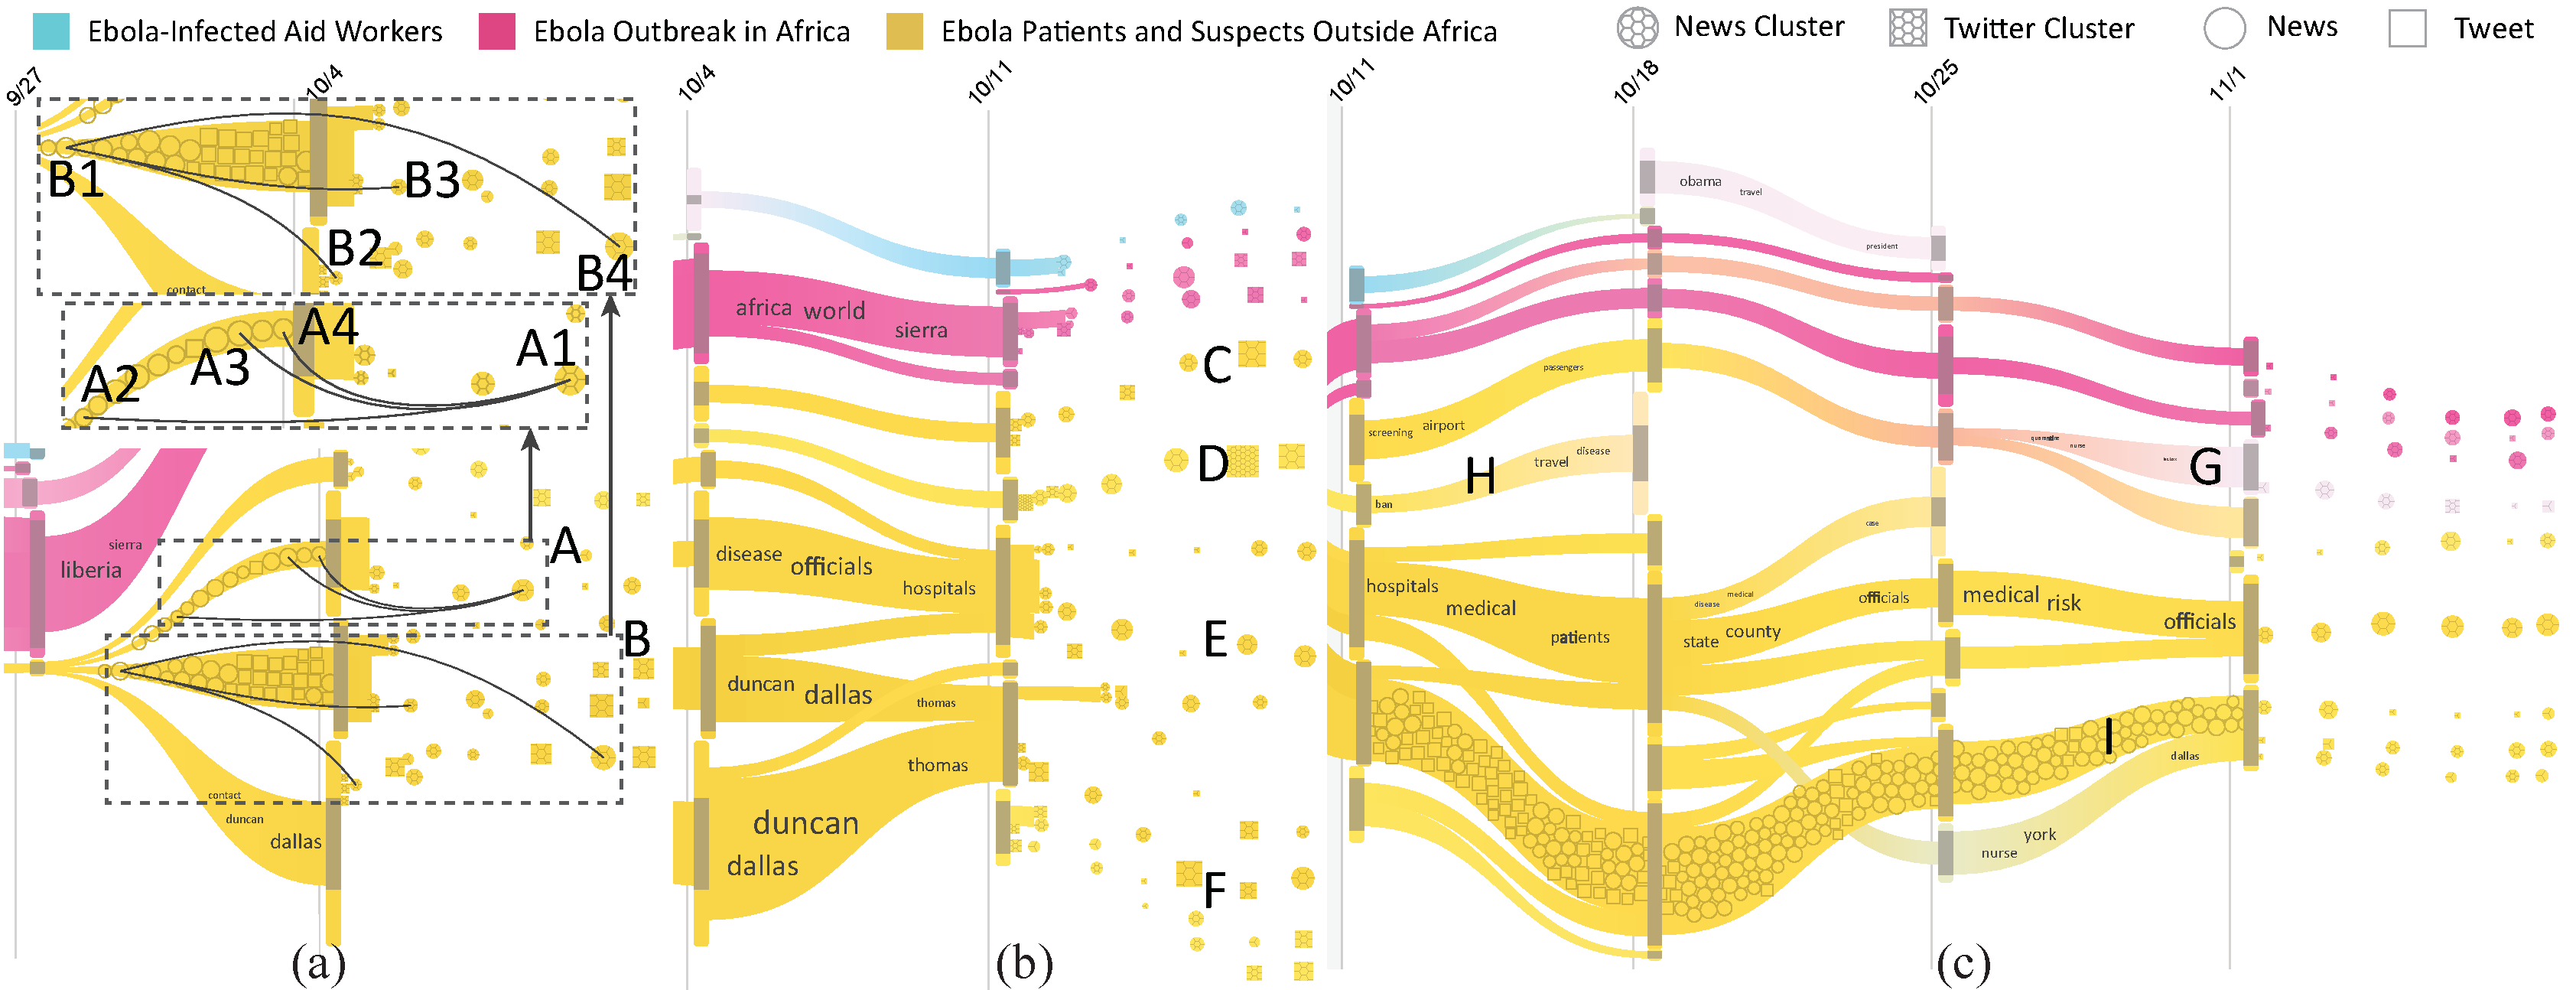
\includegraphics[width=\linewidth]{fig/ebola}
	\vspace{-3mm}
	\caption{
		%  \small
		%Explosive discussion on the the reported case outside Africa: (a) Oct. 5-11; (b) Oct. 12-18; (c) Nov. 2-8.
		%Explosive discussion on reported \kg{cases} outside Africa: (a) Oct. 5 to 11; (b) Oct. 12 to 18; (c) Nov. 2 to 8.
		Explosive discussion \docpr{of} reported \kg{cases} outside Africa: (a) Oct. 5 to 11; (b) Oct. 12 to 18; (c) Nov. 2 to 8.
	}
	\vspace{-5mm}
	\label{fig:ebola}
\end{figure*}

\noindent \textbf{\normalsize Explosive discussion on Ebola outside Africa.}
%Professor P2 found that the severity of epidemic is consistent with the intensity of public opinion before Sep. 27 (Fig.~\ref{fig:msoverview}(a)).
\kg{P2} found that the severity of \kg{the} epidemic \kg{was} consistent with the intensity of public opinion before Sep. 27 (Fig.~\ref{fig:msoverview}(a))\kg{,}
%Namely, the wider the stripe, the more intense the public opinion.
that is, the stripe \kg{was wider}, \kg{which indicated} more intense public opinion.
%However, after Sep. 28, there is an explosive discussion on Ebola outside Africa (Fig.~\ref{fig:msoverview}(b)).
However, as indicated by the increasing number of yellow circles and squares in the visualization (Fig.~\ref{fig:msoverview}(b)), there is an explosive discussion on Ebola outside Africa \kg{occurred} after Sep. 27.
%Professor P2 was curious about such a change, so she continued to explore the incoming data.
P2 was curious about such a change\kg{;} \kg{thus, the exploration of} the incoming data \kg{continued}.


%She noticed that the explosion began at the news cluster denoted by Fig.~\ref{fig:msoverview}G, which contains many news articles.
She noticed that the explosion began at the news cluster denoted by Fig.~\ref{fig:msoverview}G, which \kg{contained} many news articles.
The news cluster was then followed by several Twitter clusters.
%After some exploration, she found the news cluster is mainly about the first case of Ebola in the US (``CDC confirms first case of Ebola in US'').
After some exploration, \kg{P2} found \kg{that} the news cluster \kg{was} mainly about the first case of Ebola in the US.
 %(``CDC confirms first case of Ebola in US'').
%The patient, Thomas Duncan, had come into contact with as many as 80 people.
The patient, Thomas Duncan, had \kg{been exposed to} as many as 80 people.
%The first confirmation case led to a lot of discussion on Twitter (``....hmm Fwd: US Government Confirms an Ebola Case in Texas! http://t.co\/GNcFZGWzEz sponsor=femiolulana'') and created fears (``I don't even know what're symptoms are for Ebola But I think I got them'').
The first confirmed case led to \kg{numerous} discussion\kg{s} on Twitter
 %(``....hmm Fwd: US Government Confirms an Ebola Case in Texas! http://t.co\/GNcFZGWzEz sponsor=femiolulana'')
and created fear.
% (``I don't even know what're symptoms are for Ebola But I think I got them'').
%Because of the heightened attention from the public and media, this topic is divided into four sub-topics:
Because of the heightened attention from the public and media, this topic \docpr{was} divided into four sub-topics:
1) the further report of suspects (Fig.~\ref{fig:msoverview}H);
2) government actions (Fig.~\ref{fig:msoverview}I);
3) treatment of the patient (Fig.~\ref{fig:msoverview}J);
%and 4) search for people who had some form of contact with the patient (Fig.~\ref{fig:msoverview}K).
and 4) \docpr{the} search for people who had some form of contact with the patient (Fig.~\ref{fig:msoverview}K).\looseness=-1
%\kg{This} topic is divided into four sub-topics \kg{because of the heightened attention from the public and media.}
%\kg{The Topics are} 1) further report of suspects (Fig.~\ref{fig:msoverview}H); 2) \kg{government} actions (Fig.~\ref{fig:msoverview}I); 3) \kg{treatment} of the patient (Fig.~\ref{fig:msoverview}J); and 4) search \kg{for} people who \kg{had some form of} contact with the patient (Fig.~\ref{fig:msoverview}K).

%Professor P2 commented that the public and news media in the US did not pay too much attention to the Ebola epidemic when it happened in Africa (before Sep. 27) and observed it in the other's perspective.
%\kg{P2} commented that the public and news media in the US \kg{paid minimal} attention to the Ebola epidemic happened in Africa \kg{before Sep. 27, observing the epidemic from the other's perspective.}
%\kg{P2} commented that the public and news media in the US \kg{paid minimal} attention to the Ebola epidemic \dc{in} Africa \kg{before Sep. 27, observing the epidemic from the other's perspective.}
\kg{P2} commented that the public in the US \kg{paid minimal} attention to the Ebola epidemic \dc{in} Africa \kg{before Sep. 27, observing the epidemic from the other's perspective.}
This is consistent with the theory of alterity (otherness)~\cite{otherness}.
%consistent with the theory of alterity (otherness)~\cite{otherness}.
%It broke such a perspective when it happened around themselves and led to an intensive discussions on news media and Twitter.
%\kg{When the epidemic} happened \kg{in the US, the perspective changed} and led to intensive discussions on news media and Twitter.
\kg{When the epidemic} \dc{arrived} \kg{in the US, the perspective changed} and led to \dc{intense} discussions on news media and Twitter.
%She further explained the spread of the first case in the US also disclosed another phenomenon.
\kg{P2} further explained \kg{that} the spread of the first case in the US also disclosed another phenomenon.
%Since the news media reported the first case wantonly, the severity of the epidemic was overestimated and fears were created among average persons.
%Since the news media reported the first case wantonly, the severity of the epidemic was overestimated and fears were created among average \dc{people}.
Since the news media reported the first case wantonly, the severity of the epidemic was overestimated and \docpr{fear was} created among average \dc{people}.
%\kg{The} severity of the epidemic \kg{was} \kg{overestimated} and fears were created among average persons \kg{because the news media reported the first case wantonly and because}
%This is due to that the human perceptual world is often influenced by the pseudo society built by the media.
This is \dc{because human perception} is often influenced by the pseudo society built by the media.
%the \kg{human} perceptual world is often influenced by the pseudo society built by the media.
%Under such situation, it is very important for the government to take actions to guide the public opinion.
Under such \kg{a} situation, the government \kg{must} guide public opinion.

%\noindent \textbf{Government's action and guidance.}
\noindent \textbf{\normalsize \kg{Action} and guidance \kg{of the government}.}
%Professor P2 wanted to know the US government's actions on the epidemic.
%Thus she continued examining more new documents.
%\kg{P2} continued examining new documents \kg{to know the actions of the US government on the epidemic}.
\kg{P2} continued examining new documents to \dc{learn} the actions of the government \dc{regarding} the epidemic.
%She found there was few discussion on Twitter on topic ``government's actions'' from Oct. 5 to Oct. 11 (Fig.~\ref{fig:ebola}A).
%She found few discussion on Twitter on topic ``\dc{government actions}'' from Oct. 5 to Oct. 11 (Fig.~\ref{fig:ebola}A)\kg{,}
%She found few \dc{discussions} on Twitter on topic ``\dc{government actions}'' from Oct. 5 to Oct. 11 (Fig.~\ref{fig:ebola}A)\kg{,}
She found few \dc{discussions} on Twitter on \docpr{the} topic ``\dc{government actions}'' from Oct. 5 to Oct. 11 (Fig.~\ref{fig:ebola}A)\kg{,}
%This indicates that this topic does not attract too much attention from the public.
\kg{indicating} that this topic \kg{failed to} attract \kg{public} attention.
%On the contrary, there was a lot of discussion on Twitter on the death of the Ebola patient (Fig.~\ref{fig:ebola}B).
On the contrary, \kg{numerous discussions} on Twitter \kg{focused} on the death of \kg{an} Ebola patient (Fig.~\ref{fig:ebola}B).\looseness=-1


%In order to figure out the reason, she examined these two topics in Fig.~\ref{fig:ebola}(a) and found one representative cluster (A1, ``CDC urges hospitals to follow Ebola-related protocols'') and document (B1, ``Dallas hospital isolating patient being tested for Ebola'').
\kg{To identify} the reason, \kg{P2} examined these two topics in Fig.~\ref{fig:ebola}(a) and found one representative cluster (Fig.~\ref{fig:ebola}A1, ``EbolaCDC urges hospitals to follow Ebola-related protocols'') and document (Fig.~\ref{fig:ebola}B1, ``Dallas hospital isolating patient being tested for Ebola'').
%She then explored their similar documents/clusters in the adjacent time points to know how the topics evolved in the stream.
%She then explored similar documents \kg{or} clusters in the adjacent time points to know \kg{the evolution of} the topics in the stream.
She then explored similar documents \kg{or} clusters in the adjacent time steps to \dc{determine} \kg{the evolution of} the topics in the stream.
%From the links and corresponding documents in Fig.~\ref{fig:ebola}A, she found the government immediately took actions and prepared for Ebola before Oct. 1: 1) Sep. 30, ``Health Ministry to distribute 10,000 PPEs on Thursday'' (A2); 2) Oct. 2, ``Local hospitals prepared in case of Ebola'' (A3); 3) Oct. 2, ``Ebola 'unlikely' but South prepared'' (A4).
From the links and corresponding documents in Fig.~\ref{fig:ebola}A, \kg{P2} found \kg{that} the government immediately took \kg{action} and prepared for Ebola before Oct. \kg{4}, \kg{as shown by the following news articles}: 1) Sep. 30, ``Health Ministry to distribute 10,000 PPEs on Thursday'' (Fig.~\ref{fig:ebola}A2); 2) Oct. 2, ``Local hospitals prepared in case of Ebola'' (Fig.~\ref{fig:ebola}A3); \kg{and} 3) Oct. 2, ``Ebola `unlikely' but South prepared'' (Fig.~\ref{fig:ebola}A4).
%From the links and corresponding clusters, the professor got the idea that the patient's condition was getting worse and finally died: 1) Oct. 5, ``Dallas Ebola patient is in critical condition, hospital say'' (B2); 2) Oct. 5, ``Ebola patient in Dallas 'took a turn for the worse'' (B3); 3) Oct. 8, ``Dallas Ebola Patient Dies'' (B4).
From the links and corresponding clusters in Fig.~\ref{fig:ebola}B, \kg{P2 realized} that the patient's condition \kg{worsened and led to death, as indicated by the following news articles}: 1) Oct. 5, ``Dallas Ebola patient is in critical condition, hospital says'' (Fig.~\ref{fig:ebola}B2); 2) Oct. 5, ``Ebola patient in Dallas takes a turn for worse'' (Fig.~\ref{fig:ebola}B3); \kg{and} 3) Oct. 8, ``Dallas Ebola Patient Dies'' (Fig.~\ref{fig:ebola}B4).
%The professor believed that the government took the right action in time.
\kg{P2} believed that the government acted promptly.
However, the death of the patient
%The key leading to the uncontrolled public opinion is the death of the patient.
\kg{led} to uncontrolled public opinion.

\begin{figure*}[t]
	\centering
	%\vspace{-3mm}
	\centering
	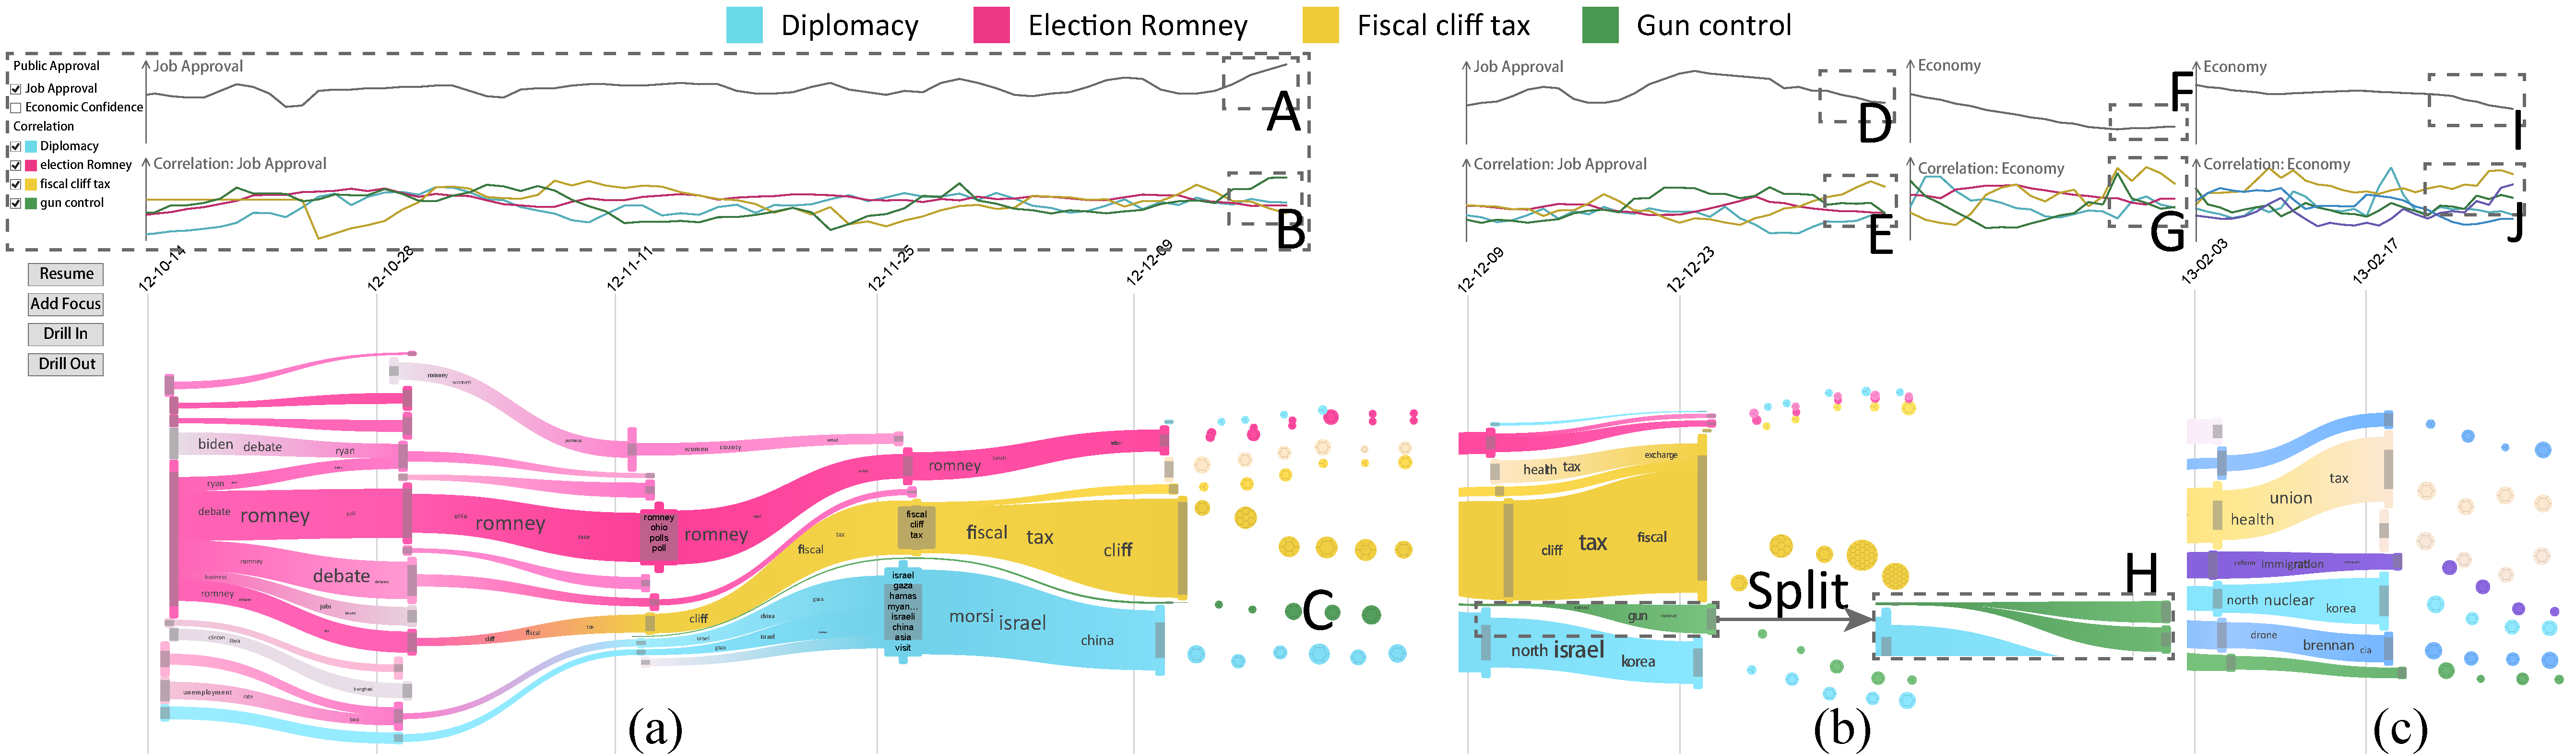
\includegraphics[width=\linewidth]{fig/obamacase1}
	\vspace{-4mm}
	\caption{
		Significant changes in public opinion in the Obama dataset.
		%Correlations are shown to help analyzing the reason for the changes.
		%(a) Presidential approval rate affected by topic ``Gun Control.''
		(a) Presidential approval \docpr{rating} affected by topic ``Gun Control.''
		%   The topic ``gun control'' (green) was triggered by a shooting accident.
		%   %Topic ``Gun Control'' (green) had a boost in the period of Obama's second term of office.
		%   Obama's response for this accident fit public opinion. This may be one leading factor of the increase of his job approval.
		%(b) A decrease of presidential approval and economic confidence caused by the fiscal cliff crisis.
		(b) A decrease \kg{in} presidential approval and economic confidence caused by the fiscal cliff crisis.
		%Public attention transited to topic ``Fiscal Cliff.”
		%Public attention transferred to ``fiscal cliff". Obama's mistakes in handling the crisis caused critics to him and the crisis led to low economic confidence.
		%(c) Another low economic confidence caused by failed negotiation on spending cuts of the government.
		%(c) Another low economic confidence \kg{rating} caused by failed negotiation\kg{s} on spending cuts of the government.
		(c) Another low economic confidence \kg{rating} caused by failed negotiation\kg{s} on \docpr{government spending cuts}.
		%Initial layout of media topics related to ``Obama", public approval line and their correlation. Topics with high correlation or topic transition caused change in public approval.
		%High correlation between the yellow topic and the economic approval and Obama's failure on handling the economic crisis caused the .
	}
	\vspace{-5mm}
	\label{fig:obamacase1}
\end{figure*}


%Next, the documents in the week of Oct. 11 streamed in.
\kg{The} documents \kg{that subsequently streamed in were from} the week of Oct. 11.
%As shown in Fig.~\ref{fig:ebola}(b), public attention on topic ``government's action'' kept on decreasing (E).
%As shown in Fig.~\ref{fig:ebola}(b), public attention on  topic ``\dc{government action}'' \kg{decreased} (Fig.~\ref{fig:ebola}E)\kg{, whereas}
As shown in Fig.~\ref{fig:ebola}(b), public attention \docpr{to the}  topic ``\dc{government action}'' \kg{decreased} (Fig.~\ref{fig:ebola}E)\kg{, whereas}
%While there is increasing discussions on Twitter on topics ``airport screening'' (C, ``Ebola Screenings Begin at US Airports''), ``travel ban'' (D, ``RT @CronkiteSays: VIEWER POLL\#N\#Do you support a travel ban from Ebola inflicted countries?''), and ``infected nurse'' (F, ``Dallas Nurse With Ebola Identified'').
discussions on Twitter on topics ``airport screening'' (Fig.~\ref{fig:ebola}C, ``Ebola Screenings Begin at US Airports''), ``travel ban'' (Fig.~\ref{fig:ebola}D, ``RT @CronkiteSays: VIEWER POLL\#N\#Do you support a travel ban from Ebola inflicted countries?''), and ``infected nurse'' (Fig.~\ref{fig:ebola}F, ``Dallas Nurse With Ebola Identified'') \kg{increased}.
%The public pay further attention to negative messages.
%The public \kg{paid} further attention to negative messages.
The public \kg{paid} \dc{more} attention to negative messages.
%The situation was improved after three weeks (Fig.~\ref{fig:ebola}(c)).
The situation \dc{improved} after three weeks (Fig.~\ref{fig:ebola}(c)).
%The professor analyzed the documents and concluded three reasons for this change.
\kg{P2} analyzed the documents and \kg{specified} three reasons for this change.
%First, the evolvement of ``airport screening'' into another new topic shifted the public attention (F).
%First, the \kg{change} of ``airport screening'' into another new topic shifted the public attention (\kg{G}).
First, the \kg{change} \dc{from topic} ``airport screening'' \dc{to} another \dc{topic} shifted \dc{public attention} (\kg{Fig.~\ref{fig:ebola}G}).
%The new topic is relevant to quarantine, whose birth is caused by nurse Kaci Hickox defied the state's quarantine after she returned from treating Ebola patients in West Africa.
%The new topic \kg{was} relevant to quarantine, \kg{which emerged because of} nurse Kaci Hickox \kg{who} defied the quarantine \kg{imposed on her} after \kg{returning} from treating Ebola patients in West Africa.
The new topic \kg{was} \dc{related} to quarantine, \kg{which emerged because} nurse Kaci Hickox \dc{defied} the quarantine \kg{imposed on her} after \kg{returning} from treating Ebola patients in West Africa.
%This event caused a great disturbance and shifted the public attention.
%This event caused great disturbance and shifted the public attention.
This event caused great disturbance and \docpr{shifted public} attention.
%Second, topic ``travel ban'' gradually died after president Obama decided to cancel the travel ban (H).
%Second, topic ``travel ban'' gradually \kg{disappeared} after \kg{President} Obama decided to cancel the travel ban (H).
Second, topic ``travel ban'' gradually \kg{disappeared} after \kg{President} Obama decided to cancel the travel ban (Fig.~\ref{fig:ebola}H).
%Third, the popularity of ``infected nurse'' gradually decreased as the nurse was cured and got back to normal life(I, ``Amber Vinson, Dallas nurse, leaving hospital after Ebola cure'').
Third, the popularity of ``infected nurse'' gradually decreased as the nurse was cured and \kg{returned} to normal life (Fig.~\ref{fig:ebola}I).
%, ``Amber Vinson, Dallas nurse, leaving hospital after Ebola cure'').
%By now, the fears caused by the first case of Ebola in the US disappeared and the government finally guided the public opinion to the right direction.
%By now, the fears caused by the first case of Ebola in the US disappeared and the government finally influenced \dc{public opinion to} the positive.
By now, fear caused by the first case of Ebola in the US disappeared and the government finally influenced \dc{public opinion to} \docpr{be more} positive.
%The professor summarized that the government was very successful by using another topic (``quarantine'', G) to shift the public attention from the negative opinion caused by the the first case of Ebola.
% J and K don't apprear in the paper, should we delete them?
%\kg{P2} indicated that the government was \kg{highly} successful \kg{in} using another topic (``quarantine'', G) to shift the public attention \dc{away} from the negative opinion caused by the first \kg{Ebola} case \kg{in the US}.
\kg{P2} indicated that the government was successful \kg{in} using another topic (``quarantine'', Fig.~\ref{fig:ebola}G) to shift \dc{public attention} \dc{away} from the negative opinion caused by the first \kg{Ebola} case \kg{in the US}.\looseness=-1

\subsection{Obama data}


\begin{table}[b]
	
	\vspace{-3mm}

	%\vspace{1mm}
	\centering
	\scalebox{0.9}{
		\begin{tabular}{|c|c|c|c|c|}
			\hline
			%Data & Time span & N\_num & Depth & I\_num \\
			Data & Time span & $N_{num}$ & $h$ & $I_{num}$ \\
			\hline
			\emph{Old} & 10/14/2012-12/8/2012 & 47,963  & 4-10 & 267-376\\
			\hline
			\emph{New} & 12/9/2012-2/21/2015 & 495,151 & 7-11 & 246-471\\
			\hline
		\end{tabular}
	}
%	 \vspace{-2mm}
	\caption{
		%    \small
		%The statistics of the Obama dataset.
		\kg{Statistics} of Obama dataset.
	}
	\label{table:obama}	
\end{table}


%In the second case study, we collaborated with professor P1 in media and communication.
%The second case study was \kg{a collaboration} with a professor \kg{(}P1\kg{)} \kg{of} media and \dc{communication}.
The second case study was \kg{a collaboration} with a professor \kg{(}P1\kg{)} \kg{of} media and \docpr{communications}.
%He wanted to study the relationship between the media agenda (mass media) and public opinion,
In this case study, \kg{P1 studied} the relationship between the media agenda (mass media) and public opinion,
%which is a long-existing research topic in his field~\cite{McCombs1972}.
%a long-\kg{standing} research topic in \kg{the} field \kg{of media and communication}~\cite{McCombs1972}.
a long-\kg{standing} research topic in \kg{the} field of media and \dc{communication}~\cite{McCombs1972}.
%As public approval can be caused by compound factors, it's not intuitive to disclose the relationship between them.
%Thus he wanted to use our tool to help in the analysis.
%In addition this case study also shows the capability of our system to track the progress of an evolving event with the help of streaming visualization.
%He is particular interested in how sentiments of media agenda can affect public approval.

%We used a news dataset collected by using keyword ``Obama'' (dataset B), which is summarized in Table~\ref{table:obama}.
We used a news dataset collected by using \dc{the} keyword ``Obama'' \xiting{(Dataset B)}, which is summarized in Table~\ref{table:obama}.
%\kg{The} news dataset (\kg{the news dataset \emph{B}}) \kg{was} collected by using \kg{the} keyword ``Obama,'' \kg{as} summarized in Table~\ref{table:obama}.
%This professor's research interest is sentiment analysis on social media.
%As the cause of public approval is a long existing research topic in social science.
%to explore the news dataset \emph{B}.


%To analyze the correlation between the media agenda and public opinion, we added some contextual information (see the dashed rectangle in Fig.~\ref{fig:obamacase1}(a)).
%To analyze the \kg{relationship} between the media agenda and public opinion, we added some contextual information (see the dashed rectangle in Fig.~\ref{fig:obamacase1}(a)).
%To analyze the \kg{relationship} between the media agenda and public opinion, \kg{several} contextual information \kg{was added} (the dashed rectangle in Fig.~\ref{fig:obamacase1}(a)).
%To analyze the \kg{relationship} between the media agenda and public opinion, \kg{several} contextual information \dc{were} added (the dashed rectangle in Fig.~\ref{fig:obamacase1}(a)).
To analyze the \kg{relationship} between the media agenda and public opinion, \kg{several} \docpr{pieces of} contextual information \dc{were} added (the dashed rectangle in Fig.~\ref{fig:obamacase1}(a)).
%The contextual information consists of: 1) presidential approval rate of Obama and 2) economic confidence index derived from Gallup public opinion polls~\cite{Gallup}, as well as 3) the time varying statistical correlation between Gallup poll results and sentiment of media articles.
%The contextual information consists of: 1) \kg{Obama's} presidential approval \kg{rating}\kg{,} 2) \kg{an} economic confidence index derived from Gallup public opinion polls~\cite{Gallup}, \kg{and} 3) time\kg{-}varying statistical correlation between Gallup poll results and the sentiment of media articles.
The contextual information \dc{consists} of: 1) \kg{Obama's} presidential approval \kg{rating}\kg{,} 2) \kg{an} economic confidence index derived from Gallup public opinion polls~\cite{Gallup}, \kg{and}
%3) \dc{a} time\kg{-}varying statistical correlation between Gallup poll results and the sentiment of media articles.
3) \dc{a} time\kg{-}varying statistical correlation between \docpr{the} Gallup poll results and the sentiment of media articles.

%The public opinions were retrieved from Gallup website \cite{Gallup} (a leading company conducting public opinion polls).
A word-embedding-based sentiment classification algorithm~\cite{Tang2014} was employed to calculate the sentiment for each article.
%Each document was given a score from -1.0 to 1.0 where 1.0 means the most positive and -1.0 means the most negative.
%The topic sentiment at each time point is the average sentiments of the documents at that time point.
The topic \kg{``}sentiment\kg{''} at each time step \kg{refers to} the average sentiments of the documents at that time step.
%In our implementation, we calculate the sentiment every two weeks.
%We then obtained a sentiment time series for each topic.
\kg{A} sentiment time series \kg{was then obtained} for each topic.
Finally we calculated the Pearson correlation coefficient between a Gallup poll result and the temporal sentiment of a topic.\looseness=-1
%\kg{Finally,} the Pearson correlation coefficient \kg{was calculated} between a Gallup poll result and the temporal sentiment of a topic.
%In our experiment the window size was set to 14 days.

%\noindent \textbf{Presidential approval rate affected by topic ``Gun Control.'' }
%\noindent \textbf{\normalsize Presidential approval rate affected by topic ``\kg{gun control}.'' }
\noindent \textbf{\normalsize \docpr{The presidential} approval \docpr{rating} affected by \docpr{the} topic ``\kg{gun control}.'' }
%\textbf{Public approval and media agenda.}
%The old data (news before Dec. 9, 2012) can be seen in .
%The news afterwards was processed by our streaming algorithm.
%The first 5 topic trees were obtained by non-streaming algorithm.
%The news afterwards were processed by our streaming algorithm.
%Four focus nodes were automatically derived to generate the default overview.
%In the old data (Fig.~\ref{fig:obamacase1}(a)), professor P1 detected four different topics: ``diplomacy'' (blue), ``election'' (red), ``fiscal cliff and tax'' (yellow), and ``gun control'' (green).
In the old data (Fig.~\ref{fig:obamacase1}(a)), \kg{P1} detected four different topics: ``diplomacy'' (blue), ``election'' (red), ``fiscal cliff and taxes'' (yellow), and ``gun control'' (green).
%He then started the analysis from Dec. 9, 2012 because it was the starting time for Obama's second term of office.
%He then started the analysis from Dec. 9, 2012 \kg{which} was the \kg{start of} Obama's second term of office.
%He then started the analysis from Dec. 9, \dc{2012,} \kg{which} was the \kg{start of} Obama's second term of office.
He then started the analysis from Dec. 9, \dc{2012,} \kg{which} was just before the formal re-election of President Obama.
%Beginning with public approval,
%The professor observed an increase of presidential job approval (Fig.~\ref{fig:obamacase1}A).
%\kg{P1} observed an increase \dc{in the curve for} presidential job approval (Fig.~\ref{fig:obamacase1}A).
\kg{P1} observed an increase \dc{in the curve for} \docpr{the presidential approval rating} (Fig.~\ref{fig:obamacase1}A).
%By comparing the correlation between this index and the sentiment curve of each topic, he found that the highest correlation was with topic ``gun control'' (Fig.~\ref{fig:obamacase1}B).
%By comparing the correlation between this index and the sentiment curve of each topic, he found that the highest correlation was with topic ``gun control'' (Fig.~\ref{fig:obamacase1}B).
%By comparing the correlation between this index and the sentiment curve of each topic, he found that the highest correlation was with topic ``gun control'' (Fig.~\ref{fig:obamacase1}B).
By comparing the correlation between this index and the sentiment curve of each topic, he found that the highest correlation was with \docpr{the} topic ``gun control'' (Fig.~\ref{fig:obamacase1}B).
%The correlation was 0.44 while correlations with other topics ranged from -0.23 to -0.05 .
%This topic received much more attention than before in the week of Dec.~9 (Fig.~\ref{fig:obamacase1}C),
This topic received much more attention than \docpr{before the} week of Dec.~9 (Fig.~\ref{fig:obamacase1}C),
%which is triggered by the gun shooting massacre at the Connecticut elementary school on Dec. 14, 2012.
which \kg{was} triggered by \dc{a shooting} massacre at \kg{a} Connecticut elementary school on Dec. 14, 2012.
%To examine how people responded to this accident, professor P1 split this topic and found there are two subtopics \kg{(Fig.~\ref{fig:obamacase1}H)}.
To examine how people responded to this \kg{incident}, P1 split this topic and found two subtopics \kg{(Fig.~\ref{fig:obamacase1}H)}.
%One is the president's response and the other is the response of others (congressmen, NRA, and the public).
One is the president's response and the other is the response of others (\kg{congressional representatives}, NRA, and the public).
%The professor found that the public expected tighter gun control (``Gun control petition to White House breaks record'').
\kg{P1} found that the public \dc{called for} tighter gun control (``Gun-control petition to White House breaks record'').
%Obama's action is inline with the public opinion (``Obama on gun violence petitions: `We hear you''').
%Obama's action \kg{was in accordance} with the public opinion (``Obama on gun violence petitions: `We hear you'''),
%``Obama on gun violence petitions: `We hear you'''
Obama's \dc{actions fit with} public opinion \dc{very well} (``Obama vows to battle gun violence'').
%This may be one of the factors of this increase of the job approval.
%We speculate that this is the major cause for the increase of his approval rate.
%\kg{which could be} the major cause for the increase of \kg{the president's} approval rate.
We speculate that this \dc{was} the major cause for the increase \dc{in} his approval rating.\looseness=-1


\begin{figure*}[t]
	%\vspace{-5mm}
	\centering
	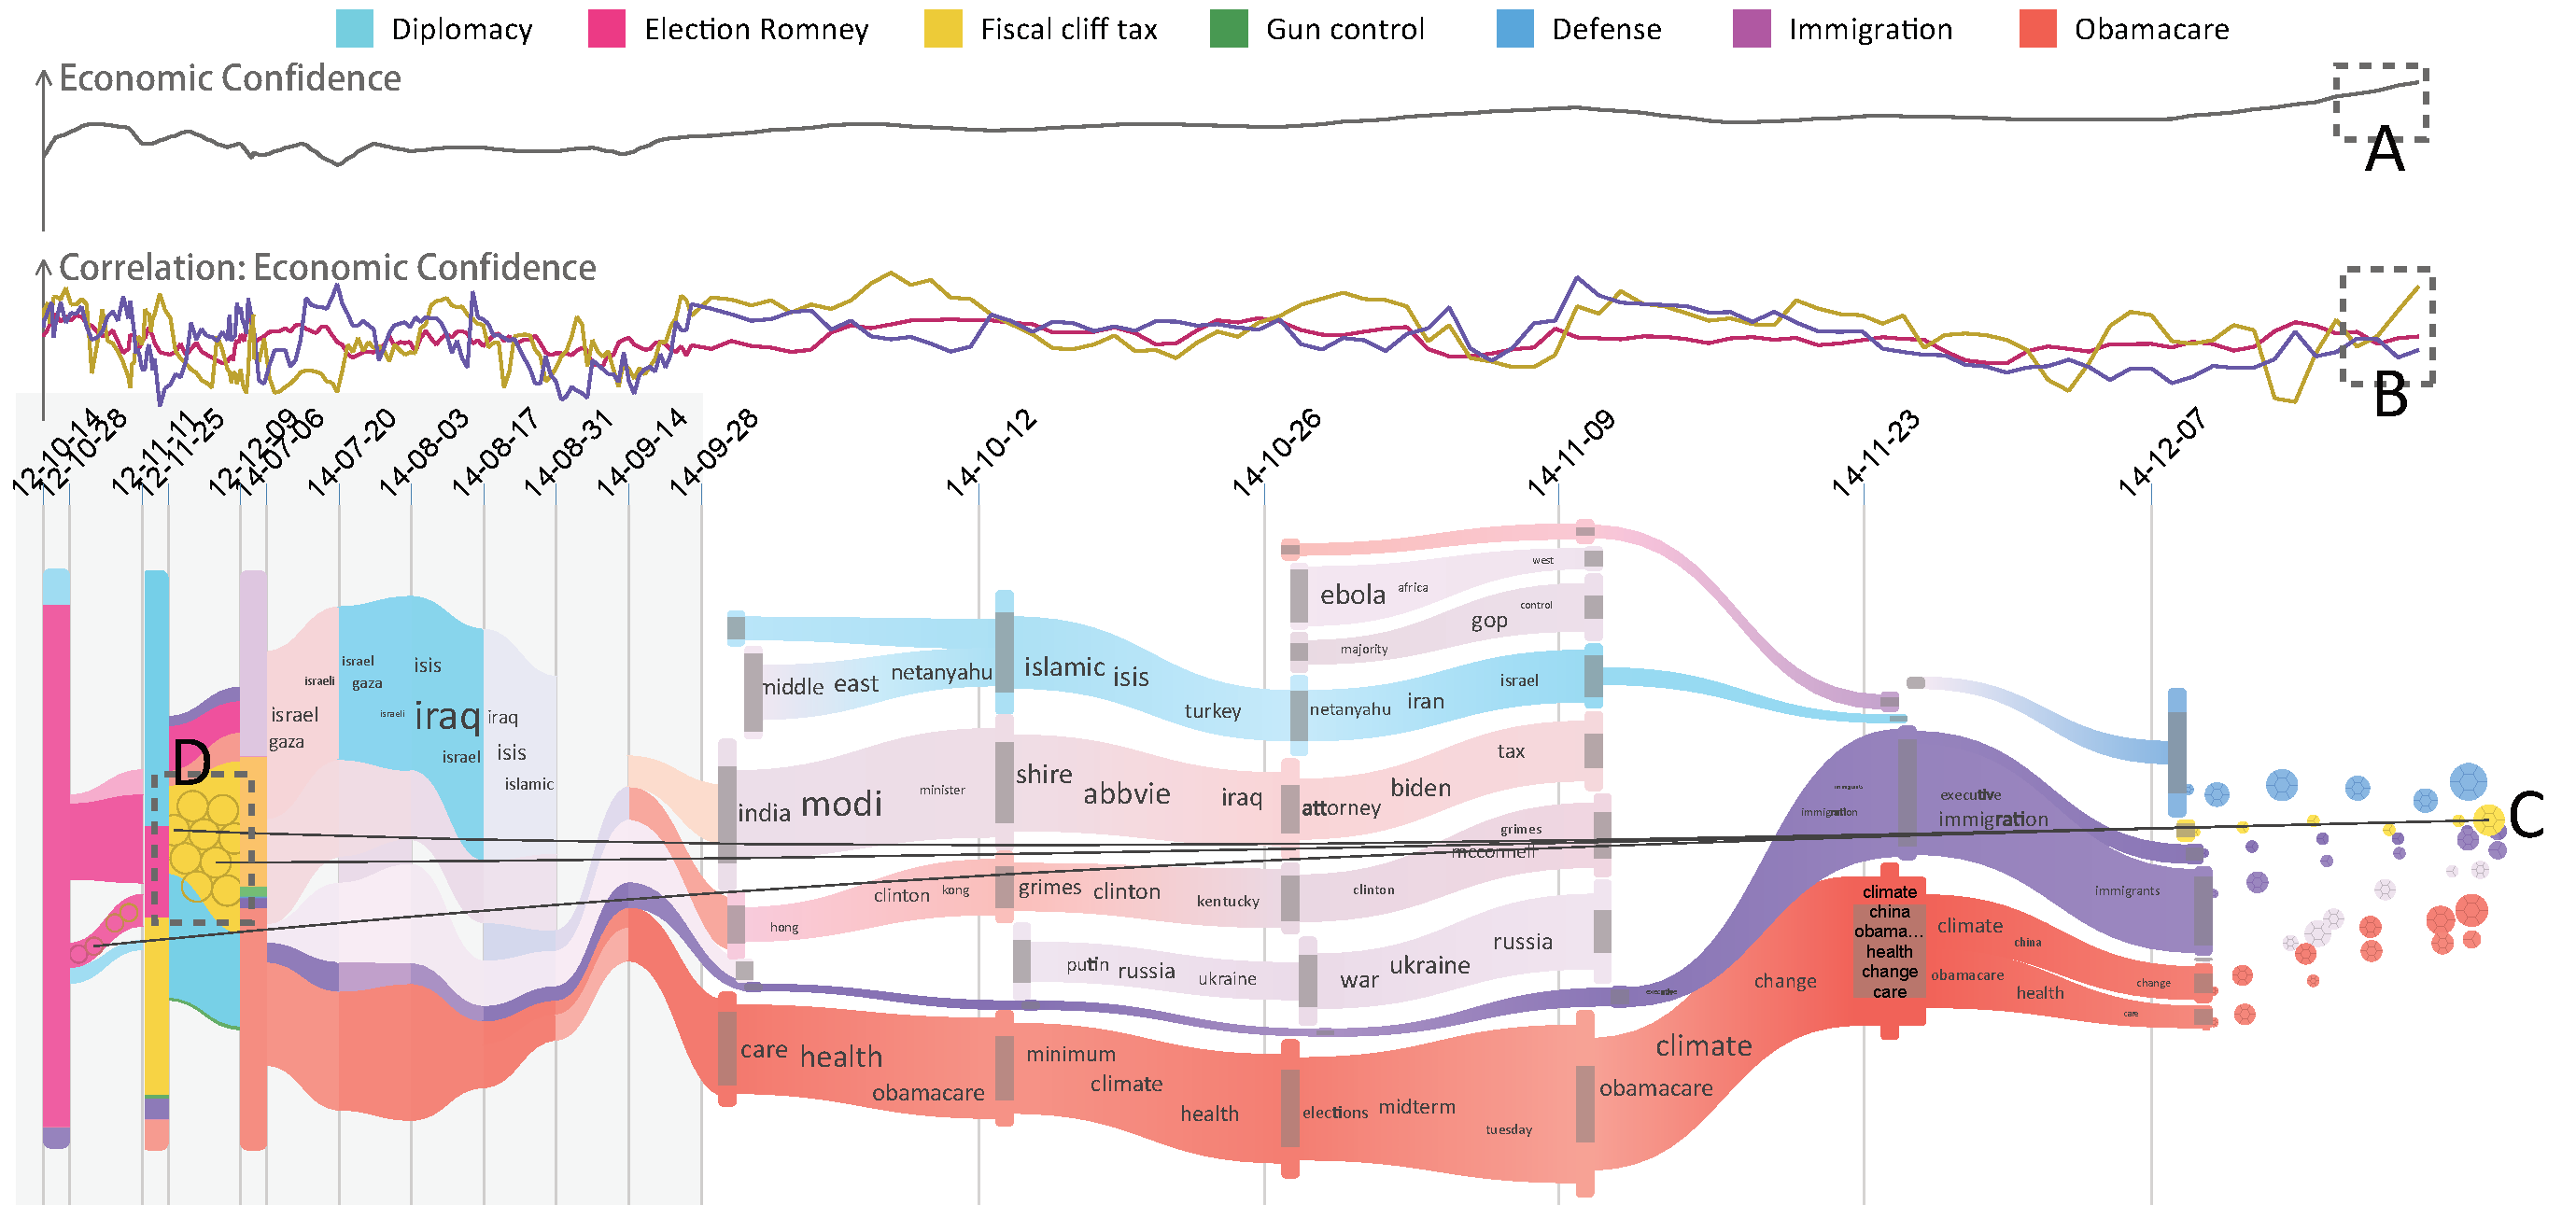
\includegraphics[width=0.85\linewidth]{fig/obamacase2legend}
	\vspace{-2mm}
	\caption{
		%Carry-over effect of the media agenda: the documents about tax raising in 2012 are connected to tax breaks in 2014.
		%Carry-over effect of media agenda: the documents \kg{on} tax \kg{increase} in 2012 are connected to tax breaks in 2014.
		Carry-over effect of media agenda: the documents \kg{on} \docpr{the} tax \kg{increase} in 2012 are connected to tax breaks in 2014.\looseness=-1
	}
	%\vspace{-6mm}
	\label{fig:obamacase2}
	\vspace{-5mm}
\end{figure*}


%After this tragedy people were eager to see tighter gun control (``Gun control petition attracts record interest in US'').
%Obama's action was also in line with public opinion (``Obama's call for action against gun violence''). To see the response of the public to Obama's action professor P1 split the topic and see two major subtopics (Fig.~\ref{fig:obamacase1}G). One subtopic is about Obama's response to the shooting accident (``'')
%This may be one of the leading factors of this increase of the job approval.


%\noindent \textbf{Public attention transited to topic ``Fiscal Cliff.''}
%\noindent \textbf{P ublic attention transited to topic ``\kg{fiscal cliff and taxes}.''}
\noindent \textbf{\normalsize Public attention \dc{transition} to topic ``\kg{fiscal cliff and taxes}.''}
%\textbf{Public approval and public attention transition:}
%Professor (P1) observed an immediate decrease of the precedential approval on Dec. 29, 2012 (Fig.~\ref{fig:obamacase1}D).
%\kg{P1} observed an immediate decrease of the \kg{presidential} approval on Dec. 29, 2012 (Fig.~\ref{fig:obamacase1}D).
%\kg{P1} observed an immediate decrease \dc{in} \kg{presidential} approval on Dec. 31, 2012 (Fig.~\ref{fig:obamacase1}D).
\kg{P1} observed an immediate decrease \dc{in} \docpr{the \kg{presidential} approval rating} on Dec. 31, 2012 (Fig.~\ref{fig:obamacase1}D).
%He was curious about what caused this change.
%The correlation between the precedential approval and topic ``gun control'' decreased to a smaller value (0.12), while its correlation with topic ``fiscal cliff and tax'' increased to the highest (0.51, Fig.~\ref{fig:obamacase1}E).
%The correlation between the \kg{presidential} approval and topic ``gun control'' decreased to a smaller value (0.12), \kg{whereas} its correlation with \kg{the} topic ``fiscal cliff and taxes'' increased to the highest (0.51, Fig.~\ref{fig:obamacase1}E).
The correlation between \dc{presidential} approval and \docpr{the} topic ``gun control'' decreased to a smaller value (0.12), \kg{whereas} its correlation with topic ``fiscal cliff and taxes'' increased to \dc{its} highest (0.51, Fig.~\ref{fig:obamacase1}E).
%After getting a closer look at the ``Fiscal Cliff'' topic,
%He observed that there is a boost of this topic at this time (Fig.~\ref{fig:obamacase1}F).
%Professor P1 commented that this change may be caused by the transition of the public attention to topic ``fiscal cliff and tax.''
%P1 commented that this change \kg{might have been} caused by the transition of the public attention to topic ``fiscal cliff and taxes.''
%P1 \dc{surmised} that this change \kg{might have been} caused by the transition \dc{in} public attention to topic ``fiscal cliff and taxes.''
%This made him more believe that it was the reason.
%He further explained that this topic was talking about the fiscal cliff crisis at the end of 2012.
\kg{P1} explained that this topic was \kg{about} the fiscal cliff crisis at the end of 2012.
%The government was faced with an act taking effect on Jan. 1, 2013.
The government \kg{faced} an act \kg{that would take} effect on Jan. 1, 2013.
%A large tax raising and spending cuts were included in this act.
\kg{Large} tax \kg{increases} and spending cuts were included in this act.
%To postpone this act, the president and the two parties went through a long debate and came to a temporary solution on Jan. 1, 2013.
%To postpone this act, the president and the two \kg{political} parties \kg{debated long and settled with a} temporary solution on Jan. 1, 2013.
To postpone this act, the president and the two \kg{political} parties debated \dc{for a long time} and settled \dc{on} a temporary solution on Jan. 1.
They agreed to postpone the spending cuts until Mar. 1.
%However he did not know what flaws Obama made in handling the crisis which resulted in the critics to him as a president.
%After reading the news he found that people criticized that Obama did not actually want to end this crisis (``Barack Obama and Harry Reid continue their melodramatic playacting, pretending they actually want to stop our nation from going over Obama's Fiscal Cliff'').
%After reading the news\kg{, P1} found that \kg{the public} criticized Obama \kg{for} not actually want to end \kg{the said} crisis (``Barack Obama and Harry Reid continue their melodramatic playacting, pretending they actually want to stop our nation from going over Obama's Fiscal Cliff'').
After reading the news\kg{, P1} found that people \dc{surmised that the president did not truly want the crisis to end}.
 %(``Obama and Reid Continue Playacting'').
%As this topic was about economy, professor P1 switched to the economic confidence index.
%As this topic was \kg{on the} economy, P1 \dc{considered} the economic confidence index.
%As this topic \dc{concerned} economy, P1 \dc{considered} the economic confidence index.
As this topic \dc{concerned} \docpr{the} economy, P1 \dc{considered} the economic confidence index.
%Unsurprisingly, he found a local minimum on Dec. 31, 2012 \kg{(Fig.~\ref{fig:obamacase1}F)}.
Unsurprisingly, a local minimum on Dec. 31, 2012 \kg{(Fig.~\ref{fig:obamacase1}F)} \kg{was found}.
%Because the correlation between this topic and the economic confidence was the highest \kg{(Fig.~\ref{fig:obamacase1}G)},
%The low confidence was possibly caused by raising tax.
%The low confidence \kg{level} was possibly caused by raising tax \kg{rates} \kg{because} the correlation between this topic and the economic confidence was the highest \kg{(Fig.~\ref{fig:obamacase1}G)}.\looseness=-1
The low confidence \kg{level} was possibly caused by raising tax \kg{rates} \kg{because} the correlation between this topic and the economic confidence was \docpr{at its} highest \kg{(Fig.~\ref{fig:obamacase1}G)}.\looseness=-1

%This is consistent with the expert's domain knowledge.

%As the spending cuts of the act was was postponed to Mar. 1, 2013, the professor decided to continue tracking this event.
%As the spending cuts of the act was postponed to Mar. 1, 2013, \kg{P1} decided to continue tracking this event.
As the spending cuts \dc{were} postponed to Mar. 1, \kg{P1} decided to continue tracking this event.
%In the news he learned that this act would have a huge effect on the economy (``Obama said the automatic cuts, known as the sequester, would do great damage to the economy'').
%\kg{Through} the news\kg{,} \kg{P1} learned that this act would have a \kg{significant} effect on the economy (``Bernanke: sequester cuts slow economic recovery'')
He learned that this act would have a \kg{significant} effect on the economy (``Bernanke: sequester cuts slow economic recovery'').
%He found that after two months of negotiation, the two parties did not reach an agreement.
%\kg{and} after two months of negotiation, the two parties \kg{had reached no} agreement.
The spending cuts took effect on Mar. 1.
%On Mar. 1, 2013, he observed another local minimum of the economic confidence \kg{(Fig.~\ref{fig:obamacase1}I)}.
%On \kg{this date}, \kg{P1} observed another local minimum of the economic confidence \kg{(Fig.~\ref{fig:obamacase1}I)}.
On \kg{this date}, \kg{P1} observed another local minimum \dc{in} the economic confidence \kg{(Fig.~\ref{fig:obamacase1}I)}.
%The correlation between the economic confidence and topic ``fiscal cliff and taxes" was the highest \kg{(Fig.~\ref{fig:obamacase1}J)},
%The correlation between the economic confidence and topic ``fiscal cliff and taxes" was \dc{at its} highest \kg{(Fig.~\ref{fig:obamacase1}J)},
The correlation between the economic confidence and \docpr{the} topic ``fiscal cliff and taxes" was \dc{at its} highest \kg{(Fig.~\ref{fig:obamacase1}J)},
%which is in line with the expert's expectation.
which \kg{was} in \kg{accordance} with P1's expectation.
%which was not out of the expert's expectation.
%Professor P1 commented that the streaming visualization is visually appealing and friendly.
%He can use it to examine real-time documents.
%In addition, he can easily tracking the progress of an event and perform analysis to gain insight.
He commented that the streaming visualization \kg{was} visually appealing and practically useful  %shixia to examine
\kg{for examining} real-time documents.\looseness=-1
%\kg{because} tracking the progress of an event and \kg{performing} analysis to gain insight \kg{were easy}.
%\kg{because} tracking the progress of an event and \kg{performing} analysis to gain \dc{insights} \kg{were easy}.

\noindent \textbf{\normalsize Carry-over effect of topic ``fiscal cliff and taxes.''}
%\textbf{Public approval and carry over effect:}
%The case above drew great interest of professor P1.
%professor P1 wanted to follow the subsequent development of this topic.
P1 wanted to follow the subsequent development of this topic.
%He found that topic ``fiscal cliff and tax" (yellow) appeared again on Dec. 21, 2014 (Fig.~\ref{fig:obamacase2}).
%He found that topic ``fiscal cliff and tax" (yellow) appeared again on Dec. 7, 2014 (Fig.~\ref{fig:obamacase2}).
%He found that topic ``fiscal cliff and taxes" (yellow) appeared again on Dec. 7, 2014 (Fig.~\ref{fig:obamacase2}).
%He found that topic ``fiscal cliff and taxes" (yellow) appeared again on Dec. 7, 2014 (Fig.~\ref{fig:obamacase2}).
He found that \docpr{the} topic ``fiscal cliff and taxes" (yellow) appeared again on Dec. 7, 2014 (Fig.~\ref{fig:obamacase2}).
%This topic talked about tax breaks at the end of 2014. %for retailers and teachers
%This topic \kg{focused on} tax breaks at the end of 2014. %for retailers and teachers
This topic \dc{concerned} tax breaks at the end of 2014. %for retailers and teachers
%At this time, the economic confidence index had a remarkable increase (Fig.~\ref{fig:obamacase2}A).
%At this time, the economic confidence index \kg{showed} a remarkable increase (Fig.~\ref{fig:obamacase2}A).
At this time, the economic confidence index \dc{experienced} a remarkable increase (Fig.~\ref{fig:obamacase2}A).
%Because the correlation between this index and topic ``fiscal cliff and tax" was the highest (0.44, Fig.~\ref{fig:obamacase2}B), P1 speculated that intensive discussions on tax breaks in this topic is a potential reason.
%Because the correlation between this index and topic ``fiscal cliff and taxes" was the highest (0.44, Fig.~\ref{fig:obamacase2}B), P1 speculated that \dc{intense} discussions on tax breaks \dc{concerning} this topic \dc{were} a potential reason.
Because the correlation between this index and \docpr{the} topic ``fiscal cliff and taxes" was \docpr{at its} highest (0.44, Fig.~\ref{fig:obamacase2}B), P1 speculated that \dc{intense} discussions on tax breaks \dc{concerning} this topic \dc{were} a potential reason.
%P1 speculated that \kg{the} topic \kg{on tax breaks} \kg{was} a potential reason \kg{for the high} correlation \kg{of the} topic ``fiscal cliff and taxes" (0.44, Fig.~\ref{fig:obamacase2}B).
%P1 was curious why such a small topic had a significant influence on the economic confidence.
\kg{P1} was curious \kg{about the} significant influence \kg{of this small topic} on economic confidence.
%To this end, he linked the largest document cluster (Fig.~\ref{fig:obamacase2}C) at this time to the previous relevant documents.
To this end, \kg{P1} linked the largest document cluster (Fig.~\ref{fig:obamacase2}C) at this time to the previous relevant documents.
%There are several documents appeared during the period of fiscal cliff crisis in 2012 (Fig.~\ref{fig:obamacase2}D).
\kg{Several} documents appeared during the period of \kg{the} fiscal cliff crisis in 2012 (Fig.~\ref{fig:obamacase2}D).
%At that time, the government wanted to raise tax due to fiscal cliff and this topic was the dominant topic in media (the yellow topic in Fig.~\ref{fig:obamacase2}(a) and (b)).
At that time, the government wanted to raise \kg{taxes because of the} fiscal cliff and this topic was dominant in \kg{the} media (yellow topic in Figs.~\ref{fig:obamacase1}(a) and (b)).
%It caused a decrease of the economic confidence.
%Professor P1 commented that this can be regarded as the carry-over effect \cite{carry-over} in his field.
%\kg{P1} commented that this \kg{fact} \kg{could} be regarded as the carry-over effect \cite{carry-over} in \kg{the field of media and communication}.
\kg{P1} commented that this \kg{fact} \kg{could} be regarded as \dc{a} carry-over effect \cite{carry-over} in the field of media and \dc{communication}.
%He further explained, ``The fiscal cliff crisis left a profound impression on the public and had a great influence to the economic confidence at that time.
\kg{P1} further explained, ``The fiscal cliff crisis left a profound impression on the public and had a great influence \kg{on} the economic confidence at that time.
As a result, this influence can be carried over to the relevant topic later even if it is a smaller one.''

%However he was suspicious that this effect could be carried over to two years later.
%To make his analysis complete,

%To verify his assumption that topic ``fiscal cliff and tax" was the major reason, the professor wanted to .
%To find or exclude other possible reasons, the professor continued to check other topics (``defense'' and ``immigration'') occurred during that time.
%To find or exclude other possible reasons, \kg{P1 checked} other topics (``defense'' and ``immigration'') \kg{during that period.}
%%The correlation between the economic confidence and these topics are low (``defense:'' 0.10; ``immigration:'' -0.07).
%%The correlation between the economic confidence and these topics \kg{were} low (``defense:'' 0.10; ``immigration:'' -0.07).
%The correlation between the economic confidence and these topics \dc{was} low (``defense:'' 0.10; ``immigration:'' -0.07).
%%He then excluded these two topics from possible reasons.
%%\kg{P1} then excluded these two topics from \kg{being} possible reasons.
%He then excluded these two topics from being possible reasons.
%%In the visualization, he found another large topic that he did not pay attention to before, ``Obamacare'' (purple).
%In the visualization, \kg{P1} found another large topic \kg{that was previously missed,} ``Obamacare'' (red).
%He added this topic to the focus list and regenerated the visualization.
%%\kg{This} topic \kg{was added} to the focus list and regenerated the visualization.
%%He checked the correlation between topic ``Obamacare'' and the economic confidence and found the correlation is low (0.20).
%\kg{The} correlation between ``Obamacare'' and economic confidence \kg{was} low (0.20).
%%Thus he also excluded this topic.
%Thus\kg{,} this topic \kg{was also excluded.}
%%Finally, the expert concluded that tax breaks may be the leading cause of the economic confidence increase.
%%Finally, the expert concluded that tax breaks \kg{might} be the leading cause of the economic confidence increase.
%\kg{This led to the conclusion that tax breaks were potentially the leading cause for the increase in economic confidence.\looseness=-1}
%Professor P1 was very surprised that the carry-over effect could be such strong that even after two years the topic could still have such a strong influence on the economic confidence.

%444,432 news articles that contain the keyword ``Obama,'' were collected from Sep. 1, 2012 to Jan. 14, 2013.
%Grouped by week, the articles were organized into 18 topic trees. %(Fig.~\ref{fig:obamatree}).
%%The average number of the first level nodes is 41, and the tree depth is 5($\pm 1$).
%The tree depths varied from 4 to 5, the total node numbers changed from 144 to 297, and the node
%number of the first level ranged from 18 to 79.
%
%To provide an overview of the news data to users, our system automatically extracted several initial focus nodes that can suitably represent the dataset and are distinct from one another.
%In our implementation, a clustering method, the mean-shift algorithm, was utilized to cluster the topic at the first level because it is the most abstract level and can represent the topic tree very well.
%Four clusters were detected in the Obama data.
%For each cluster, we selected the node closest to the cluster center as a focus node.
%Four focus nodes were automatically derived to generate the default overview (Fig.~\ref{fig:obama}(a)).
%In the overview, the four colors represent four different topics: ``Iran'' (red), ``Tax'' (yellow), ``Debate'' (green), and ``Gun Control'' (purple).
%As shown in Fig.~\ref{fig:obama}(a), significant variations existed; however, some overall patterns clearly stood out.
%The green and yellow topics were dominant and divided the entire time period into two parts.
%The red topic was small but persistent and the purple one was large but irruptive.
%
%In the first half of the time period (before Nov. 3), the ``Debate'' (green) topic dominated and unsurprisingly ended in the week of Nov. 6, 2012, the date when Obama was reelected as president.
%In addition, the ``Tax'' (yellow) topic was partially related to the ``Debate'' (green) topic from time to time.
%Initially, the yellowish green topic (marked as \textbf{A} in Fig.~\ref{fig:obama}(a)), a mixed topic of ``Debate'' and ``Tax,'' merged with the green one.
%This merging was caused by the tax-related debates (``Obama, Romney Clash on Economy, Taxes in First Debate'').
%The yellowish green topic gradually split from the green one because its focus shifted to the economy, jobs, and the fiscal cliff.
%If users are interested in tracking the mixed topic, they could interactively split the topic nodes and extract them from the green topic (Fig.~\ref{fig:obama}(b)).
%
%
%Similarly, the ``Iran'' (red) topic  interacted with the ``Debate'' (green) topic in the week of Oct. 20 (marked as \textbf{B} in Fig.~\ref{fig:obama}(a)).
%After splitting the topic nodes into small ones (Fig.~\ref{fig:obama}(c)), a red topic node that contained several news articles on ``Iran'' was observed
%For example, one of them is ``Obama, Romney on Israel and Iran.'' This article clearly indicates why these two topics merged.
%
%After the week of Nov. 3 (the second half of the time period), the ``Tax'' (yellow) topic dominated the view.
%Considering that it has fewer connections with other topics, it was more isolated than the ``Debate'' topic.
%Within these topics, the yellow nodes were almost fully connected with one another; thus, the ``Tax'' was also a relatively stable topic.
%
%Although the ``Tax'' (yellow) topic was dominant during this time period, two greenish nodes (marked as \textbf{C} and \textbf{D} in Fig.~\ref{fig:obama}(a)) still appeared.
%Clearly, these two topics have different evolution patterns.
%Judging from the connections between \textbf{C} and the other nodes, \textbf{C} was likely a momentary topic.
%To verify this hypothesis, we examined \textbf{C}'s content and found that it was focused on ``Romney blames loss on Obama's `gifts' to voters,'' which was indeed a momentary event.
%On the other hand, \textbf{D} was fully connected to the yellow nodes. This connection indicates \textbf{D} contains news articles related to both the ``Debate'' and ``Tax'' topics. For example, one of the articles had the title ``GOP fights President Barack Obama on his campaign promise to raise taxes on the rich.''\looseness=-1
%
%
%The ``Gun Control'' (purple) topic, which was caused by the Connecticut Elementary School massacre on Dec. 14, 2012, was then explored.
%The event caused a topic burst in the week of Dec. 15.
%Its horizontal offset indicates that it is a high-level topic node.
%%Although the topic has a burst in the week of December 15, our system still finds several related topics, colored in purple, before the burst (marked as dotted rectangles in Fig.~\ref{fig:obama}(a)).
%%Since they are highly related to our focus node, they are still successfully separated from the others.
%%For example, in the week of Dec. 1, 2012 (marked as \textbf{E}), a node of only five documents talks about ``Obama to Push Gun Control in Second Term?''.
%Then we split the big purple node and checked the two smaller topics in it (Fig.~\ref{fig:obama}(d)).
%The lower node was mainly about the public discussion on gun control.
%The strong connection of this node to the topic on the right indicates that it was still the major topic at the next time point.
%When the node was split further, more detailed topics revealed themselves (Fig.~\ref{fig:obama}(e)).
%From top to bottom, these topics were ``NRA calls for armed guards at every school,'' ``Obama turns to Biden on gun control measures,'' ``Guns fly off shelves,'' ``Assault weapons ban,'' and ``Connecticut school shooting: how to talk to your kids'' (marked as \textbf{F} to \textbf{J}, respectively).
%The upper node, which represents follow-up news to the tragedy, has weaker connections to the right.
%This condition indicates that the topic shrunk considerably at the next time point.

%  \vspace{-4mm}

%\begin{figure}[t]
%  \centering
%  \includegraphics[width=\columnwidth]{fig/2clintonoverview}
%    \vspace{-4mm}
%  \caption{
%%  \small
%  Topics related to ``Bill Clinton'' and ``Hillary Clinton.''\looseness=-1}
%  \vspace{-3mm}
%  \label{fig:2clintonoverview}
%\end{figure}



%from Shixia, the below story can be deleted if the qualitative evaluation need more space.



%The search function can help users explore more specific topics.
%For example, we entered ``Clinton'' in the search box.
%The first topic node recommended by our system is about the speech at the Democratic National Convention on Sep. 5, 2012.
%We selected it as the focus node and visualized the result.
%As shown in Fig.~\ref{fig:clintonoverview}, the topic was only active in the first week (marked as \textbf{A}).
%However, in the week of Oct. 20, a small but highly related topic node appeared (marked as \textbf{B}).
%We clicked it to see the detailed content and found that it contained two sub-topic nodes: ``Bill Clinton to rally for Obama at Springs Preserve'' and ``Hillary Clinton says she's `unlikely' to stay Secretary of State'' (marked as \textbf{C}).
%To further explore these nodes, we regarded both nodes as new focus nodes and transformed the visualization.
%Fig.~\ref{fig:2clintonoverview} shows that the two Clintons mainly have one overlapping topic (marked as \textbf{D}), which is ``Bill Clinton's DNC speech: Setting the stage for Hillary in 2016?''
%
%%In the middle of Fig.~\ref{fig:2clintonoverview}, our tree cut algorithm successfully splits the context topic and reveals two small relevant topics hidden inside, which are a discussion about ``Poll: Clinton favored in 2016 in Iowa''.
%
%The topics on Hillary Clinton in the top of Fig.~\ref{fig:2clintonoverview} can be  divided into two parts (marked by \textbf{F} and \textbf{G}).
%\textbf{F} is about the Libya Attack, in which Hillary Clinton was highly involved.
%In the week of Oct. 13, the article with the title ``Hillary Clinton Takes Blame for Benghazi Attack'' ended that topic (marked by \textbf{E}).
%\textbf{G} contains two separate topics related to Hillary Clinton whose colors indicate that one is more relevant to the focus than the other.
%In fact, the greener one is about Hillary Clinton herself.
%For example, two articles have the titles ``Clinton is the people's choice for 2016 Prez bid: Poll,'' and ``Obama calls Clinton to wish her well as she recovers from concussion.''
%However, the other is about the secretary of state candidates, in which Hillary Clinton is partially involved.




%% !TEX root = EvoTree-KDD.tex

\section{Potential Applications}\label{sec:application}

We deployed the system as an internal desktop application within Microsoft. A panel of experts, including customer relationship managers, public relations managers, and researchers, systematically evaluated and investigated the potential applications of the system.  Several highly promising applications were identified.

%We invited several experts, including 3 customer relationship managers, 3 public relations managers, and 4 researchers, to systematically evaluate and discuss the potential usage of the system.


First, our system can be employed in customer relationship management to help analysts fully understand customer-related information on social media.
A variety of social media outlets enable customers to communicate with each other more easily and take a more active role as market players~\cite{Hennig2010}.
%Since the buzz of the crowd on social media provides a great deal of information that
%was not available before, businesses have started leveraging social media to profile customers, derive brand perception, understand buying trends, and improve customer satisfaction.
The implication for businesses is obvious: they need to understand what customers are saying about them in various social media outlets.
For this reason, customer relationship managers are very interested in using the system to quickly understand customers' comments and feedbacks on social media.
For example, a customer relationship manager utilized the system to analyze customer feedback related to ``Xbox'' on Twitter and blogs.
He appreciated the topic hierarchies provided by the system, which enabled him to immediately identify overall patterns as well as directly interact with the visualization to examine the finer-grained topics.
He commented, ``This is very helpful in finding something unexpected.''

Second, public relations managers claimed that the system can help them better analyze company-related information, such as news, blogs, and microblogs.
For example, a Microsoft public relations analyst wants to analyze a number of important events related to the company that occurred in the first half of 2013.
These events are the announcement of the new Xbox, Motorola suing the company, and the release of Windows 8.
To analyze these events, the public relations analyst employed the system to examine the Microsoft-related news stream and understand the major topics and how they have changed over time.
With the system, the analyst could better understand how these events are related to one another at different granularities and their impact over time.
Furthermore, he can determine whether the company's public relations strategies have succeeded (e.g., the amount of the excitement generated by the product release).

Finally, researchers utilized our system to study major research topics in their fields as well as the splitting/merging relationships among the topics of interest over time.
With this toolkit, they easily identified the research topics and related publications that match their research interest.
Interestingly, a sociology PhD student found that he could use the system to study the media framing effects in a news corpus.
He was intrigued when he found that a sub-topic changed its parent between two adjacent trees.
In his exploration, the sub-topic exemplified by the keywords ``Windows, Kinect" changed its parent from ``Windows" to ``Xbox."
He said, ``Parent topics provide the context for the sub-topics.
A concrete sub-topic such as ``Kinect'' can be mentioned in the context of ``Windows'' in the first week, and in the context of ``Xbox'' in the next week.
This defines different perspectives or ways of communicating about topics.
This phenomenon is widely studied in our field and is referred to as \textbf{media framing}.
I believe this system can definitely help detect such framing phenomena." 
% !TEX root = EvoTree-KDD.tex

\section{Discussion and Future Work}\label{sec:conclustion}
In this paper, we have presented a novel visual analytics system to help users explore and understand hierarchical topic evolution in high-volume text streams.
%\kg{This paper reports on} a novel visual analytics system to help users explore and understand hierarchical topic evolution in a text stream, at different \kg{abstraction} levels.
Powered by the streaming tree cut model and the corresponding visualization, the system allows users to analyze hierarchical topics at different \dc{granularities,} as well as their evolution patterns over time.
%Powered by the evolutionary tree cut model and the corresponding visualization, \kg{this} system allows users to analyze hierarchical topics at different granularities \kg{and} their evolution patterns over time.
%In addition, it allows users to interactively customize and refine the visualization based on their interests.
%In addition, it \kg{enables} users to customize interactively and refine visualization based on their interests.
In addition, it \kg{enables} users to interactively customize and refine \dc{the} visualization based on their interests.
%A quantitative evaluation and a case study were conducted to demonstrate the effectiveness and usefulness in text stream analysis.
%A quantitative evaluation and a case study were conducted to demonstrate the effectiveness and usefulness \kg{of the system} in text stream analysis.
A quantitative evaluation and two case studies were conducted to demonstrate the effectiveness and usefulness \kg{of the system} \dc{for} text stream analysis.

Although the system performs well when analyzing the evolution of hierarchical topics, it can still be improved.
%First, one component of our system is the evolutionary tree clustering algorithm. This algorithm is effective in constructing a sequence of topic trees with high fitness and smoothness.
First, one component of our system, the evolutionary tree clustering algorithm, is effective in constructing a sequence of topic trees with high fitness and smoothness.
%However, solely relying on the optimization results is not always effective because the tree cut algorithm may be imperfect and different users may have different needs.
However, relying \kg{solely} on the optimization results is not always effective because the tree clustering algorithm may be imperfect and different users may have different \kg{requirements}.
%To solve this problem, it would be desirable to study how to leverage a user's domain knowledge in our system and allow him/her to better express and define the information needs.
Studying how to leverage the domain knowledge of a user in our system and allow him/her \kg{to express and define information requirements can help solve the aforementioned problem.}
%This topic is interesting to pursue in the future.
\kg{This noteworthy topic can be pursued} in the future.
%Second, we only utilize the horizontal offset to encode the tree depth but ignore the tree general structures.
%Second, we only utilize the horizontal offset to encode tree depth but ignore the general structures \kg{of a tree}.
Second, we only \docpr{utilized} the horizontal offset to encode tree depth but \docpr{ignored} the general \docpr{structure} \kg{of a tree}.
%However, in some cases, users may want to examine each tree structure and obtain a complete overview of evolving topic trees.
However, users may want to examine each tree structure and obtain a complete overview of evolving topic trees \kg{in several cases}.
%In the future, we also plan to enable the ability of tree exploration in the next version of the system and allow users to explicitly explore the topic hierarchical structures.
%\kg{We} also plan to enable tree exploration \kg{capability} in the next version of the system and allow users to explore topic hierarchical structures \kg{explicitly}.
\kg{We} also plan to enable tree \docpr{exploration in} the next version of the system and allow users to \docpr{explicitly} explore topic hierarchical \docpr{structures.}


%\pei{We can shorten the reference list using abbreviations (i.e., ``first author et al.'') and omitting page numbers.  This will give us more space so that the figures are not squeezed.  Some reviewers may complain if we use vspace too much in the main body of the paper.}

%our visualization highly depends on the back-end evolutionary tree structures.
%Wrong structures cannot make reasonable visualizations.
%However, the generation process is highly complicated and sensitive to parameters.
%Since users cannot participate in the tree generation process, it is hard to produce desirable structures based on user domain knowledge.
%Therefore, adding user controls to the process is one important future work for our system.
%Allowing users to refine the structures based on their domain knowledge can greatly improve the resulting tree sequence, thus enhance the visual exploration experience.
%Second, tree structures are only partially encoded in our system.

\section{Acknowledgements}
This research was supported by National Key Technologies R\&D Program of China (No. 2015BAF23B03), the National Natural Science Foundation of China (No.s 61373070, 61272225, 61572274), and a Microsoft Research Fund (No. FY15-RES-OPP-112). 
}

%% if specified like this the section will be ommitted in review mode
%\acknowledgments{
% The authors would like to thank Yuzuru Tanahashi for providing the comparison data and helping generate some of the comparison examples and Stephen Lin for proofreading the paper.\looseness=-1}
%%\newpage
%\clearpage
\small
\bibliographystyle{abbrv}
%\addtolength{\itemsep}{5ex}
\bibliography{reference}

  % sigproc.bib is the name of the Bibliography in this case

%1 page

\vspace{-10mm}
\begin{IEEEbiography}[{\includegraphics[width=1in,height=1.25in,clip,keepaspectratio]{fig/shixia.jpg}}]{Shixia Liu}
is an associate professor at Tsinghua University. Her research interests include visual text analytics, visual social analytics, and text mining. She worked as a research staff member at IBM China Research Lab and a lead researcher at Microsoft Research Asia.
She received a B.S. and M.S. from Harbin Institute of Technology, a Ph.D. from Tsinghua University. 
She is an associate editor of IEEE TVCG.
%
\vspace{-8mm}
\end{IEEEbiography}

\vspace{-8mm}
\begin{IEEEbiography}[{\includegraphics[width=1in,height=1.25in]{fig/Jialun.jpg}}]{Jialun Yin} is a PhD candidate in the Department of Computer Science and Technology at Tsinghua University, China.
His research interests include visual text analytics and data mining.
He received a BS degree in Computer Science from Tsinghua University.
\vspace{-8mm}
\end{IEEEbiography}

\vspace{-8mm}
\begin{IEEEbiography}[{\includegraphics[width=1in,height=1.25in]{fig/xiting.jpg}}]{Xiting Wang} is a PhD candidate in the Institute for Advanced Study at Tsinghua University, China.
Her research interests include visual text analytics and text mining.
She received a BS degree in Electronics Engineering from Tsinghua University.
\vspace{-8mm}
\end{IEEEbiography}

\vspace{-8mm}
\begin{IEEEbiography}[{\includegraphics[width=1in,height=1.25in,clip,keepaspectratio]{fig/weiwei.jpg}}]{Weiwei Cui}
is a researcher in the Internet Graphics Group at Microsoft Research Asia.
His research interests include visualization and visual analytics, with emphasis on text and graph data.
He received a PhD in computer science from Hong Kong University of Science and Technology.


%
\vspace{-8mm}
\end{IEEEbiography}

\vspace{-8mm}
\begin{IEEEbiography}[{\includegraphics[width=1in,height=1.25in,clip,keepaspectratio]{fig/kelei.jpg}}]{Kelei Cao}
is an undergraduate in the Department of Computer Science and Technology at Tsinghua University, China. His research interests include visual text analytics.

%
\vspace{-8mm}
\end{IEEEbiography}

\vspace{-8mm}

\begin{IEEEbiography}[{\includegraphics[width=1in,height=1.25in,clip,keepaspectratio]{fig/jian.jpg}}]{Jian Pei}
is currently the Canada Research Chair (Tier 1) in Big Data Science and a professor at the School of Computing Science and the Department of Statistics and Actuarial Science at Simon Fraser University, Canada. He received his Ph.D. degree at the same school in 2002 under Dr. Jiawei Han's supervision.  His research interests are to develop effective and efficient data analysis techniques for novel data intensive applications.  He has published prolifically and is one of the top cited authors in data mining.  He received a series of prestigious awards.  He is also active in providing consulting service to industry and transferring the research outcome in his group to industry and applications.  He is an editor of several esteemed journals in his areas and a passionate organizer of the premier academic conferences defining the frontiers of the areas. He is an IEEE Fellow.
%
%\vspace{-8mm}
\end{IEEEbiography}


\end{document}

